\chapter{TỔNG QUAN: HỆ KHUYẾN NGHỊ, NHỮNG PHƯƠNG PHÁP TIẾP CẬN PHỔ BIẾN VÀ XU HƯỚNG}
\ifpdf
    \graphicspath{{Chapter1/Chapter1Figs/PNG/}{Chapter1/Chapter1Figs/PDF/}{Chapter1/Chapter1Figs/}}
\else
    \graphicspath{{Chapter1/Chapter1Figs/EPS/}{Chapter1/Chapter1Figs/}}
\fi

\section{Giới thiệu}
%Trước đây, con người thường khó ra quyết định vì không có đủ thông tin cần thiết. Ngược lại, ngày nay quá nhiều thông tin có giá trị có thể giúp con người đưa ra những quyết định đúng, phù hợp. Nhưng thật trớ trêu là con người không đủ thời gian và khả năng để sắp xếp, chọn lọc ra những thông tin thật sự có giá trị. Hệ khuyến nghị là giải pháp giúp con người có thể đương đầu với một lượng thông tin khổng lồ đang bùng nổ trên mạng internet, giúp con người có thể đưa ra các quyết định đúng, phù hợp. Hệ khuyến nghị giúp thông tin liên quan tự tìm đến người dùng, thay vì người dùng phải tự đi tìm thông tin như các hệ thống tìm kiếm thông tin truyền thống. "Chúng ta đang ra khỏi thời đại thông tin và bước vào thời đại của khuyến nghị", phát biểu này là khẩu hiệu của hội thảo chuyên đề ACM RecSys-2012, một hội thảo uy tín về hệ khuyến nghị do ACM phối hợp với các cơ quan nghiên cứu tổ chức mỗi năm một lần.\footnote{http://recsys.acm.org/2012/, truy cập lần cuối ngày 5/2/2014}
%
%Theo Gunawardana và Shani \cite{GunawardanaS09}, khó có thể đưa ra một định nghĩa chính xác cho hệ khuyến nghị. Nhiều hệ thống với những mục tiêu và hành vi khác nhau được gom nhóm lại và gọi chung là hệ khuyến nghị. Tùy vào công việc hay phương pháp thực hiện khuyến nghị mà hệ khuyến nghị được phân thành nhiều nhóm khác nhau. Chẳng hạn, Gunawardana và Shani đã phân hệ khuyến nghị thành 3 nhóm chính dựa trên công việc khuyến nghị mà hệ thống cần thực hiện: (1) Tiên đoán đánh giá của người dùng; (2) Khuyến nghị những đối tượng tốt; (3) Tối ưu tính tiện ích của hệ thống khuyến nghị (hình \ref{fig:figure_1_0}). Bênh cạnh đó, các tác giả Adomavicius và Tuzhilin \cite{Adomavicius:2005:TNG:1070611.1070751}, Stefanidis và cộng sự \cite{StefanidisNNK12}, Bobadilla và cộng sự \cite{Bobadilla2013109}, cũng như một số nghiên cứu phổ biến khác thì phân hệ khuyến nghị thành các nhóm chính dựa trên phương pháp tiếp cận: (1) Tiếp cận nội dung; (2) Tiếp cận Lọc cộng tác; (3) Tiếp cận lai: kết hợp tiếp cận nội dung và lọc cộng tác. 

Dựa trên kết quả khảo sát, chương này sẽ phát biểu lại một cách hình thức bài toán khuyến nghị trong trường hợp tổng quát, tập trung trình bày và phân tích ưu điểm, hạn chế của những phương pháp tiếp cận truyền thống cũng như xu hướng mới cho hệ khuyến nghị.

\section{Khái niệm Hệ khuyến nghị}
Hệ khuyến nghị, tiếng anh là Recommender Systems hoặc Recommendation System, là những hệ thống được thiết kế để hướng người dùng đến những đối tượng quan tâm, yêu thích, khi lượng thông tin quá lớn vượt quá khả năng xử lý của người dùng \cite{PaulResnick:1997_RecSystems_ACM, Robin:2002:HybridRS_Survey}. 

Theo Ricci và cộng sự \cite{RicciFrancesco:2011}, hệ khuyến nghị là những công cụ phần mềm, kỹ thuật cung cấp những đề xuất các đối tượng có thể hữu ích với người dùng. Những đề xuất liên quan đến quyết định của người dùng như: sản phẩm nào nên mua, bài hát nào nên nghe, hay tin tức nào nên đọc. Tác giả Gunawardana và Shani thì cho rằng rất khó có thể đưa ra một định nghĩa cho hệ khuyến nghị, bởi vì những hệ thống với nhiều mục tiêu và hành vi khác nhau được gom nhóm lại và đặt tên là hệ khuyến nghị \cite{GunawardanaS09}. Tác giả đã phân loại hệ khuyến nghị thành nhiều nhóm khác nhau dựa trên công việc mà hệ thống thực hiện (hình \ref{fig:figure_1_0}).

\begin{figure}[ht]
\begin{center}
\advance\leftskip-3cm
\advance\rightskip-3cm
  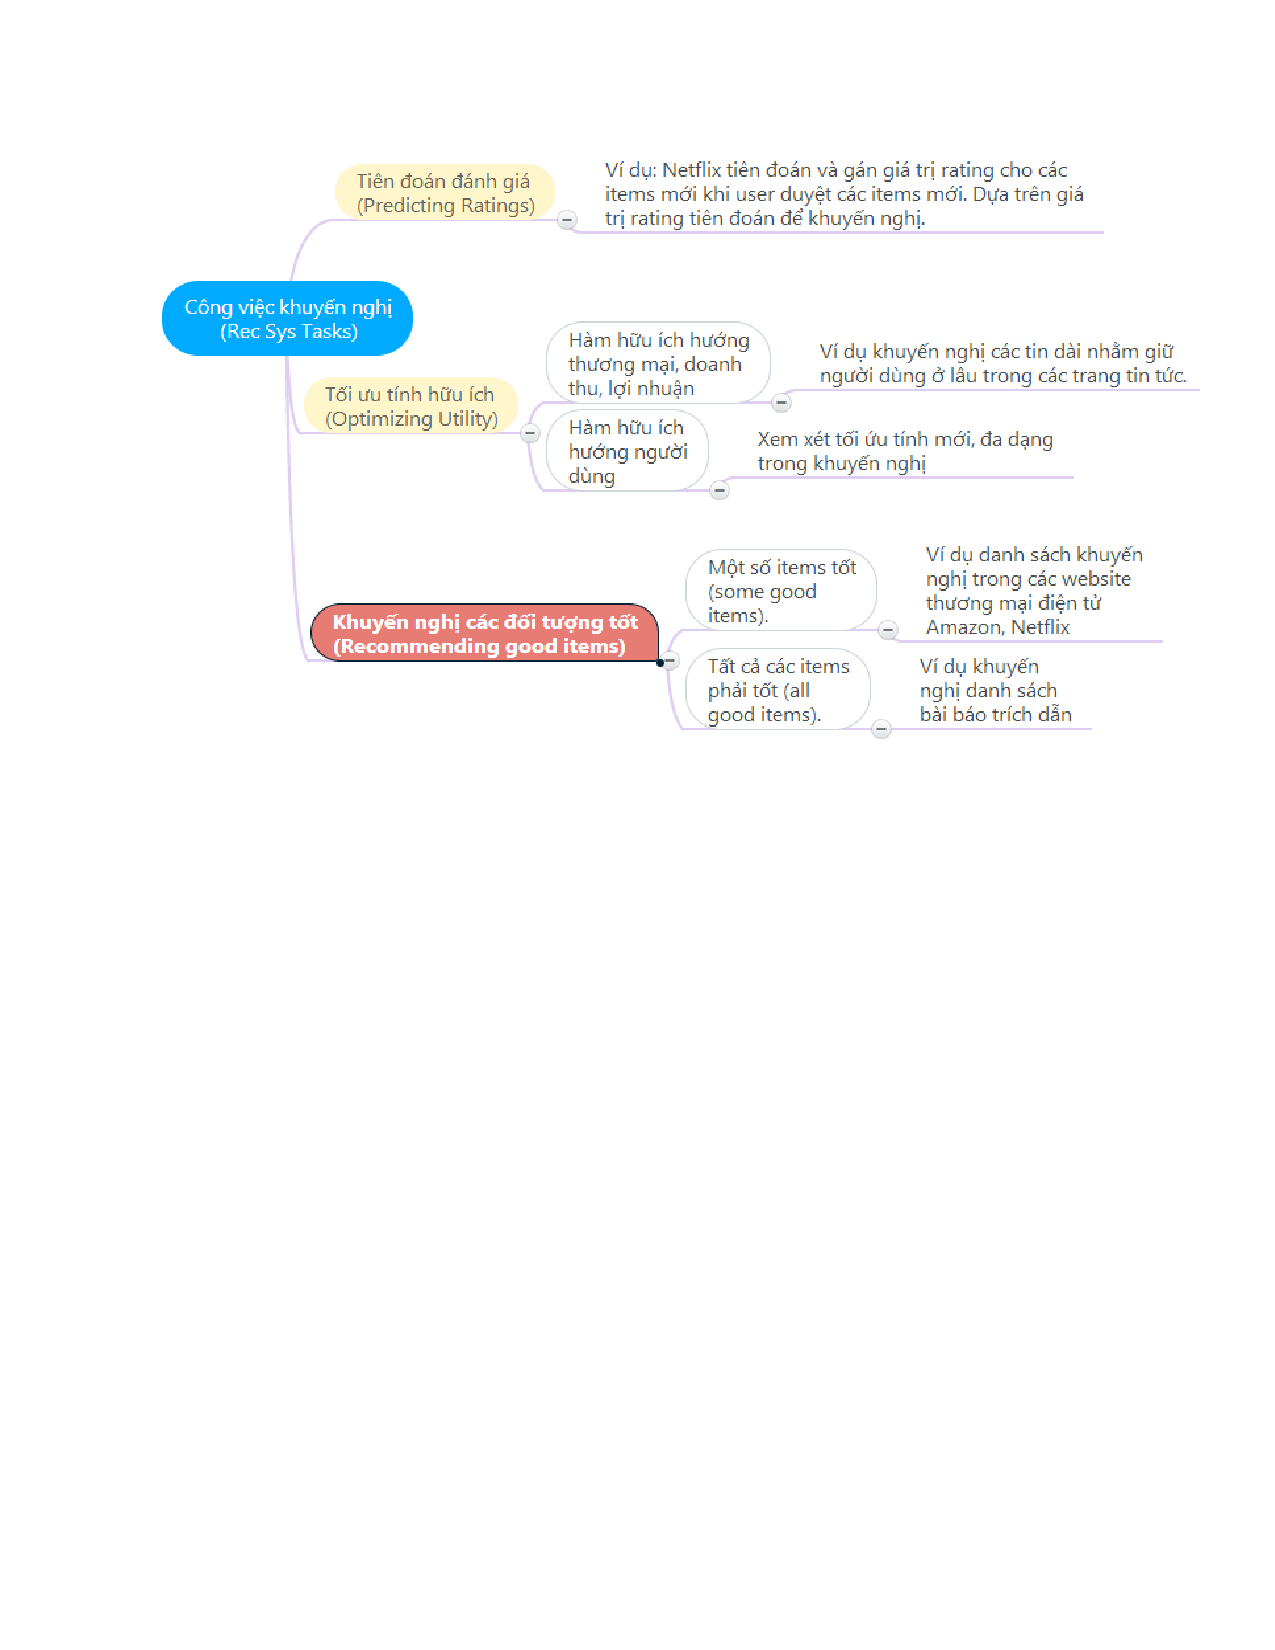
\includegraphics[width=0.85\textwidth]{Figure_1_0.pdf}
  \caption{Phân loại hệ khuyến nghị dựa trên công việc khuyến nghị}\label{fig:figure_1_0}
\end{center}
\end{figure}

Chúng ta có thể hiểu hệ khuyến nghị là những hệ thống, công cụ, kỹ thuật, được thiết kế để hướng người dùng đến những đối tượng quan tâm, yêu thích, khi lượng thông tin quá lớn vượt quá khả năng xử lý của người dùng. Khi tích hợp vào các hệ thống thương mại điện tử cũng như các hệ thống tìm kiếm, hệ khuyến nghị sẽ giúp người dùng dễ dàng hơn trong quá trình tìm kiếm thông tin liên quan, giúp thông tin liên quan tự động tìm đến người dùng thay vì người dùng phải vất vả tự đi tìm kiếm các thông tin liên quan. Hệ khuyến nghị cũng có thể xem là một trong những giải pháp hỗ trợ tìm kiếm thông minh bằng cách cố gắng hiểu sở thích của người dùng. 

Tóm lại, luận án quan niệm hệ khuyến nghị là những hệ thống, công cụ, kỹ thuật thông minh tìm cách hiểu sở thích của người dùng và giúp thông tin liên quan tự động tìm đến người dùng.

\section{Phát biểu Bài toán Khuyến nghị}
Hiện nay, nhiều công trình nghiên cứu phổ biến đã trình bày các khái niệm cơ bản, định nghĩa và phát biểu cho bài toán khuyến nghị. Các nghiên cứu điển hình có thể kể đến như: Jannach và cộng sự \cite{Jannach:2010:RSI}, Adomavicius và Tuzhilin \cite{Adomavicius:2005:TNG:1070611.1070751}, Stefanidis và cộng sự \cite{StefanidisNNK12}, Bobadilla và cộng sự \cite{Bobadilla2013109}. Dựa trên các nghiên cứu liên quan, phần này sẽ hệ thống lại một số khái niệm, định nghĩa và phát biểu hình thức cho bài toán khuyến nghị.\\
\textbf{Định nghĩa 1.1}: \textit{Không gian người dùng} \cite{Jannach:2010:RSI}

Không gian người dùng là tập tất cả những người dùng mà hệ thống quan sát được, để thực hiện các phân tích, khuyến nghị. Ký hiệu là $U$, $U = \{u_{1}, u_{2}, u_{3}, ..., u_{n}\}$. \\
\textbf{Định nghĩa 1.2}: \textit{Không gian đối tượng khuyến nghị} \cite{Jannach:2010:RSI}

Không gian đối tượng khuyến nghị là tập tất cả những đối tượng sẽ được khuyến nghị cho người dùng. Tùy vào ứng dụng cụ thể, các đối tượng khuyến nghị có thể là sách, báo, phim ảnh, địa điểm, nhà hàng, khách sạn, con người, v.v... Ký hiệu là $P$, $P = \{p_{1}, p_{2}, p_{3}, ..., p_{m}\}$.\\
%\textbf{Định nghĩa 2.3}: \textit{Đánh giá của người dùng}
%
%Mức độ hữu ích của một đối tượng khuyến nghị $i$ với người dùng $u$, thường được thể hiện thông qua bình chọn, đánh giá (rating) của $u$ đối với $i$. Ký hiệu là $r(u,i)$.\\\\
\textbf{Định nghĩa 1.3}: \textit{Hàm hữu ích} \cite{Adomavicius:2005:TNG:1070611.1070751}

Hàm hữu ích $f$ là ánh xạ $f: U \times P \rightarrow \mathbb{R}$, dùng để ước lượng mức độ hữu ích của $p \in P$ với $u \in U$. Với $\mathbb{R}$ là tập có thứ tự các số nguyên hoặc thực trong một khoảng nhất định.\\\\  
\textbf{Phát biểu bài toán khuyến nghị}\\
Cho trước,
\begin{itemize}
\item $U = \{u_{1}, u_{2}, u_{3}, ..., u_{n}\}$: không gian người dùng.
\item $P = \{p_{1}, p_{2}, p_{3}, ..., p_{m}\}$: không gian đối tượng khuyến nghị. 
%\item Các đánh giá quan sát được, thể hiện mức độ quan tâm của các người dùng $u \in U$ với các đối tượng khuyến nghị $i \in I$. $Existed\_Rating = \{r(u_{r},i_{r})\}$
%\item $U_{i} \subseteq U$: tập những người dùng đã có những đánh giá với đối tượng khuyến nghị $i$
%\item $I_{u} \subseteq I$: tập những đối tượng khuyến nghị mà người dùng $u$ đã có đánh giá.
\end{itemize}

Mục đích của hệ khuyến nghị là đi tìm hàm hữu ích $f$, ước lượng giá trị của $f(u,p)$ (với $u \in U, p \in P$). Giá trị của $f(u,p)$ giúp tiên đoán $u$ sẽ thích $p$ nhiều hay ít, hay $p$ hữu ích đối với $u$ như thế nào. Đối với mỗi người dùng $u \in U$, hệ khuyến nghị cần chọn \textit{TopN} đối tượng $p \in P$ hữu ích nhất đối với người dùng $u$ để khuyến nghị, $P_{TopN} = <p_{Top1}, p_{Top2}, ..., p_{TopN}>$, (với \textit{TopN} $<< m$). Việc chọn \textit{TopN} bao nhiêu là tùy thuộc vào nhu cầu thông tin của người dùng, cũng như mục đích cung cấp thông tin của hệ khuyến nghị. Các đối tượng $p \in P_{TopN}$, được chọn thỏa mãn các điều kiện ràng buộc sau:

\begin{enumerate}[\itshape i\upshape)]
%\item $\forall p_{k} \in P_{Top-N}, r(u_{x},i_{k}) \notin Existed\_Rating$. Tức phải khuyến nghị những đối tượng $p_{k}$ mà người dùng $u$ chưa biết.
\item $\forall p_{k} \in P_{TopN}, f(u,p_{k}) \geq f(u,p_{k+1})$, với $1 \leq k \leq TopN-1$. Tức là tập các đối tượng khuyến nghị $P_{TopN}$ là tập có thứ tự. Đối tượng đứng trước có giá trị của hàm hữu ích $f$ lớn hơn hoặc bằng đối tượng đứng sau, hay đối tượng đứng trước ưu tiên khuyến nghị cho $u$ hơn đối tượng đứng sau.
\item $\forall p_{k} \in P_{TopN}, \forall p_{i} \in P \backslash P_{TopN}$, thì $f(u,p_{k}) \geq f(u,p_{i})$. Tức giá trị hữu ích của các đối tượng được khuyến nghị, được xác định thông qua hàm $f$, phải lớn hơn hoặc bằng những đối tượng không được khuyến nghị.
\end{enumerate} 

Việc xây dựng hàm hữu ích $f$ và ước lượng giá trị hữu ích của các đối tượng khuyến nghị $p \in P$ với những người dùng $u \in U$ có thể thực hiện bằng nhiều phương pháp khác nhau như: dựa vào kinh nghiệm (heuristics), máy học, lý thuyết xấp xĩ, v.v...

Phần tiếp theo sẽ trình bày chi tiết, phân tích về những tiếp cận khuyến nghị phổ biến hiện nay, cũng như các nghiên cứu liên quan và xu hướng trên thế giới.
\section{Các cách tiếp cận phổ biến}
Theo Adomavicius và Tuzhilin \cite{Adomavicius:2005:TNG:1070611.1070751}, Bobadilla và cộng sự \cite{Bobadilla2013109}, các phương pháp khuyến nghị truyền thống được phân loại dựa trên cách thức mà nó thực hiện khuyến nghị. Nhìn chung, các phương pháp truyền thống có thể phân thành các nhóm như: (1) Lọc dùng thông tin cá nhân (Demographic Filtering): dùng thông tin cá nhân như tuổi, giới tính, trình độ, v.v... để xác định những nhóm người dùng nào sẽ thích cái gì; (2) Tiếp cận nội dung (Content-Base Filtering), gọi tắt là CB; (3) Tiếp cận lọc cộng tác (Collaborative Filtering), gọi tắt là CF; và (4) Tiếp cận lai (Hybrid Approach).
%\begin{figure}[ht]
%\begin{center}
%  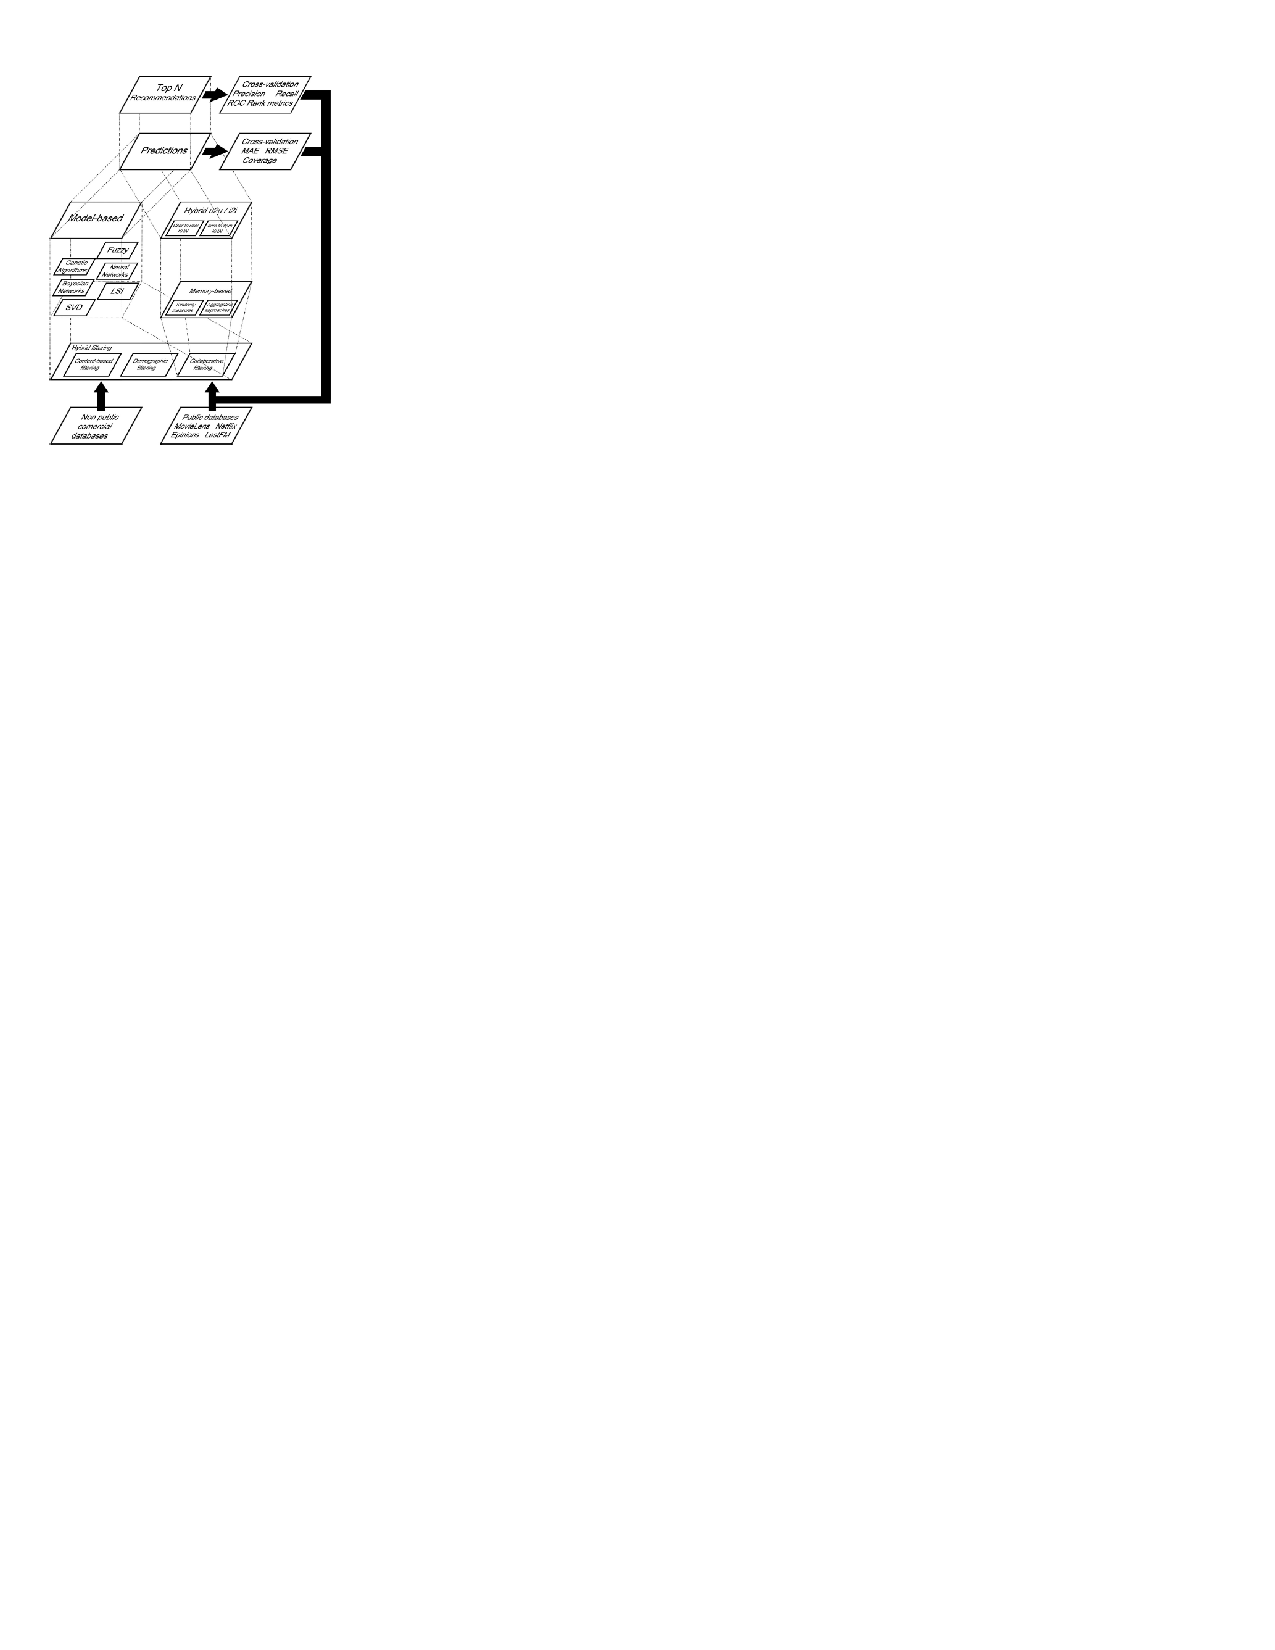
\includegraphics[width=0.70\textwidth]{Figure_1_8.pdf}
%  \caption{Các phương pháp khuyến nghị truyền thống, phổ biến}\label{fig:figure_1_8}
%  (Nguồn hình vẽ: \cite{Bobadilla2013109})
%\end{center}
%\end{figure}
\begin{figure}[ht]
\begin{center}
\advance\leftskip-3cm
\advance\rightskip-3cm
  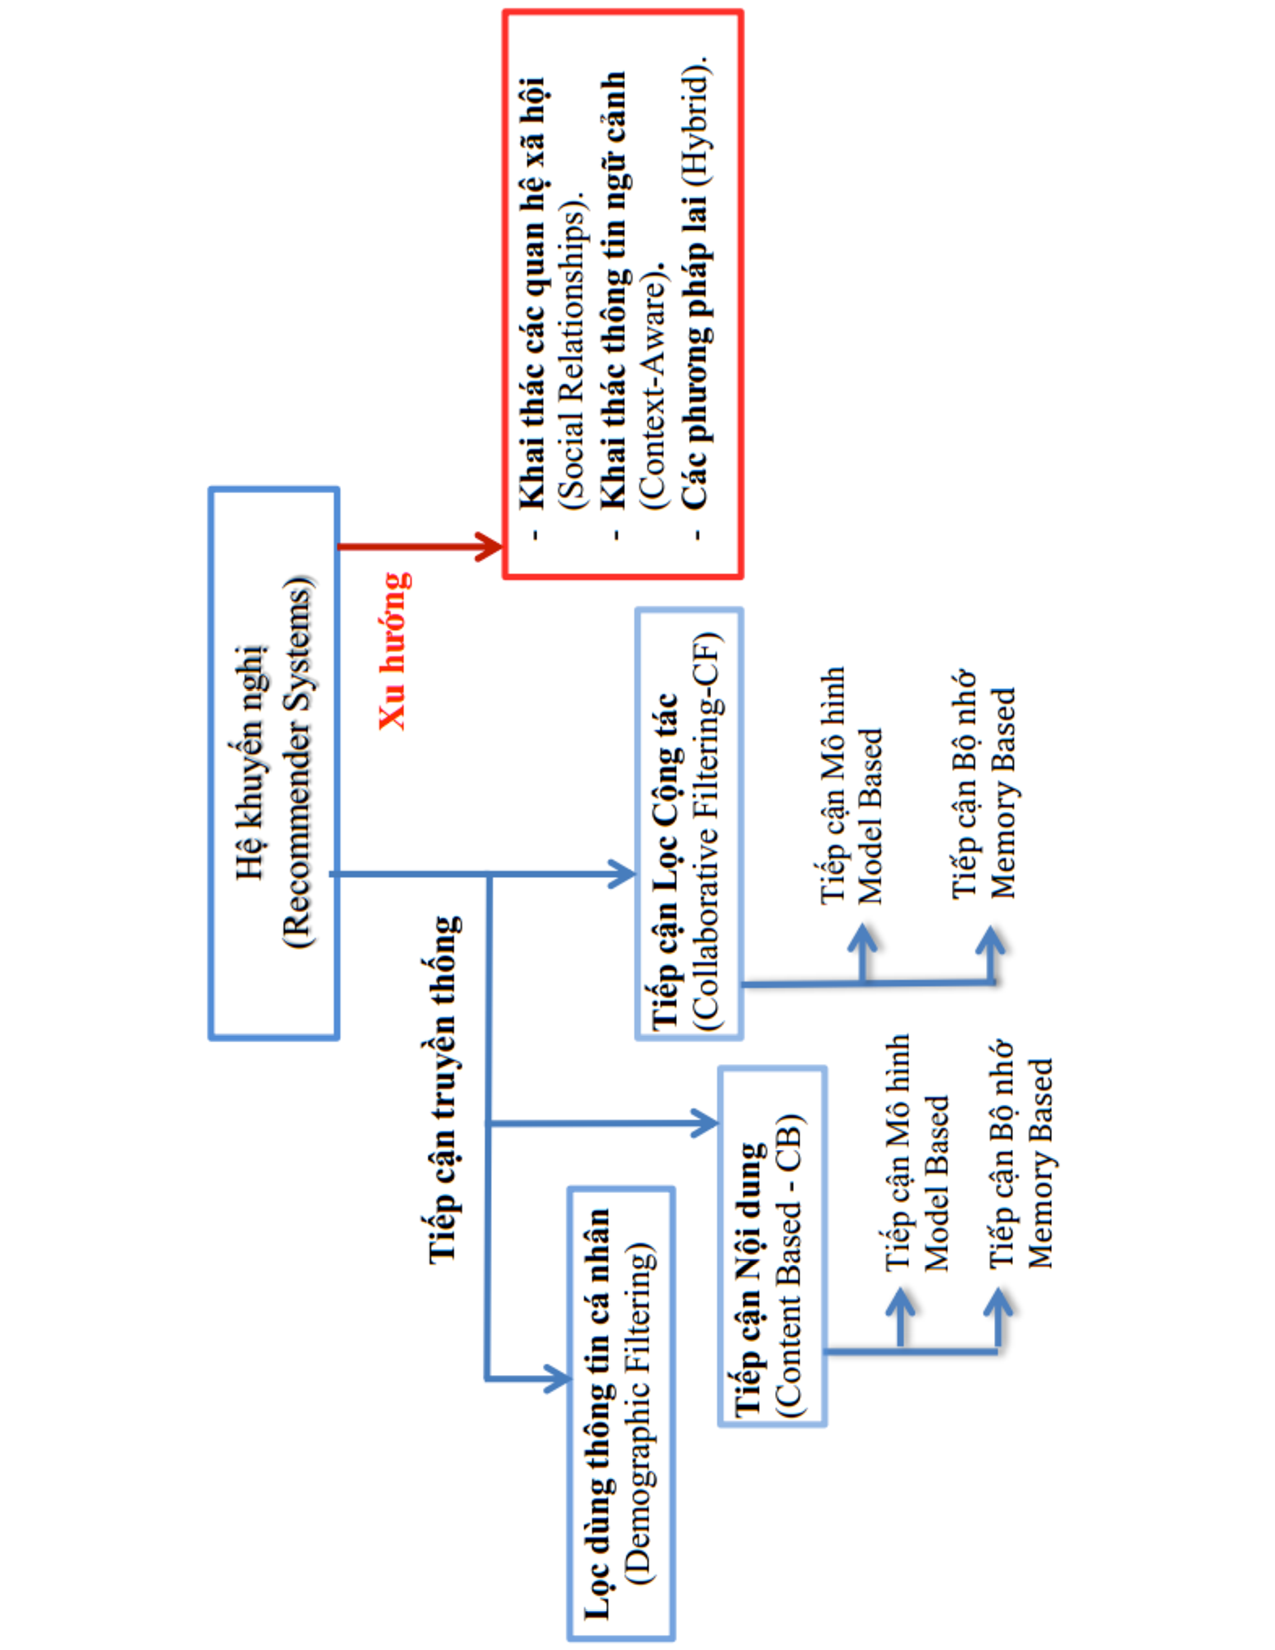
\includegraphics[width=0.99\textwidth]{Figure_1_7.pdf}
  \caption{Các cách tiếp cận phổ biến và xu hướng hiện nay cho hệ khuyến nghị}\label{fig:figure_1_7}
\end{center}
\end{figure}

%Bên cạnh việc phân loại hệ khuyến nghị theo cách tiếp cận, Bobadilla và cộng sự cũng đã phân loại hệ khuyến nghị dựa trên .... dữ liệu  
Bên cạnh đó, tác giả Bobadilla và cộng sự cũng đã khảo sát và chỉ ra xu hướng hiện nay cho hệ khuyến nghị \cite{Bobadilla2013109}. Hình \ref{fig:figure_1_7} thể hiện tóm tắt các cách tiếp cận truyền thống, phổ biến cũng như xu hướng hiện nay cho hệ khuyến nghị. Phân tiếp theo sẽ trình bày chi tiết, cũng như phân tích ưu điểm, hạn chế của một số tiếp cận chính trong phạm vi luận án.

\subsection{Tiếp cận nội dung (CB)}
\textbf{Định nghĩa 1.4:} \textit{Hồ sơ người dùng}

Hồ sơ người dùng $u$, ký hiệu là $UserProfile(u)$, biểu diễn sở thích của $u$ và giúp hệ khuyến nghị tiên đoán một đối tượng $p \in P$ có hữu ích hay không và mức độ hữu ích đối với $u$ là như thế nào. $UserProfile(u)$ có thể xây dựng từ việc phân tích đặc trưng các đối tượng khuyến nghị mà $u$ quan tâm, đánh giá trong quá khứ thông qua tương tác với hệ thống. \\

Tiếp cận nội dung có nguồn gốc từ cộng đồng nghiên cứu về truy vấn thông tin và lọc thông tin \cite{Belkin:1992, Balabanovic:1997:FCC}. Tiếp cận nội dung tìm cách khuyến nghị các đối tượng tương tự với những đối tượng mà người dùng quan tâm trong quá khứ. Chẳng hạn, nếu người dùng thường đọc các trang tin tức có chứa những từ như: Grand Slam, Roger Fedeger, Nadal, Djokovic, Australia Open, French Open, Wimbledon, US Open, v.v...  thì các trang chứa tin tức liên quan đến chủ đề tennis mà người dùng chưa biết sẽ được khuyến nghị cho người dùng. Một ví dụ khác, nếu một nghiên cứu viên thường tải, đọc hay viết những bài báo khoa học về IR thì các bài báo khoa học về IR mới, cập nhật mà nghiên cứu viên đó chưa biết sẽ được ưu tiên khuyến nghị.

Để ước lượng có hay không người dùng $u$ sẽ thích đối tượng khuyến nghị $p$ và thích nhiều hay ít (tức việc xây dựng và ước lượng giá trị hàm hữu ích $f(u,p)$), các phương pháp dựa trên tiếp cận nội dung thông thường sẽ thực hiện các bước sau:
\begin{itemize}
	\item Bước 1: Biểu diễn nội dung đối tượng khuyến nghị $p \in P$, ký hiệu ($Content(p)$).
	\item Bước 2: Mô hình hóa sở thích người dùng $u \in U$, gọi tắt là hồ sơ người dùng (User Profile), ký hiệu ($UserProfile(u)$). 
	\item Bước 3: Ước lượng giá trị hữu ích dựa trên độ tương tự nội dung của đối tượng khuyến nghị $p$ với hồ sơ người dùng $u$. Hệ thống sẽ ưu tiên khuyến nghị những đối tượng có nội dung tương tự cao so với hồ sơ người dùng $u$.
	\begin{equation}
	f(u,p) = Sim(UserProfile(u), Content(p))
	\end{equation}
\end{itemize}

\subsubsection{Kiến trúc hệ thống}
Pasquale Lops và cộng sự đã tiến hành khảo sát, phân tích các hệ khuyến nghị dựa trên tiếp cận nội dung \cite{Lops2011CBRecSys}. Theo Pasquale Lops và cộng sự, hệ khuyến nghị dựa trên tiếp cận nội dung thường sẽ thực hiện 3 việc chính và được đảm trách bởi ba thành phần tương ứng đó là: (1) Phân tích nội dung (Content Analyzer): có nhiệm vụ phân tích, mô hình hóa nội dung của các đối tượng khuyến nghị; (2) Mô hình hóa hồ sơ người dùng (Profile Learner): xây dựng và cập nhật hồ sơ người dùng dựa trên đặc trưng các đối tượng mà người dùng quan tâm, yêu thích; (3) Lọc nội dung (Filtering Component): thực hiện khuyến nghị dựa trên việc so khớp đặc trưng nội dung của đối tượng khuyến nghị với hồ sơ người dùng. Kiến trúc tổng quan của hệ khuyến nghị dựa trên tiếp cận nội dung thể hiện qua hình vẽ \ref{fig:figure_1_11}.
\begin{figure}[ht]
	\begin{center}
		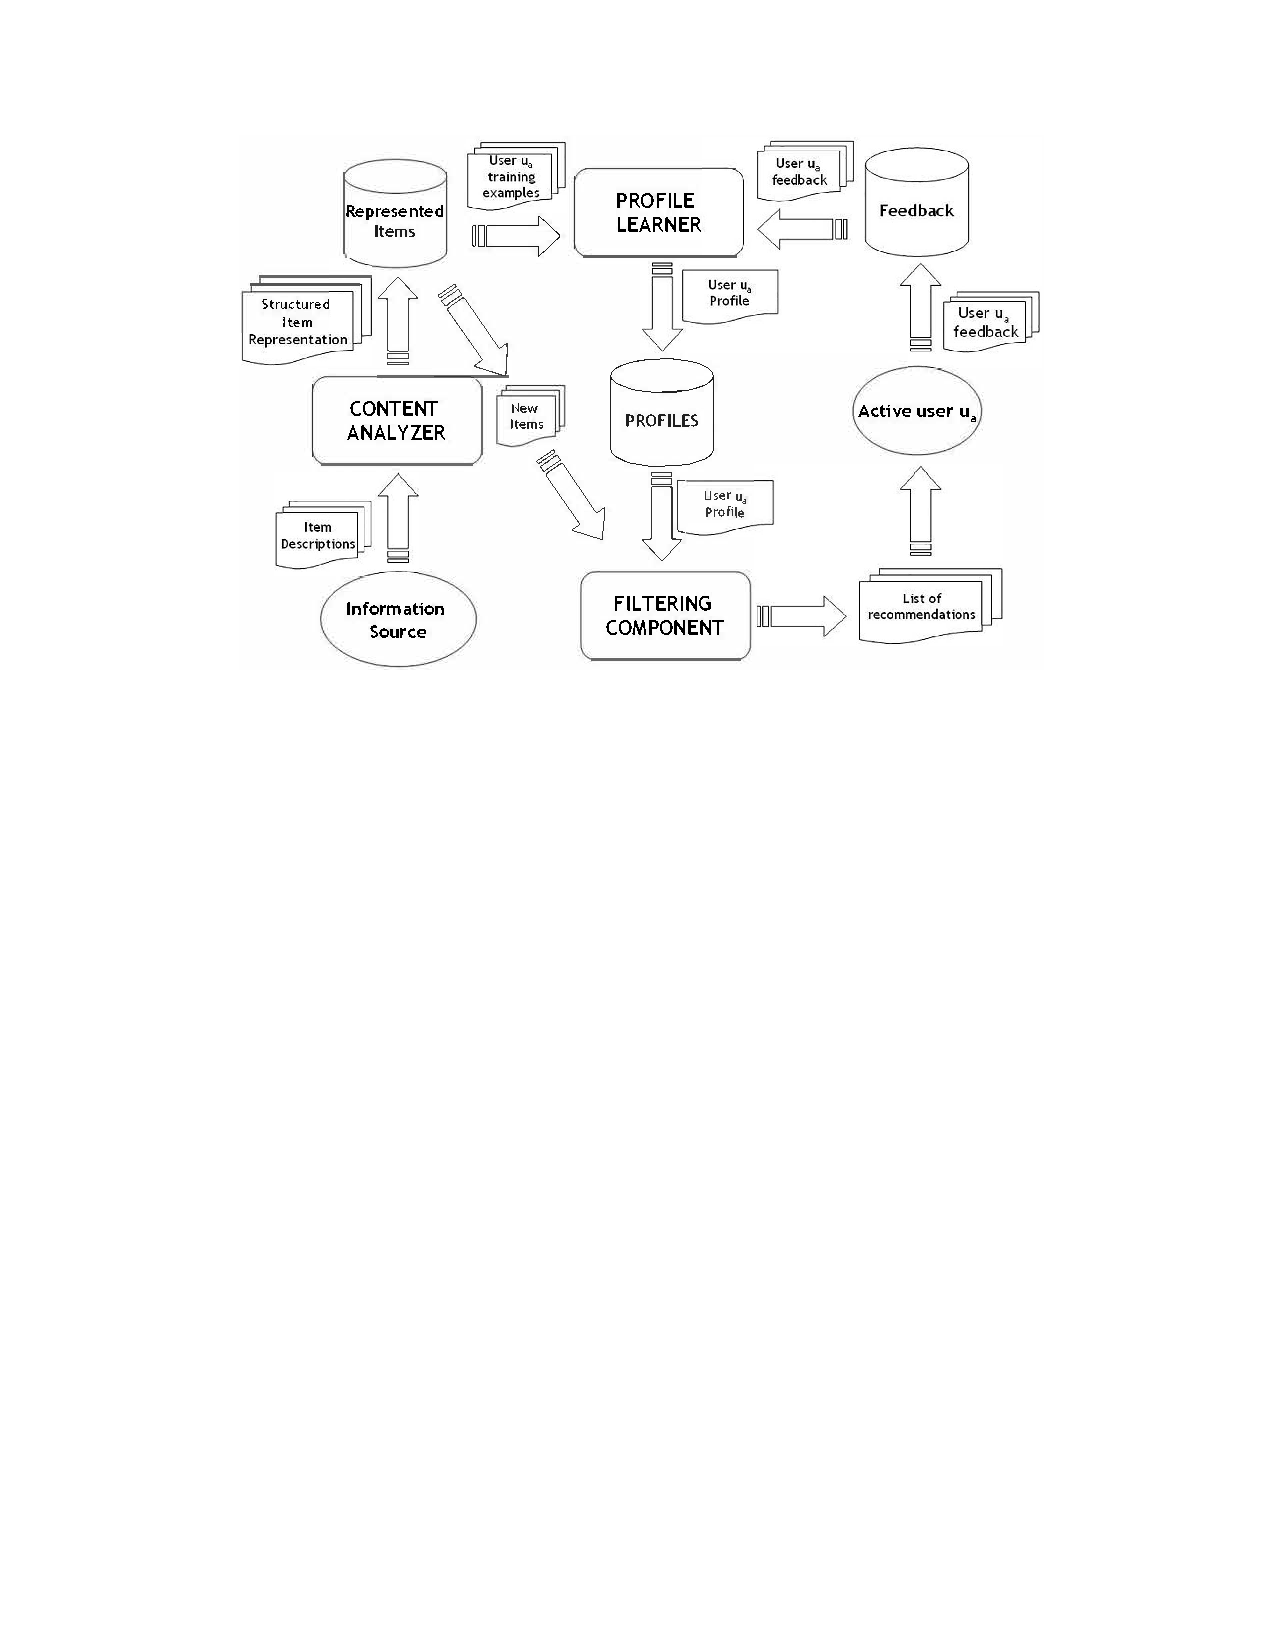
\includegraphics[width=0.9\textwidth]{Figure_1_11.pdf}
		\caption{Kiến trúc tổng quan của hệ khuyến nghị dựa trên tiếp cận nội dung}\label{fig:figure_1_11}
		(Nguồn hình vẽ: \cite{Lops2011CBRecSys})
	\end{center}
\end{figure}
\begin{itemize}
	\item \textbf{Phân tích nội dung (Content Analyzer):} thành phần này có nhiệm vụ phân tích và mô hình hóa nội dung của các đối tượng khuyến nghị. Tùy vào bài toán cụ thể, các phương pháp rút trích đặc trưng sẽ được dùng để chuyển nội dung đối tượng khuyến nghị từ định dạng gốc sang không gian đặc trưng. Trường hợp dữ liệu của đối tượng khuyến nghị là không cấu trúc (ví dụ tài liệu văn bản) thì các bước tiền xử lý như loại bỏ hư từ (stop word), chuyển về gốc từ (stemming) sẽ được tiến hành trước khi rút trích đặc trưng và mô hình hóa thành những vectơ từ khóa. Mô hình biểu diễn đối tượng khuyến nghị là đầu vào cho bước học, mô hình hóa hồ sơ người dùng và bước so khớp để thực hiện khuyến nghị.
	\item \textbf{Mô hình hóa hồ sơ người dùng (Profile Learner):} các nghiên cứu thường dùng các phương pháp học máy giám sát để học hồ sơ người dùng dựa trên đặc trưng của các đối tượng mà người dùng thích hay không thích trong quá khứ. Qua thời gian sở thích người dùng có thể thay thay đổi. Dựa trên dữ liệu phản hồi rõ ràng hay tiềm ẩn của người dùng thông qua tương tác với hệ thống, hệ thống thường sẽ định kỳ để học và cập nhật lại hồ sơ người dùng.
	\item \textbf{Lọc nội dung (Filtering Component):} thành phần này có nhiệm vụ so khớp hồ sơ người dùng với nội dung của các đối tượng để thực hiện khuyến nghị những đối tượng phù hợp với sở thích người dùng. Kết quả so khớp sẽ thể hiện mức độ quan tâm của người dùng $u\in U$ lên đối tượng khuyến nghị $p\in P$. Nói cách khác, giá trị hàm hữu ích $f(u,p)$ của sản phẩm $p$ với người dùng $u$ được ước lượng dựa trên độ tương tự nội dung của đối tượng khuyến nghị $p \in P$ với nội dung các đối tượng $p' \in P$, $\{p'\}$ là tập các đối tượng liên quan đến $u$ hay được $u$ quan tâm trong quá khứ. 
\end{itemize}

Một trong những vấn đề ảnh hưởng đến hiệu năng của tiếp cận nội dung là kỹ thuật phân tích nội dung và phương pháp mô hình hóa hồ sơ người dùng. 

\subsubsection{Xây dựng và cập nhật hồ sơ người dùng}
Hồ sơ người dùng giúp hệ thống có thể hiểu được sở thích của người dùng và tiên đoán một đối tượng có hữu ích hay không và mức độ hữu ích đối với mỗi người dùng là như thế nào. Có thể nói hồ sơ người dùng là yếu tố then chốt quyết định hiệu quả của các hệ khuyến nghị dựa trên nội dung. Vấn đề đặt ra là làm thế nào để có thể ghi nhận thông tin sở thích của người dùng và làm thế nào để mô hình hóa, cập nhật hồ sơ người dùng trong các hệ khuyến nghị dựa trên nội dung? Phần tiếp theo sẽ giúp chúng ta trả lời những cầu hỏi này.

\subsubsection*{(*) Thông tin phản hồi của người dùng}
Thông qua những phản hồi thì hệ thống có thể biết được những đối tượng nào được người dùng quan tâm và mức độ là nhiều hay ít. Susan Gauch và đồng nghiệp \cite{Gauch:2007}, cũng như Pasquale Lops và đồng nghiệp \cite{Lops2011CBRecSys}, đã phân thông tin phản hồi của người dùng thành hai loại: rõ ràng và tiềm ẩn khi người dùng tương tác với hệ thống. Những hình thức phản hồi rõ ràng của người dùng như: nhập trực tiếp vào hệ thống những từ khóa thể hiện sở thích, nhấn chọn thích hay không hoặc cho những điểm đánh giá trong một khoảng nào đó (thường từ 1 đến 5), đưa ra những bình luận đối với những đối tượng mà hệ thống khuyến nghị. Tuy nhiên, trên thực tế chỉ một số lượng rất ít người dùng chia sẻ những thông tin, quan điểm của họ về những đối tượng khuyến nghị khi sử dụng và tương tác với hệ thống. Vì vậy, nhiều hệ thống đã tìm cách ghi nhận thông tin phản hồi tiềm ẩn bằng việc phân tích hành vi sử dụng hệ thống của người dùng thông qua bộ nhớ đệm của trình duyệt, tập tin log, v.v... Những phản hồi tiềm ẩn có thể kể đến như: chọn xem, đánh dấu và lưu trang, thời gian xem, v.v... 

Thông thường, hệ thống sẽ mô hình hóa hồ sơ người dùng dựa trên thông tin phản hồi và nội dung đối tượng. Nội dung của đối tượng khuyến nghị thường được biểu diễn bởi một tập các đặc trưng. Chẳng hạn, đối tượng là bài báo khoa học thì có thể biểu diễn bởi một số đặc trưng cơ bản như: tác giả, hội thảo, tạp chí, từ khóa thể hiện chủ đề bài báo, v.v... Tùy vào bài toán cụ thể thì các phương pháp rút trích đặc trưng sẽ được dùng để chuyển nội dung đối tượng khuyến nghị từ định dạng dữ liệu gốc sang không gian đặc trưng. 

\subsubsection*{(*) Mô hình hóa hồ sơ người dùng}
Hầu hết các hệ khuyến nghị nội dung áp dụng mô hình truy vấn đơn giản như so khớp từ khóa hoặc mô hình không gian vectơ. Đặc trưng của đối tượng thường là các đặc trưng dạng văn bản được rút trích từ các trang web, nội dung bài báo, thông tin mô tả sản phẩm. Trường hợp dữ liệu của đối tượng khuyến nghị là không cấu trúc, chẳng hạn tài liệu văn bản, thì các bước tiền xử lý như loại bỏ hư từ (stop word), chuyển về gốc từ (stemming) sẽ được tiến hành trước khi rút trích đặc trưng và mô hình hóa thành những vectơ từ khóa. Mô hình biểu diễn nội dung đối tượng khuyến nghị là đầu vào cho bước học hồ sơ người dùng và bước so khớp để thực hiện khuyến nghị. 

Với mô hình không gian vectơ thì nội dung của đối tượng khuyến nghị $p \in P$, ký hiệu là $Content(p)$, được biểu diễn dưới dạng một vectơ đặc trưng như sau:
\begin{equation}
	Content(p) = \overrightarrow{w_{p}} = (w_{1,p}, w_{2,p}, ..., w_{k,p})
\end{equation}
Trong đó, 
\begin{itemize}
	\item $k$: là tổng số đặc trưng dùng để biểu diễn nội dung đối tượng. Đơn giản nhất là từ điển các từ khóa sau khi loại bỏ các stop word và thực hiện stemming.
	\item $w_{i,p}$ trọng số đặc trưng thứ $i$ của đối tượng $p$.
\end{itemize}

Trọng số mỗi chiều trong vectơ $\overrightarrow{w_{u}}$ và $\overrightarrow{w_{p}}$ có thể ước lượng dựa trên tần suất xuất hiện của từ khóa bằng phương pháp TFIDF \cite{Baeza-Yates:1999:MIR}.

Hồ sơ người dùng thường được xây dựng dựa trên nội dung của các đối tượng mà họ thể hiện sự quan tâm, đánh giá khi tương tác, sử dụng hệ thống. Như vậy, với $k$ đặc trưng biểu diễn nội dung các đối tượng khuyến nghị, hồ sơ người dùng $u$ có thể biểu diễn dưới dạng một vectơ đặc trưng cũng với số chiều là $k$ như sau:
\begin{equation}
UserProfile(u) = \overrightarrow{w_{u}} = (w_{1,u}, w_{2,u}, ..., w_{k,u})
\end{equation}

Trong đó, 
\begin{itemize}
	\item $w_{i,u}$ trọng số đặc trưng thứ $i$ trong hồ sơ người dùng $u$.
\end{itemize}

Việc ước lượng giá trị hàm hữu ích thông thường có thể dùng độ đo cosine trong truy vấn thông tin \cite{Baeza-Yates:1999:MIR}.
\begin{equation}
f(u,p) = Cosine(\overrightarrow{w_{u}},\overrightarrow{w_{p}}) = 
\frac{\overrightarrow{w_{u}} \bullet \overrightarrow{w_{p}}}{\parallel \overrightarrow{w_{u}} \parallel \ast \parallel \overrightarrow{w_{p}}\parallel}
\end{equation}
Trong đó: dấu $\bullet$ thể hiện tích hai vectơ, dấu $\ast$ thể hiện tích vô hướng và $\parallel.\parallel$ là độ dài của vectơ.

Nhiều hệ thống khuyến nghị nội dung dựa trên từ khóa đã được nghiên cứu và phát triển trong nhiều lĩnh vực ứng dụng khác nhau như: khuyến nghị phim, khuyến nghị web, khuyến nghị tin tức, v.v... Trong tài liệu \cite{Lops2011CBRecSys}, Pasquale Lops và cộng sự cũng đã tiến hành khảo sát và phân tích các hệ thống khuyến nghị tin tức. Đối với các hệ thống này thì hồ sơ người dùng sẽ được học dựa trên nội dung các trang mà người dùng phản hồi quan tâm hay không quan tâm. Một số nghiên cứu tìm cách mô hình hóa sở thích dài hạn của người dùng như hệ thống khuyến nghị tin NewsT \cite{366590}, YourNews \cite{Ahn:2007}. Bên cạnh đó, một số nghiên cứu khác như Daily Learner \cite{Billsus:2000:UMA:598285.598352}, NewsDude \cite{Billsus:1999:HUM:317328.317338}, thì xây dựng hai mô hình sở thích cho mỗi người dùng: mô hình sở thích dài hạn và mô hình sở thích ngắn hạn. 

Trong lĩnh vực khuyến nghị trang web, tác giả Henry Lieberman đã đề xuất một hệ thống Letizia, hỗ trợ người dùng duyệt web \cite{Lieberman:1995}. Letizia có thể làm việc với các trình duyệt để lưu vết hành vi duyệt web của người dùng. Hệ thống sẽ xây dựng hồ sơ người dùng dựa trên các từ khóa rút trích từ những trang mà người dùng quan tâm. Henry Lieberman xem xét sở thích của người dùng thông qua các phản hồi tiềm ẩn, chẳng hạn hành vi lưu, đánh dấu một trang. Tương tự vậy, Dunja Mladenic đã nghiên cứu phát triển hệ thống Personal WebWatcher nhằm hỗ trợ người dùng duyệt web. Personal WebWatcher sẽ làm nổi bậc các liên kết tiềm năng trong các trang web mà người dùng duyệt qua. Tác giả đã dùng phương pháp học máy giám sát để học sở thích người dùng dựa trên nội dung các liên kết mà người quan tâm (nhấn chuột) và không quan tâm \cite{mladenic99acai}.

Nói chung, hầu hết những hệ thống khuyến nghị nội dung thực hiện mô hình hóa nội dung đối tượng dựa trên mô hình không gian vectơ với đặc trưng từ khóa và học mô hình người dùng dựa trên những phản hồi, tương tác rõ ràng hay tiềm ẩn của người dùng với hệ thống. Việc dùng đặc trưng từ khóa để biểu diễn nội dung đối tượng và xây dựng hồ sơ người dùng thường gặp phải một số vấn đề khó khăn liên quan đến xử lý ngôn ngữ tự nhiên như: khác âm đồng nghĩa (synonymy), đồng âm khác nghĩa (polysemy). Để giải quyết những hạn chế liên quan đến việc mô hình hóa nội dung đối tượng dựa trên từ khóa, một số nghiên cứu khác quan tâm đến việc phát triển các phương pháp biễu diễn nội dung đối tượng và hồ sơ người dựa trên mô hình mạng ngữ nghĩa hoặc đặc trưng khái niệm thay vì đặc trưng từ khóa.

%\subsubsection*{(*) Mô hình ngữ nghĩa}
%Tiếp cận mô hình hóa dựa trên ngữ nghĩa thường sử dụng các cơ sở tri thức, từ điển ngôn ngữ, ontologies. Trong tài liệu \cite{Gauch:2007}, các tác giả đã tiến hành khảo sát, phân tích các phương pháp khác nhau để mô hình hóa hồ sơ người dùng trong cho các hệ thống thông tin cá nhân. Các tác giả đã phân tích việc mô hình hóa hồ sơ người dùng bằng mô hình mạng ngữ nghĩa hoặc dùng đặc trưng khái niệm thay vì từ khóa. 
%
%Để giải quyết những vấn đề nhập nhằng ngữ nghĩa trong xử lý ngôn ngữ tự nhiên, nhiều nghiên cứu đã tìm cách biểu diễn hồ sơ người dùng dựa trên mạng ngữ nghĩa có trọng số với nút là một khái niệm và cung là sự đồng hiện của hai khái niệm liên quan. Trọng số của nút và cung thể hiện mức độ quan tâm của người dùng lên những khái niệm tương ứng. Việc tính toán giá trị hữu ích dùng các kỹ thuật so khớp trên mạng ngữ nghĩa với đầu vào là các khái niệm biểu diễn ngữ nghĩa đối tượng khuyến nghị và mạng ngữ nghĩa của người dùng. Trong dự án SiteIF \cite{Stefani1998}, các tác giả dùng Wordnet để gom những từ liên quan đến một khái niệm, gọi là synsets (synonym sets) và mỗi nút trong mạng là một synsets. Tương tự vậy, hệ thống InfoWeb cũng dùng một mạng có trọng số các khái niệm để mô hình hóa sở thích dài hạn của người dùng nhằm hỗ trợ tốt hơn khi người dùng tìm kiếm tài liệu trong thư viện số \cite{Gianluigi-Gentili-2003}.

\subsubsection*{(*) Cập nhật hồ sơ người dùng}  
Trên thực tế, sở thích của người dùng thường sẽ thay đổi theo thời gian. Tùy vào lĩnh vực ứng dụng, mà sở thích người dùng sẽ thay đổi nhanh hay chậm. Chẳng hạn, trong lĩnh vực khuyến nghị phim, sách hay bài báo khoa học thường thì sở thích người dùng sẽ thay đổi chậm hơn so với lĩnh vực khuyến nghị tin tức. Trong khuyến nghị tin tức, đôi khi người dùng cần đọc những tin quan trọng, "nóng" mà không thuộc chủ đề họ quan tâm (tức không liên quan đến sở thích người dùng). Do đó, vấn đề thay đổi sở thích của người dùng là một trong những khó khăn, thách thức ảnh hưởng đến việc xây dựng và cập nhật hồ sơ người dùng trong các hệ khuyến nghị dựa trên nội dung. 

Để đương đầu với sự thay đổi sở thích của người dùng, nhiều nghiên cứu đã đề xuất các giải pháp khác nhau cho việc xây dựng và cập nhật hồ sơ người dùng. Một số nghiên cứu liên quan đến khuyến nghị tin tức tìm cách mô hình hóa hồ sơ người dùng thành hai phần: sở thích dài hạn (thay đổi chậm) và sở thích ngắn hạn (thanh đổi nhanh) như: Daily Learner \cite{Billsus:2000:UMA:598285.598352}, NewsDude \cite{Billsus:1999:HUM:317328.317338}. Saranya.K.G và Sadhasivam đề xuất hai loại hồ sơ người dùng là: tĩnh (bao gồm thông tin do người dùng đăng ký) và động được xây dựng dựa trên thông tin tiềm ẩn mà người dùng tương tác với hệ thống. Trong lĩnh vực E-Learning, Nguyen và đồng nghiệp \cite{nguyentool}, Le và đồng nghiệp \cite{Le-ELearningSys}, đã nghiên cứu phát triển phương pháp xây dựng và cập nhật hồ sơ người dùng dựa trên luật, ứng dụng vào hệ khuyến nghị tài nguyên, dịch vụ dạy và học trong E-Learning. Các tác giả đã đề xuất mô hình $\alpha$-Community để xây dựng và cập nhật hồ sơ người học dựa trên luật. Mô hình $\alpha$-Community dựa trên lý thuyết tập thô và ý tưởng cơ bản là giá trị đặc trưng của hồ sơ người học sẽ được suy diễn dựa trên hồ sơ của những thành viên trong cùng nhóm học tập, cộng đồng. 
%thông tin phản hồi rõ ràng và tiềm ẩn của sinh viên thường không chính xác, đủ tin cậy để xây dựng hồ sơ người học vì sinh viên thường chỉ thể hiện là thích hay không và nhiều hay ít đối với một môn học, tài liệu nào đó chư họ không đủ kiến thức để biết được chủ đề, môn học, tài liệu nào là cần thiết, hữu ích đối với họ. Xác định một số khó khăn, thách thức đối với việc xây dựng và cập nhật hồ sơ người học trong lĩnh vực E-Learning, Nguyễn và đồng nghiệp đã đề xuất mô hình \alpha-Community để xây dựng và cập nhật hồ sơ người học dựa trên luật. Mô hình \alpha-Community dựa trên lý thuyết tập thô và ý tưởng cơ bản là giá trị đặc trưng của hồ sơ người học sẽ được suy diễn dựa trên hồ sơ của những thành viên trong cùng nhóm học tập, cộng đồng \cite{Le-ELearningSys}. 

Tóm lại, mỗi bài toán, lĩnh vực ứng dụng sẽ có phương pháp phù hợp để xây dựng và cập nhật hồ sơ người dùng. Với những lĩnh vực mà sở thích người dùng thay đổi nhanh thì có thể chia hồ sơ người dùng thành 2 phần: tĩnh (dài hạn) và động (ngắn hạn). Thông thường, các hệ khuyến nghị sẽ định thời để cập nhật lại hồ sơ người dùng qua một khoảng thời gian. Hình \ref{fig:figure_1_12} minh họa các bước cơ bản liên quan việc học và cập nhật hồ sơ người dùng.
\begin{figure}[ht]
	\begin{center}
		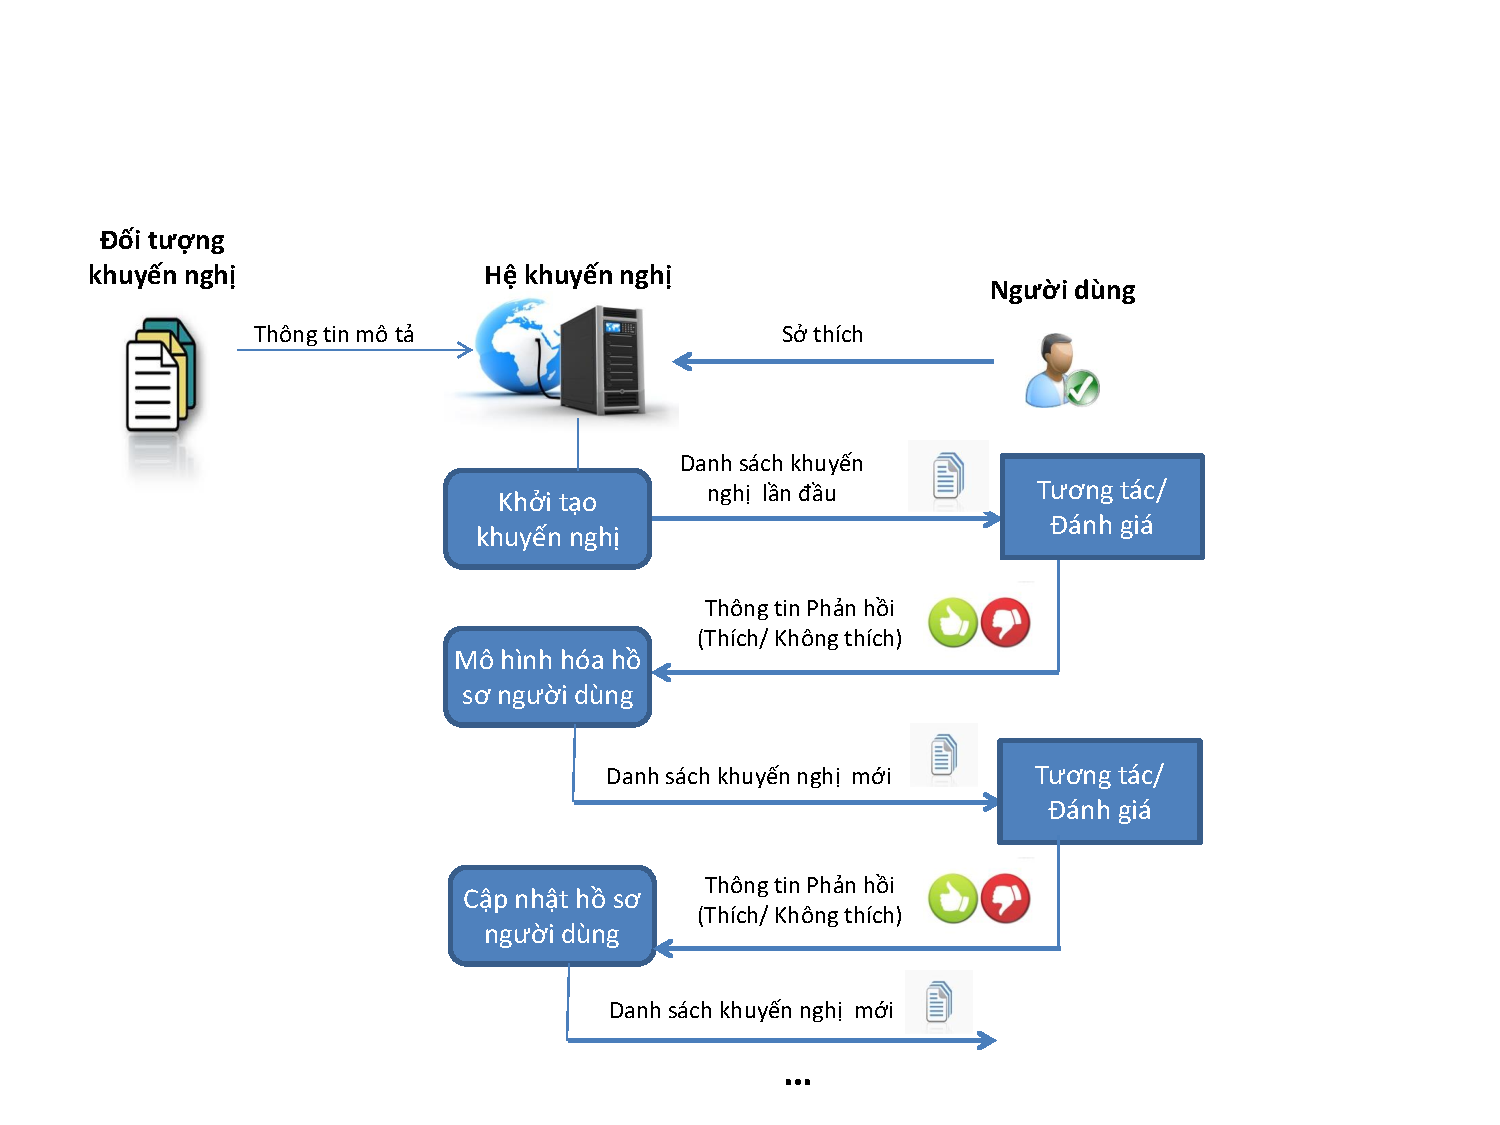
\includegraphics[width=0.70\textwidth]{Figure_1_12.pdf}
		\caption{Học và cập nhật hồ sơ người dùng dựa trên thông tin phản hồi}\label{fig:figure_1_12}
	\end{center}
\end{figure}
\subsubsection{Phân loại tiếp cận nội dung}
Các phương pháp truyền thống dựa trên nội dung có thể chia thành hai nhóm chính: (1) Một là các phương pháp dựa trên bộ nhớ, thực hiện tính toán độ tương tự và khoảng cách giữa $Content(p)$ và $UserProfile(u)$ dùng các độ đo Cosine, Euclide \cite{Baeza-Yates:1999:MIR}; (2) Hai là các phương pháp dựa trên mô hình, với mô hình được học từ dữ liệu dùng các kỹ thuật học máy để phân các đối tượng khuyến nghị thành những đối tượng người dùng quan tâm (1) hay không quan tâm (0) như: phân lớp SVM \cite{Joachims:1998:TCS}, phân lớp Bayesian \cite{Nigam:2000:TCL} và các phương pháp xác suất như: Pazzani và Billsus \cite{Pazzani:1997}, Mooney và Roy \cite{Mooney:2000:CBR}, Gemmis và đồng nghiệp \cite{deGemmis:2008:ITS}. Chẳng hạn phân lớp Bayesian có thể dùng để ước lượng xác suất một tài liệu (đối tượng khuyến nghị $p$) thuộc lớp $C_{x}$ (quan tâm và không quan tâm), khi cho trước một tập các từ khóa mô tả tài liệu $p$ này là $\{k_{1,p}, k_{2,p}, ..., k_{n,p}\}$, chính là $P(C_{x}|k_{1,p}, k_{2,p}, ..., k_{n,p})$ \cite{Nigam:2000:TCL}.

\subsubsection*{(a) Tiếp cận nội dung dựa trên bộ nhớ}
Tiếp cận nội dung dựa trên bộ nhớ thường thực hiện việc ước lượng mức độ hữu ích của đối tượng khuyến nghị $p \in P$ với người dùng $u \in U$ (tức giá trị hàm hữu ích $f(u,p)$) dựa trên việc tổng hợp mức độ quan tâm của $u$ đối với tập $k$ đối tượng có nội dung tương tự với $p$, ký hiệu $P_{k} = \{p_{k}\}, P_{k} \subseteq P$, hoặc tổng hợp mức độ quan tâm từ tập $k$ những người dùng có sở thích tương tự $u$, $U_{k} = \{u_{k}\}, U_{k} \subseteq U$. Tùy thuộc vào cách biểu diễn nội dung đối tượng dữ liệu và hồ sơ người dùng, chúng ta sẽ có một hàm phù hợp để tính độ tương tự và xác định tập $P_{k}$, cũng như $U_{k}$. Thông thường, các nghiên cứu dùng mô hình không gian vectơ và độ đo Cosine để biểu diễn nội dung và tính độ tương tự giữa các đối tượng. 

Phương pháp dựa trên bộ nhớ được nhiều nghiên cứu sử dụng là phương pháp lân cận gần nhất, kNN. Để phát triển hệ thống khuyến nghị tin tức, Daniel Billsus và Michael J. Pazzani đã dùng phương pháp kNN xây dựng hồ sơ người dùng ngắn hạn kết hợp với hồ sơ người dùng dài hạn được xây dựng dùng phương pháp Bayesian \cite{Billsus:2000:UMA:598285.598352}. Các tác giả đã chỉ ra rằng, việc chia hồ sơ người dùng thành hai phần giúp biểu diễn đa dạng hơn sở thích của người dùng. Trong nghiên cứu của họ, kNN được dùng để xác định chuỗi tất cả các tin tức liên quan đến một sự kiện nào đó dựa trên độ tương tự nội dung với một số tin mà người dùng quan tâm, đánh giá. Việc mô hình sở thích ngắn hạn dùng kNN sẽ dễ dàng thích nghi với những quan tâm mới của người dùng trong một khoảng thời gian ngắn, thay vì hệ thống phải cần rất nhiều dữ liệu huấn luyện để xây dựng lại toàn hồ sơ người dùng sử dụng các phương pháp học máy. Việc xác định người dùng tương tự dựa trên ma trận đánh giá thường gặp phải một số vấn đề ảnh hưởng đến độ chính xác như: ma trận đánh giá thưa, một số người dùng có chung đánh giá cho cùng đối tượng nhưng vì những lý do khác nhau. Do đó, Maria Terzi và cộng sự đã đề xuất dùng kNN để xác định nhóm những người dùng tương tự dựa trên nội dung bình luận về các đối tượng khuyến nghị (Text-based User-kNN) thay vì dựa trên sự tương quan trong ma trận đánh giá \cite{TerziMaria2014}. Các tác giả đã tiến hành thực nghiệm trên tập dữ liệu phim từ RottenTomatoes\footnote{http://www.rottentomatoes.com/} và tập đĩa nhạc từ Amazon\footnote{https://www.amazon.com/}. Kết quả thực nghiệm cho thấy phương pháp tương tự người dùng dựa trên nội dung bình luận cho kết quả tốt hơn việc xác định người dùng dựa trên ma trận đánh giá. Tương tự, các tác giả Li Chen và Feng Wang \cite{ChenW13}, Claudiu Cristian Musat và cộng sự \cite{MusatLF13}, cũng tiến hành xây dựng hồ sơ người dùng dựa trên nội dung văn bản rút trích từ các đối tượng mà người dùng quan tâm, đánh giá để xác định nhóm những người dùng tương tự thay vì dựa trên ma trận đánh giá. Nhìn chung, các phương pháp dựa trên bộ nhớ có những ưu điểm và hạn chế sau:\\
\textbf{Ưu điểm:}
\begin{itemize}
	\item Chất lượng khuyến nghị thường sẽ tốt hơn do tính toán trên cả tập dữ liệu khi thực hiện khuyến nghị.
	\item Đơn giản, dễ hiện thực.
\end{itemize}	
\textbf{Hạn chế:}
\begin{itemize}
	\item Tốn bộ nhớ và tốc độ xử lý chậm do phải tính toán trên cả tập dữ liệu khi thực hiện khuyến nghị.
	\item Không thể tổng quát hóa tập dữ liệu.
\end{itemize}	

\subsubsection*{(b) Tiếp cận nội dung dựa trên mô hình}
Với các phương pháp dựa trên bộ nhớ, hệ thống thường sẽ tính giá trị hàm hữu ích dựa trên các độ đo như Cosine, Euclide. Đối với các phương pháp dựa trên mô hình, một mô hình sẽ được huấn luyện từ dữ liệu để phân các đối tượng khuyến nghị thành những đối tượng được người dùng quan tâm (1) hay không quan tâm (0) và quan tâm nhiều hay ít dùng các phương pháp học máy giám sát: phân lớp SVM \cite{Joachims:1998:TCS}, phân lớp Bayesian \cite{Nigam:2000:TCL} và một số các phương pháp xác suất khác. Nói cách khác, mô hình huấn luyện giúp tiên đoán giá trị hàm hữu ích $f(u,p)$ của đối tượng khuyến nghị $p \in P$ đối với người dùng $u \in U$. Chẳng hạn, phân lớp Bayesian là một phương pháp dựa trên mô hình khá phổ biến, được dùng trong khai thác dữ liệu, phân lớp Bayesian có thể dùng để ước lượng xác suất một đối tượng khuyến nghị $p$ hữu ích với $u$ như thế nào. Hay nói cách khác, $p$ được $u$ quan tâm hay không và quan tâm nhiều hay ít.

Ví dụ, xác suất một tài liệu $p$ được một người dùng $u$ nào đó quan tâm là bao nhiêu? Tức là, giá trị hàm hữu ích $f(u,p)$ khi đó sẽ được tính dựa trên việc ước lượng xác suất $p$ thuộc lớp $C_{1}(u)$ và $C_{0}(u)$  ($u$ quan tâm và không quan tâm đến $p$) là bao nhiêu, khi cho trước một tập các từ khóa mô tả tài liệu $p$ là $\{k_{1,p}, k_{2,p}, ..., k_{n,p}\}$. Giá trị hàm hữu ích $f(u,p)$ khi đó sẽ được tính như sau:
\begin{equation}
f(u,p) = P(p \in C_{1}(u)) = P(C_{1}(u)|k_{1,p}, k_{2,p}, ..., k_{n,p})
\end{equation}

Giả sử các từ khóa mô tả tài liệu là độc lập, khi đó xác suất $P(p \in C_{1}(u))$ sẽ là:
\begin{equation}
P(p \in C_{1}(u)) = P(C_{1}(u)|k_{1,p}, k_{2,p}, ..., k_{n,p}) = P(C_{1}(u))\prod_{i=1}^{n}P(k_{i,p}|C_{1}(u))
\end{equation}

Michael Pazzani và đồng nghiệp đã dùng tiếp cận dựa trên mô hình để phát triển hệ thống khuyến nghị các trang web phù hợp với sơ sở thích người dùng, Syskill \& Webert \cite{PazzaniMB96}. Các tác giả đã dùng một số phương pháp học máy truyền thống để xây dựng hồ sơ người dùng từ thông tin phản hồi của người dùng khi tương tác với hệ thống. Kết quả thực nghiệm của họ cho thấy việc ứng dụng phân lớp Bayesian để xây dựng hồ người dùng cho kết quả tốt hơn so với một số phương pháp khác như lân cận gấn nhất, mạng lan truyền ngược, cây quyết định. Trong bài báo \cite{liu2010personalized}, Jiahui Liu và cộng sự đã giới thiệu việc phát triển hệ thống khuyến nghị tin tức Google News. Hệ thống đã phân tích tập tin log để tìm hiểu sở thích, hành vi đọc tin của người dùng. Dựa trên kết quả phân tích, Jiahui Liu đã dùng phương pháp Bayesian để mô hình hóa hồ sơ người dùng và kết hợp với phương pháp lọc cộng tác để thực hiện khuyến nghị tin tức cho người dùng. Kết quả thực nghiệm của họ cho thấy, phương pháp đề xuất đã cải tiến chất lượng khuyến nghị tin tức, gia tăng, thu hút người dùng đến với trang Google News nhiều hơn. Nhìn chung, các phương pháp dựa trên mô hình có những ưu điểm và hạn chế sau:\\
%Tiếp cận nội dung thường được ứng dụng cho các bài toán mà nội dung đối tượng khuyến nghị thường được mô tả dưới dạng các từ khóa như tài liệu văn bản, các trang web. Các nghiên cứu, ứng dụng phổ biến dựa trên tiếp cận nội dung có thể kể đến như: các hệ thống khuyến nghị trang web cho người dùng Syskill \& Webert \cite{Pazzani:1997}, Fab \cite{Balabanovic:1997:FCC}; Hệ thống khuyến nghị phim, video phổ biến Youtube \cite{Davidson:2010:YoutubeRecSys}, MOVIES2GO \cite{Mukherjee:2001:MOV:375735.376018}; Các hệ thống khuyến nghị tin tức YourNews \cite{Ahn:2007:OUP:1242572.1242575}, PSUN \cite{Sorensen_psun:a}; Các nghiên cứu phát triển các hệ khuyến nghị việc làm dựa trên so khớp nội dung thông tin tuyển dụng và hồ sơ người tìm việc \cite{Malinowski:2006:MatchingPepoleJob, ZhengSiting:2012:JobRecSys, Lu:2013:RSJ}. Hệ thống định hướng tìm kiếm bài báo liên quan dựa trên thông tin đồng trích dẫn Citeseer \cite{Giles:1998:CiteSeer}. Một số các nghiên cứu nổi bật về khuyến nghị bài báo khoa học trong thời gian gần đây: Sugiyama và Kan \cite{Sugiyama:2010, Sugiyama:2011, Sugiyama:2013}, Huynh và đồng nghiệp \cite{Tin:Huynh:ResearchPaperRecommendation:2012}.
\textbf{Ưu điểm:}
\begin{itemize}
	\item Nhanh hơn so với các phương pháp dựa trên bộ nhớ do không phải tính trên cả tập dữ liệu mà chỉ dựa trên mô hình đã xây dựng để khuyến nghị.
	\item Khả năng đáp ứng tốt khi kích thước tập dữ liệu gia tăng.
	\item Một mô hình giúp biểu diễn tốt thế giới thực sẽ giúp tránh được vấn đề quá khớp (overfitting) so với các phương pháp dựa trên bộ nhớ.
\end{itemize}	
\textbf{Hạn chế:}
\begin{itemize}
	\item Phải xây dựng và cập nhật lại mô hình khi có sự thay đổi. Đây là quá trình tốn thời gian và tài nguyên.
	\item Chất lượng tiên đoán thấp hơn so với các phương pháp dựa trên bộ nhớ vì không được tính toán trên cả tập dữ liệu. Tuy nhiên, nó tùy thuộc vào chất lượng của mô hình được xây dựng có phản ánh tốt thế giới thực hay không.
\end{itemize}

\subsubsection{Ưu điểm và hạn chế của tiếp cận nội dung}
Bên cạnh ưu điểm là phù hợp cho các hệ thống khuyến nghị mà đối tượng khuyến nghị có thể biểu diễn dưới dạng các từ khóa như trang web, tài liệu, sách báo thì tiếp cận nội dung truyền thống có một số hạn chế có thể kể đến như sau:
\begin{enumerate}[\itshape i\upshape)]
\item \textbf{Hạn chế về phân tích nội dung}: hệ thống sẽ không thể phân biệt được chất lượng của hai bài báo là tốt hay xấu, uy tín hay không uy tín để khuyến nghị, khi hai bài báo đó được biểu diễn bằng một tập các từ khóa quan trọng như nhau. Bên cạnh đó việc rút trích đặc trưng tự động cũng khó áp dụng cho các định dạng dữ liệu khác không phải là văn bản như hình ảnh, video, âm thanh, v.v... 
\item \textbf{Bên ngoài lĩnh vực quan sát}: người dùng $u$ chỉ được khuyến nghị các đối tượng mà tương tự cao với những gì $u$ đã bình chọn, đánh giá trong một phạm vi cụ thể. Khi vượt quá phạm vi đánh giá của $u$ thì hệ thống không thể thực hiện khuyến nghị được. Chẳng hạn tiếp cận nội dung sẽ thất bại khi $u$ cần tham khảo các nhà hàng về ẩm thực Việt Nam, trong khi $u$ chưa từng có những bình chọn và đánh giá về các nhà hàng, cũng như đặc sản ẩm thực Việt Nam. 
\item \textbf{Người dùng mới} (khởi động lạnh): hệ thống khuyến nghị nội dung sẽ không thực hiện được cho những người dùng chưa có thông tin đánh giá trước đó. Nói cách khác, hệ thống không biết thật sự sở thích của người dùng đó là gì.
\end{enumerate}

%\subsubsection{Xu hướng của tiếp cận nội dung}
%Việc mô hình hóa chính xác sở thích người dùng là chìa khóa thành công của các hệ khuyến nghị nội dung. Hiện có rất nhiều nghiên cứu được đầu tư nhằm tìm kiếm phương pháp hiệu quả để mô hình người dùng từ các phương pháp mô hình dựa trên từ khóa đến các mô hình khái niệm, ngữ nghĩa. Xu hướng hiện nay, các nghiên cứu đang quan tâm đến việc kết hợp \textbf{thông tin thời gian, ngữ cảnh} vào hồ sơ người dùng. Tức làm thế nào để mô hình được tại một thời điểm, địa điểm nào đó thì người dùng thích cái gì (thích cái gì, ở đâu và lúc nào).
\subsection{Tiếp cận lọc cộng tác (CF)}
Một số hạn chế mà tiếp cận nội dung gặp phải phần nào giải quyết được với tiếp cận lọc cộng tác. Phần này sẽ trình bày chi tiết về tiếp cận lọc cộng tác và một số nghiên cứu liên quan.\\
\textbf{Định nghĩa 1.7:} \textit{Ma trận đánh giá} \cite{Jannach:2010:RSI, Su:2009:SCF} 

Cho không gian người dùng $U = \{{u_{1}, u_{2}, ..., u_{n}}\}$ và không gian các đối tượng khuyến nghị $P = \{{p_{1}, p_{2}, ..., p_{m}}\}$. Ma trận $R$ kích thước $n$ x $m$, chứa các giá trị đánh giá $r_{i,j}$, với $i \in 1...n, j \in 1...m$. Những giá trị đánh giá $r_{i,j}$ thể hiện mức độ hữu ích của đối tượng $p_{j}$ với người dùng $u_{i}$. Giá trị $r_{i,j}$ có thể là nguyên hay thực trong một khoảng cho trước tùy vào bài toán cụ thể. Thông thường, giá trị đánh giá $r_{i,j}$ trong một số hệ thống ứng dụng phổ biến nhận các giá trị từ 1 (ít hữu ích) đến 5 (rất hữu ích). Nếu một người dùng $u_{i}$ chưa thể hiện đánh giá với đối tượng $p_{j}$ thì $r_{i,j} = \oslash$ và cần được tính toán, xác định (dấu chấm hỏi (?) trong hình \ref{fig:figure_1_1}).
\begin{figure}[ht]
\begin{center}
\advance\leftskip-3cm
\advance\rightskip-3cm
  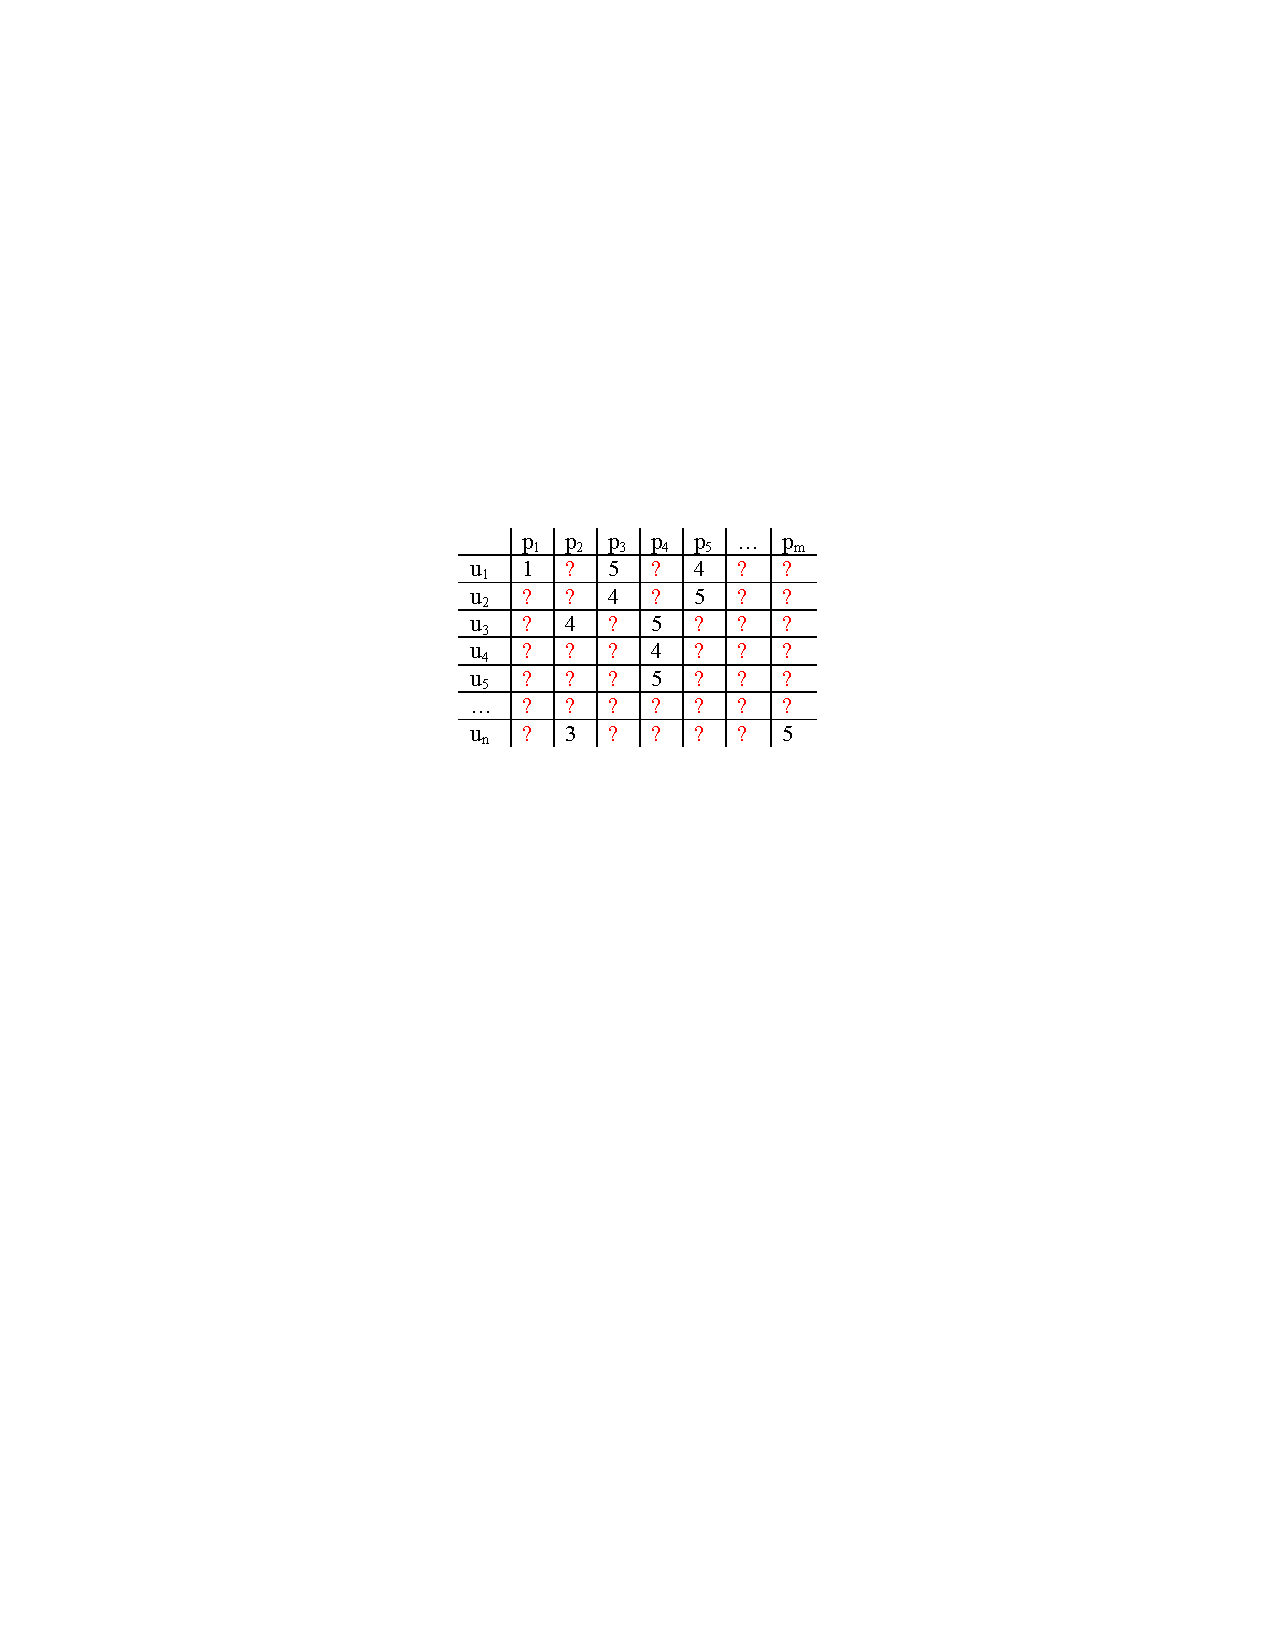
\includegraphics[width=0.45\textwidth]{Figure_1_1.pdf}
  \caption{Dấu ? là các giá trị cần tiên đoán trong ma trận đánh giá}\label{fig:figure_1_1}
\end{center}
\end{figure}

Tiếp cận CF được xem là tiếp cận thành công nhất để xây dựng các hệ thống khuyến nghị và ứng dụng rộng rãi trong lĩnh vực thương mại điện tử \cite{Su:2009:SCF, Jannach:2010:RSI}. Ý tưởng chung của tiếp cận CF là khai thác thông tin, hành vi quá khứ của người dùng dựa trên các đánh giá sẵn có từ ma trận đánh giá để tiên đoán, lượng hóa mức độ hữu ích của các đối tượng khuyến nghị mà người dùng chưa biết. Các nghiên cứu tổng quan về hệ khuyến nghị đã thực hiện khảo sát, phân loại, cũng như thực nghiệm, đánh giá các thuật toán CF. Các phương pháp CF nói chung được phân thành hai nhóm chính: (1) CF dựa trên bộ nhớ như các thuật toán tính toán tương tự, lân cận; (2) CF dựa trên mô hình như các thuật toán gom cụm, phân lớp Bayesian. Phần tiếp theo sẽ trình bày chi tiết về các nhóm thuật toán CF và các nghiên cứu liên quan. 
\subsubsection{Tiếp cận CF dựa trên bộ nhớ}
Các hệ thống CF dựa trên bộ nhớ thường dùng các kỹ thuật thống kê để tìm kiếm những người dùng, hoặc các đối tượng khuyến nghị tương tự nhau dựa trên thông tin đánh giá, hành vi quá khứ của người dùng từ ma trận đánh giá. Tiếp cận CF dựa trên bộ nhớ tìm cách ước lượng giá trị hàm hữu ích $f(u,p)$ của đối tượng khuyến nghị $p$ với người dùng $u$ dựa trên những đánh giá của những người đồng sở thích của $u$ đối với $p$ (lọc dựa trên người dùng), hoặc dựa trên những đánh giá của $u$ với các đối tượng khuyến nghị $p'$ tương tự với $p$ (lọc dựa trên đối tượng khuyến nghị). Về cơ bản, thì các thuật toán, kỹ thuật tính toán cho lọc cộng tác dựa trên người dùng và lọc dựa trên đối tượng khuyến nghị từ ma trận đánh giá là tương tự nhau. Có khác chăng là kích thước của không gian người dùng và không gian đối tượng khuyến nghị sẽ ảnh hưởng đến tốc độ tính toán khi xác định nhóm các đối tượng tương tự.

\subsubsection*{a) Lọc dựa trên người dùng}
\textbf{Định nghĩa 1.8:} \textit{Những người đồng sở thích}

Cho $U$ là không gian người dùng, gọi $S_{u}$ là tập những người đồng sở thích với $u \in U$, $S_{u} \subseteq U$. Những người đồng sở thích với $u$ là những người có hành vi quá khứ hay các đánh giá tương tự với $u$ trên cùng những đối tượng khuyến nghị từ ma trận đánh giá R \cite{Breese:1998:EAP:2074094.2074100, Su:2009:SCF, Jannach:2010:RSI}.
\\\textbf{(*) Ý tưởng chính}: với các phương pháp lọc dựa trên người dùng, hệ thống thường phải thực hiện ba bước chính: một là xác định tập những người đồng sở thích với $u$, tức $S_{u}$; hai là ước lượng giá trị hàm hữu ích $f(u,p)$ của đối tượng khuyến nghị $p$ cho người dùng $u$ bằng cách tổng hợp những đánh giá của $S_{u}$ đối với $p$; ba là thực hiện khuyến nghị dựa trên giá trị hàm hữu ích đã ước lượng được \cite{Jannach:2010:RSI, Su:2009:SCF}. Hình \ref{fig:figure_1_2} minh họa việc thực hiện khuyến nghị dùng phương pháp lọc dựa trên người dùng.
\begin{figure}[ht]
\begin{center}
\advance\leftskip-3cm
\advance\rightskip-3cm
  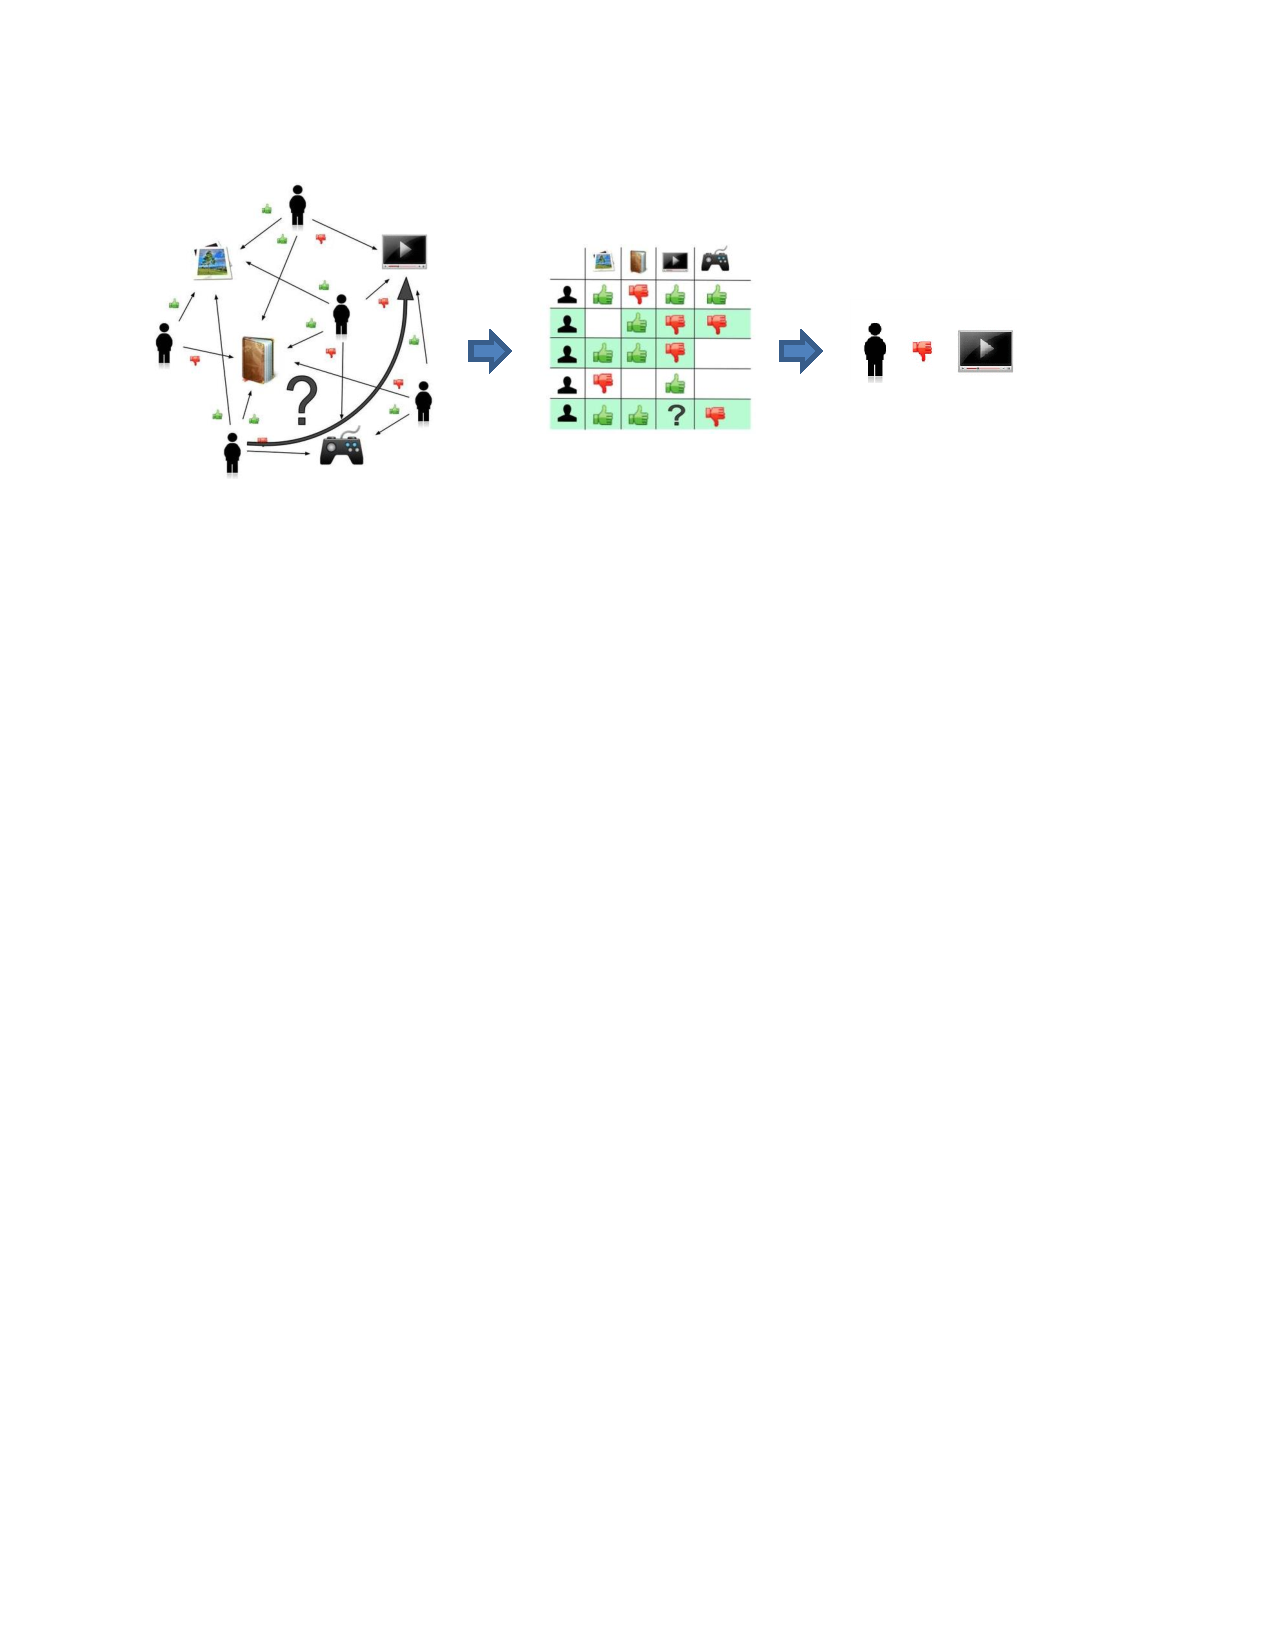
\includegraphics[width=0.95\textwidth]{Figure_1_2.pdf}
  \caption{Minh họa dùng CF để tiên đoán một người thích hay không thích xem phim.}\label{fig:figure_1_2} (Nguồn: http://en.wikipedia.org/wiki/Collaborative\_filtering)
\end{center}  
\end{figure}
\\\textbf{(**) Các bước thực hiện}: Jannach và cộng sự \cite{Jannach:2010:RSI}, Su và Khoshgoftaar \cite{Su:2009:SCF} đã khảo sát, phân tích, trình bày về các phương pháp CF khác nhau. Các bước thực hiện của phương pháp CF dựa trên người dùng có thể tóm tắt dưới dạng mã giả như sau:
\begin{algorithm}[H]
\floatname{algorithm}{Phương pháp:}	
\text{\textbf{Đầu vào}:} 
	\begin{itemize}
		\item Không gian người dùng $U = \{{u_{1}, u_{2}, ..., u_{n}}\}$, đối tượng khuyến nghị $P = \{{p_{1}, p_{2}, ..., p_{m}}\}$
		\item Ma trận đánh giá $R = \{r_{i,j\}}$,  với $i \in 1...n, j \in 1...m$ 
	\end{itemize}
	\text{\textbf{Đầu ra}:} $ \forall u \in U$, trả về Top-N$(r_{u,p})$ (tức Top-N những đối tượng khuyến nghị $p \in P$ dựa trên giá trị đánh giá tiên đoán được $r_{u,p}$)\\
	\text{--------------------------------------------------------------------------------------------------------------}
\begin{algorithmic}[1]	
\State $\forall u \in U, \forall u_{i} \in U | u_{i} \neq u,$

\text{(1) Tương tự sở thích dùng độ đo cosine:}
\begin{equation}
\displaystyle sim(u,u_{i}) = 
\frac{\overrightarrow{u} \bullet \overrightarrow{u_{i}}}{\parallel \overrightarrow{u} \parallel \ast \parallel \overrightarrow{u_{i}}\parallel} = 
\frac{\sum_{p \in P_{u,u_{i}}}^{} r_{u,p}*r_{u_{i},p}}
{\sqrt{\sum_{p \in P_{u,u_{i}} }^{}r_{u,p}^2} * \sqrt{\sum_{p \in P_{u,u_{i}} }^{}r_{u_{i},p}^2}}
\end{equation}

\text{(2) Tương tự sở thích dùng hệ số tương quan Pearson:}
\begin{equation}
\displaystyle sim(u,u_{i}) = \frac{\sum_{p \in P_{u,u_{i}}} (r_{u,p} - \overline{r}_{u})(r_{u_{i},p} - \overline{r}_{u_{i}})}
{
\sqrt{
\sum_{p \in P_{u,u_{i}}}^{}(r_{u,p} - \overline{r}_{u})^2 * 
\sum_{p \in P_{u,u_{i}}}^{}(r_{u_{i},p} - \overline{r}_{u_{i}})^2}
}
\end{equation}
{Trong đó,}
\begin{itemize}
	\item $r_{u,p}$: giá trị đánh giá của $u$ với $p$ trong ma trận đánh giá $R$.
	\item $P_{u,u_{i}} = \{p \in P | r_{u,p} \neq \oslash \: \& \: r_{u_{i},p} \neq \oslash \}$; 
	\item $\displaystyle \overline{r}_{u} = \frac{1}{|P_{u}|}\sum_{p \in P_{u}}^{}r_{u,p}$, với $P_{u} = \{p \in P | r_{u,p} \neq \oslash \}$
\end{itemize}
\State $ \forall u \in U, p \in P,$ If ($r_{u,p} \neq \oslash$ then)
\State{Begin}

\text{(1) Trung bình đánh giá}.
\begin{equation}
\displaystyle r_{u,p} = \frac{1} {|S_{u}|} \sum_{u_{i} \in S_{u }}^{}{r_{u_{i},p}}
\end{equation}
$\forall u \in U, \forall u_{i} \in U | u_{i} \neq u, S_u =  $Top-N$ (\{u_i\})$ (với $Sim(u,u_i) \geq Sim(u,u_{i+1})$)

\text{(2) Tổng hợp đánh giá có trọng số}.
\begin{equation}
\displaystyle  r_{u,p} = 1/\sum_{u_{i} \in S_{u }}|sim(u,u_{i})| * \sum_{u_{i} \in S_{u }}^{}sim(u,u_{i})*r_{u_{i},p}
\end{equation}

\text{(3) Tổng hợp dựa trên khoảng đánh giá}. 
\begin{equation}
\displaystyle  r_{u,p}  = \overline{r}_{u} + 1/\sum_{u_{i} \in S_{u }}|sim(u,u_{i})| * \sum_{u_{i} \in S_{u }}^{}sim(u,u_{i})*(r_{u_{i},p} - \overline{r}_{u_{i}})
\end{equation}
\STATE{End}
\STATE $ \forall u \in U, p \in P,$ return Top-N$(r_{u,p})$.
%\algstore{UserBasedCF}
\end{algorithmic}
\caption{CF dựa trên người dùng}
\end{algorithm}
%\begin{algorithm}[H]
%	\begin{algorithmic}[1]
%		\algrestore{UserBasedCF}	
%\end{algorithmic}
%\end{algorithm}

\subsubsection*{b) Lọc dựa trên đối tượng khuyến nghị}
Sarwar và cộng sự đã đề xuất một phương pháp CF mới, là lọc dựa trên đối tượng khuyến nghị, thay vì lọc dựa trên người dùng như các hệ thống CF truyền thống. Tương tự lọc dựa trên người dùng, lọc dựa trên đối tượng khuyến nghị cũng bao gồm 3 bước chính: một là xác định Top-N các đối tượng khuyến nghị tương tự nhất với đối tượng khuyến nghị $p$, $I_{p}$; hai là ước lượng giá trị hàm hữu ích $f(u,p)$ của đối tượng khuyến nghị $p$ cho người dùng $u$ bằng cách tổng hợp những đánh giá của $u$ cho $p \in I_{p}$; và ba là thực hiện khuyến nghị. Sarwar và cộng sự đã tiến hành thực nghiệm trên tập dữ liệu MovieLen, cho thấy các phương pháp lọc dựa trên đối tượng khuyến nghị cho kết quả tốt hơn các phương pháp lọc dựa trên người dùng \cite{Sarwar:2001:ICF}.

\subsubsection{Tiếp cận CF dựa trên mô hình}
Theo quan điểm xác suất, thì các thuật toán CF dựa trên mô hình cần tính toán xác suất mà người dùng $u$ có đánh giá $r_{u,p}$ cho một đối tượng khuyến nghị $p$, $P(r_{u,p} | u,p)$. Quá trình đó có thể xem như việc tính toán giá trị kỳ vọng cho đánh giá của người dùng $u$ với đối tượng khuyến nghị $p$ \cite{Breese:1998:EAP:2074094.2074100}. 

%Giả sử các đánh giá nhận giá trị nguyên trong khoảng từ 0 đến max. Khi đó,
%\begin{equation}
%f(u,p) = E(r_{u,i}) = \sum_{k=0}^{max}k*Pr(r(u_{x},i) = k | r(u_{x},i'), i' \in I_{u_{}} )
%\end{equation}

Khác với CF dựa trên bộ nhớ, các thuật toán CF dựa trên mô hình sẽ dùng tập các đánh giá có sẵn trong ma trận đánh giá R để học một mô hình đánh giá cho mỗi người dùng. Sau đó, mô hình học được sẽ dùng để tiên đoán các đánh giá khác. Breese và cộng dự đã khảo sát và trình bày hai cách tiếp cận CF dựa trên mô hình gom cụm và mạng Bayes \cite{Breese:1998:EAP:2074094.2074100}. Phần tiếp theo trình bày và phân tích một số nghiên cứu liên quan.

\subsubsection*{a) Các thuật toán CF gom cụm}
Một cụm bao gồm tập hợp các đối tượng dữ liệu tương tự nhau. Các đối tượng dữ liệu sẽ tương tự với các đối tượng dữ liệu khác thuộc cùng một cụm và sẽ khác biệt với các đối tượng dữ liệu trong cụm khác. Gom cụm là một kỹ thuật khá phổ biến trong lĩnh vực khai thác dữ liệu. Một số phương pháp gom cụm phổ biến có thể kế đến như: k-means \cite{citeulike:176467}, DBSCAN \cite{Ester96adensity-based}. Các nghiên cứu liên quan thông thường sẽ dùng những kỹ thuật gom cụm để phân chia dữ liệu thành những cụm, sau đó áp dụng các thuật toán CF dựa trên bộ nhớ để thực hiện tiên đoán bên trong mỗi cụm  \cite{Connor01clusteringitems, citeulike:6841553}.

Những thuật toán CF dựa trên mô hình gom cụm nói chung có khả năng mở rộng tốt hơn các thuật toán CF thông thường, vì nó đã thực hiện tiên đoán bên trong các cụm có kích thước nhỏ hơn thay vì cả không gian ma trận đánh giá và cơ sở dữ liệu quan sát. Vì độ phức tạp và chi phí tính toán gom cụm, nên việc gom cụm có thể thực hiện offline. Tuy nhiên, kết quả nghiên cứu thực nghiệm cho thấy chất lượng khuyến nghị không cao khi thực hiện gom cụm \cite{Su:2009:SCF}.

\subsubsection*{b) Các thuật toán CF dựa trên xác suất Bayes}
Tác giả Su và Khoshgoftaar đã trình bày thuật toán CF Bayes đơn giản nhất, đó là dùng xác suất Bayes ngây thơ để thực hiện tiên đoán \cite{Su:2009:SCF}. Nhãn lớp trong trường hợp này thông thường là các giá trị nguyên có thể gán cho kết quả tiên đoán (nhãn k=0, .., max). Giả sử những đặc trưng là độc lập với các lớp, khi đó xác suất mà đánh giá của $u$ cho $p$ thuộc về một lớp nào đó sẽ được tính. Lớp có xác suất cao nhất sẽ được chọn là kết quả tiên đoán. Việc tính toán xác suất, và tiên đoán được thực hiện dựa trên dữ liệu đã quan sát được.
\begin{equation} 
\displaystyle ClassLabel(u,p) = \underset{k = 0..max} {\mathrm{argmax}} \; P(class_{k})*
\displaystyle\prod\limits_{j=1}^{n} P( r_{j} \; | \; class_{k})
\end{equation}

Để làm mịn giá trị xác suất cũng như tránh trường hợp xác suất điều kiện bằng 0, các tác giả Su và Khoshgoftaar đã đề xuất dùng bộ ước lượng Laplace (Laplace Estimator) khi tính xác suất có điều kiện \cite{Su:2009:SCF}. Cụ thể như sau:
\begin{equation} \label{equation:LalaceEstimator}
P(X_{i} = x_{i} | Y = y) = \frac{\#(X_{i}=x_{i},Y=y) + 1}{\#(Y=y) + |X_{i}|}
\end{equation}
\begin{table}[ht]
\centering
    \caption{Ví dụ tiên đoán đánh giá} \label{tab:table_1_1}
    \begin{tabular}{p{1.5cm}|p{1.5cm}|p{1.5cm}|p{1.5cm}|p{1.5cm}|p{1.5cm}}
    \hline
    & $p_{1}$ & $p_{2}$ & $p_{3}$ & $p_{4}$ & $p_{5}$ \\
    \hline 
	$u_{1}$ & 4 & 1 & 5 & 5 & \textbf{?} \\
    $u_{2}$ & ? & ? & 4 & 4 & 5 \\
    $u_{3}$ & 1 & ? & 4 & 2 & 1 \\
    $u_{4}$ & ? & ? & 4 & 2 & 3 \\
    \hline
    \end{tabular}
\end{table}
\textbf{Ví dụ minh họa}: Cho ma trận đánh giá như trong bảng \ref{tab:table_1_1}. Tập các giá trị đánh giá là \{1, 2, 3, 4, 5\}. Yêu cầu đặt ra là cần tiên đoán đánh giá của $u_{1}$ với $p_{5}$. Dùng thuật toán CF Bayes đơn giản nhất và phương pháp ước lượng Laplace để tính xác suất có điều kiện như trong công thức \ref{equation:LalaceEstimator}, chúng ta có thể tính như sau:
\begin{equation} 
\begin{split}
\displaystyle ClassLabel(u_{1},p_{5}) = 
\underset{c_{k} \in \{1,2,3,4,5\}} {\mathrm{argmax}} \; P(c_{k} | u_{2}=5, u_{3}=1, u_{4}=3) \\
= \underset{c_{k} \in \{1,2,3,4,5\}} {\mathrm{argmax}} \; P(c_{k})P(u_{2} = 5 | c_{k})P(u_{3} = 1 | c_{k})P(u_{4}=3|c_{k}) \\
\end{split}
\end{equation}

Trong đó,
\begin{itemize}
\item $P(1)P(u_{2} = 5 | 1)P(u_{3} = 1 | 1)P(u_{4}=3|1) = (1/4)*(1/6)*(1/6)*(1/6) =  0.00116$
\item $P(2)P(u_{2} = 5 | 2)P(u_{3} = 1 | 2)P(u_{4}=3|2) = 0$
\item $P(3)P(u_{2} = 5 | 3)P(u_{3} = 1 | 3)P(u_{4}=3|3) = 0$
\item $P(4)P(u_{2} = 5 | 4)P(u_{3} = 1 | 4)P(u_{4}=3|4) = (1/4)*(1/6)*(2/6)*(1/6) = 0.00231$
\item $P(5)P(u_{2} = 5 | 5)P(u_{3} = 1 | 5)P(u_{4}=3|5) = (2/4)*(1/7)*(1/7)*(1/7) = 0.00146$
\end{itemize}

Như vậy,
$
\displaystyle ClassLabel(u_{1},p_{5}) = 
\underset{c_{k} \in \{1,2,3,4,5\}} {\mathrm{argmax}} \; \{0.00116, 0, 0, 0.00231, 0.00146\} = 4\\
$

\subsubsection*{c) Thừa số hóa ma trận (Matrix Factorization)}
Bên cạnh các phương pháp CF dựa trên tính toán lân cận, gom cụm và xác suất Bayes đã đề cập ở trên thì các mô hình đặc trưng tiềm ẩn (latent factor model) là một chọn lựa khác cho tiếp cận CF. Theo Koren và đồng nghiệp, các mô hình đặc trưng tiềm ẩn tìm cách biểu diễn thông tin của những người dùng và đối tượng khuyến nghị trong ma trận đánh giá thông qua 20 đến 100 đặc trưng tiềm ẩn rút trích từ các mẫu đánh giá. Những hiện thực thành công nhất của các mô hình đặc trưng tiềm ẩn là dựa trên kỹ thuật thừa số hóa ma trận (Maxtrix Factorization) \cite{Koren:2008}.

Các kỹ thuật thừa số hóa ma trận về cơ bản là dựa trên các tính toán ma trận. Thừa số hóa ma trận thực hiện việc tìm kiếm hai hay nhiều ma trận mà tích của chúng chính là ma trận ban đầu. Thừa số hóa ma trận giúp hệ thống làm việc trên không gian dữ liệu có kích thước nhỏ hơn (giảm chiều). Các nghiên cứu liên quan đã chỉ ra rằng các kỹ thuật thừa số hóa ma trận hiệu quả hơn hẳn các phương pháp lọc cộng tác truyền thống dựa trên người dùng (user-based) và dựa trên đối tượng khuyến nghị (item-based). Thừa số hóa ma trận đã góp phần giải quyết được tình trạng dữ liệu lớn, thưa trong ma trận đánh giá mà các phương pháp CF truyền thống phải đương đầu, giúp khám phá ra các đặc trưng tiềm ẩn thể hiện bản chất của những tương tác giữa người dùng và đối tượng khuyến nghị trong ma trận đánh giá.

Năm 2006, Netflix, một công ty cho thuê phim hàng đầu thế giới, đã thông báo tổ chức một cuộc thi nhằm cải tiến hệ thống khuyến nghị phim của họ. Netflix đã công bố một tập dữ liệu gồm 100 triệu đánh giá của khoảng 500.000 khách hàng với hơn 17.000 phim. Mỗi đánh giá sẽ nhận các giá trị từ 1 đến 5. Công ty kêu gọi và thách thức cộng đồng khoa học máy tính phát triển các phương pháp máy học, khai thác dữ liệu làm thế nào để cải tiến độ chính xác khuyến nghị của hệ thống khuyến nghị phim Netflix \cite{bennett2007netflix}. Năm 2008, Koren và cộng sự đã công bố phương pháp thừa số hóa ma trận cho CF và đã thắng giải thưởng Netflix trị giá 1 triệu USD \cite{Koren:2008}. Từ đó đến nay, các kỹ thuật thừa số hóa ma trận tiếp tục được phát triển và trở thành một trong những tiếp cận nổi trội cho hệ khuyến nghị nói chung và tiếp cận CF nói riêng. 

Những mô hình thừa số hóa ma trận tìm cách ánh xạ không gian người dùng và đối tượng khuyến nghị (ma trận đánh giá) vào một không gian đặc trưng tiềm ẩn với số chiều là $k$. Ở đó, những tương tác giữa người dùng và đối tượng khuyến nghị trong ma trận đánh giá sẽ được mô hình như các tích vô hướng trong không gian đó. Mỗi đối tượng khuyến nghị $p \in P$ tương ứng với một vectơ $\overrightarrow{a_{p}}\in \mathbb{R}^k$. Mỗi người dùng $u \in U$ tương ứng với một vectơ $\overrightarrow{b_u} \in \mathbb{R}^k$. Với một đối tượng $p \in P$, những thành phần của $\overrightarrow{a_{p}}$ đo lường mức độ mà đối tượng $p$ có được ở những đặc trưng đó. Đối với một người dùng $u \in U$, những thành thành của $\overrightarrow{b_u}$ đo lường mức độ quan tâm mà $u$ thể hiện đối với các đối tượng khuyến nghị $p \in P$ có giá trị cao ở những đặc trưng tiềm ẩn tương ứng đó. Tích vô hướng $\overrightarrow{a_{p}}.\overrightarrow{b_u}$ thể hiện tương tác giữa người dùng $u$ và đối tượng $p$ (quan tâm của $u$ trên các đặc trưng của $p$). Giá trị tính được trong không gian đặc trưng tiềm ẩn sẽ xấp xỉ với giá trị đánh giá của $u$ đối với $p$ ($r(u,p)$). Do đó, giá trị đánh giá của $u$ với $p$ có thể được ước lượng, tiên đoán như sau:

\begin{equation}\label{RatingPredictionMF}
\hat{r}(u,p) = \overrightarrow{a_{p}}.\overrightarrow{b_u}
\end{equation}

Trong đó,
\begin{itemize}
	\item $\hat{r}(u,p)$: giá trị đánh giá thể hiện quan tâm của $u$ với $p$ tiên đoán được trong không gian $\mathbb{R}^k$. 
	\item $\overrightarrow{a_{p}}$: vectơ biểu diễn đối tượng $p$ trong không gian đặc trưng tiềm ẩn $\mathbb{R}^k$.
	\item $\overrightarrow{b_{u}}$: vectơ biểu diễn người dùng $u$ trong không gian đặc trưng tiềm ẩn $\mathbb{R}^k$.
\end{itemize}

Vấn đề đặt ra là làm thế nào để ánh xạ $p \in P, u \in U$ thành những vectơ đặc trưng tiềm ẩn $\overrightarrow{a_{p}},\overrightarrow{b_{u}} \in \mathbb{R}^k$. Khi ánh xạ này được xác định, hệ thống có thể ước lượng giá trị đánh giá của bất kỳ $u \in U$ với $p \in P$ dùng công thức \ref{RatingPredictionMF}. Một mô hình như thế liên quan đến phương pháp phân tích giá trị đặc biệt (Singular Value Decomposition), gọi tắt là SVD, một kỹ thuật dùng để xác định các đặc trưng ngữ nghĩa tiềm ẩn trong lĩnh vực truy vấn thông tin. Để áp dụng SVD cho lọc cộng tác thì ma trận đánh giá cần phải được thừa số hóa. Điều này sẽ gặp khó khăn vì ma trận đánh giá thưa (nhiều giá trị đánh giá chưa xác định). Thông thường, SVD sẽ không định nghĩa được khi thông tin trong ma trận không đầy đủ. Hơn nữa, dựa trên một số ít phần tử trong ma trận để tính toán thì dễ dẫn đến vấn đề quá khớp. Dẫn đến việc tiên đoán không chính xác.

Các nghiên cứu phổ biến thường dùng một số kỹ thuật tính toán để khởi tạo và làm đầy những chỗ thiếu thông tin trong ma trận đánh giá. Tuy nhiên, việc tính toán đó sẽ tốn nhiều chi phí khi kích thước dữ liệu gia tăng. Thêm vào, việc tính toán không chính xác có thể dẫn đến những sai lệch đáng kể trong dữ liệu. Do đó, một số nghiên cứu khác đã đề xuất việc mô hình hóa trực tiếp chỉ dựa trên những đánh giá quan sát được.

Nói chung, để học và xác định những vectơ đặc trưng tiềm ẩn $\overrightarrow{a_{p}}, \overrightarrow{b_{u}}$, hệ thống cần phải tối tiểu hóa lỗi bình phương dựa trên các đánh giá đã biết như sau:

\begin{equation}\label{SquaredError_MF}
min \sum\limits_{(u,p) \in K}^{}(r(u,p) - \hat{r}(u,p))^2 + \lambda(||\overrightarrow{a_{p}}||^2 + ||\overrightarrow{b_{u}}||^2)
\end{equation}

Trong đó,
\begin{itemize}
\item $K$: tập các cặp $(u,p)$ mà giá trị $r(u,p)$ được biết trước (dữ liệu huấn luyện).
\item $\lambda$: hằng số kiểm soát vấn đề quá khớp khi học dựa trên dữ liệu quan sát, được xác định thông qua việc cross-validation (Thực nghiệm có thể chọn $\lambda$ là 0.1, 0.2, ..., 1).
\end{itemize}

Hệ thống sẽ học một mô hình bằng cách cực tiểu hóa lỗi bình phương theo công thức \ref{SquaredError_MF} để xấp xỉ tốt nhất với những đánh giá đã quan sát được.
\subsubsection*{Phương pháp phân tích giá trị đặc biệt (Singular Value Decomposition)} 
SVD cho phép phân tích một ma trận $R_{mn}$ thành tích của 3 ma trận đó là: một ma trận trực giao $U$, một ma trận đường chéo $S$ và một ma trận chuyển vị của ma trận trực giao $V$ \cite{kb2005}.
%Hình \ref{fig:figure_1_10} minh họa phương pháp SVD, phân rã ma trận $X_{mn}$ thành 3 ma trận $U_{mn}, S_{nn}$ và $V_{nn}$.

%\begin{figure}[ht]
%	\begin{center}
%		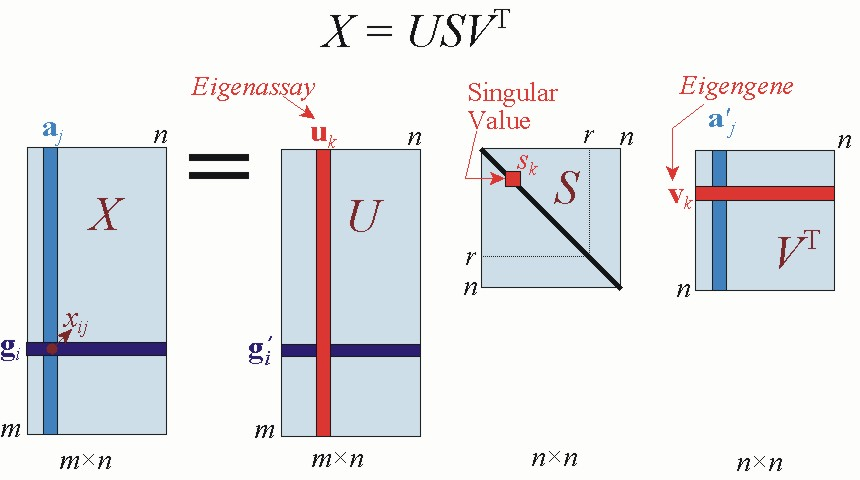
\includegraphics[width=0.70\textwidth]{Figure_1_10.jpg}
%		\caption{Minh họa phương pháp SVD}\label{fig:figure_1_10}
%		(Nguồn hình vẽ: http://public.lanl.gov/mewall/kluwer2002.html)
%	\end{center}
%\end{figure}

\begin{equation}
R_{mn} = U_{mm}S_{mn}V_{nn}^T
\end{equation}

Trong đó,
\begin{itemize}
	\item $U^TU = I; V^TV = I$ ($I$: ma trận đơn vị)
	\item Cột của ma trận trực giao $U$ là các vectơ riêng trực chuẩn của $RR^T$
	\item Cột của ma trận trực giao $V$ là các vectơ riêng trực chuẩn của $R^TR$
	\item $S$ là ma trận đường chéo, căn bậc 2 của những giá trị riêng từ U hay V theo thứ tự giảm dần.
\end{itemize}

Để xác định các đặc trưng tiềm ẩn (giảm chiều) khi thực nghiệm, SVD chọn số đặc trưng tiềm ẩn $k \leq min(m, n)$. Khi đó, phương pháp SVD sẽ học để xác định 3 ma trận $U, S, V$ mà tích của chúng là $\hat{R_{mn}}$ (ma trận xấp xỉ tốt nhất với ma trận ban đầu $R_{mn}$) bằng cách cực tiểu lỗi bình phương (công thức \ref{SquaredError_MF}). 

\begin{equation}
\hat{R_{mn}} = U_{mm}S_{mk}V_{kn}^T
\end{equation}

%Dựa trên lý thuyết đại số tuyến tính, việc phân rã một ma trận $R$ dùng phương SVD có thể được minh họa thông qua ví dụ tiếp sau.\\
%\textbf{Ví dụ minh họa} (Nguồn \cite{kb2005}): Áp dụng SVD để phân tích một ma trận $R$:
%\begin{center}
%$
%R =
%\begin{bmatrix}
%	3 & 1 & 1 \\
%	-1 & 3 & 1 \\
%\end{bmatrix}
%$
%\end{center}
%
%Dựa trên lý thuyết đại số tuyến tính, việc phân tích ma trận $R$ có thể thực hiện như sau:
%
%\begin{itemize}
%	\item Để tìm ma trận $U, S, V$, đầu tiên ta cần xác định $RR^T$.
%\end{itemize}
%
%Ta có, 
%\begin{center}
%$RR^T
%= \begin{bmatrix}
%3 & 1 & 1 \\
%-1 & 3 & 1 \\
%\end{bmatrix}
%\begin{bmatrix}
%3 & -1 \\
%1 & 3 \\
%1 & 1 \\
%\end{bmatrix}
%= 
%\begin{bmatrix}
%11 & 1 \\
%1 & 11 \\
%\end{bmatrix}
%$
%\end{center}
%
%\begin{itemize}
%\item Tiếp theo, ta cần xác định trị riêng và vectơ riêng của $RR^T$. Gọi $\lambda, \overrightarrow{v}$ lần lượt là trị riêng và vectơ riêng của $RR^T$. Tức là $RR^T\overrightarrow{v} = \lambda\overrightarrow{v}$. Cụ thể là,
%\end{itemize}
%
%\begin{center}
%	$
%\begin{bmatrix}
%	11 & 1 \\
%	1 & 11 \\
%\end{bmatrix}
%\begin{bmatrix}
%x_{1} \\
%x_{2} \\
%\end{bmatrix}
%=
%\lambda
%\begin{bmatrix}
%x_{1} \\
%x_{2} \\
%\end{bmatrix}
%$
%($x_1, x_2$ là 2 thành phần của $\overrightarrow{v}$)
%\end{center}
% 
%Như vậy, ta cần giải hệ phương trình sau:
%\begin{center}
%	$(11 - \lambda)x_{1} + x_{2} = 0$ \\
%	$x_{1} + (11 - \lambda)x_{2} = 0$
%\end{center}
%
%Để tính $\lambda$, ta cần gán định thức của ma trận hệ số bằng 0. Tức
%\begin{center}
%$
%\begin{vmatrix}
%	(11 - \lambda) & 1 \\
%	1 & (11 - \lambda) \\
%\end{vmatrix}
%= 0 
%$
%\end{center}
%\begin{center}
%$(11 - \lambda)^2 - 1 = 0 $
%\end{center}
%\begin{center}
%$\lambda = 10, \lambda = 12$
%\end{center}
%
%Thế giá trị riêng $\lambda$ vào hệ phương trình ban đầu để tìm các vectơ riêng $\overrightarrow{v}$.\\
%Với  $\lambda = 10$, thì $x_1 = -x_2$. Có vô số vector tiêng thỏa điều kiện. Để đơn giản, ta chọn $x_1 = 1$, suy ra  $x_2 = -1$ \\
%Với  $\lambda = 12$, thì  $x_1 = x_2$. Tương tự, ta chọn $x_1 = 1$, suy ra  $x_2 = 1$ \\
%
%Các vectơ riêng sẽ là những vectơ cột trong một ma trận được sắp xếp theo thứ tự tương ứng giảm dần của giá trị riêng. Nói cách khác, vectơ riêng của trị riêng lớn nhất là cột 1, cột 2 là vectơ riêng của trị riêng lớn thứ 2 và cột cuối cùng là vectơ riêng của trị riêng nhỏ nhất. Với ví dụ này, vectơ riêng của $\lambda = 12$ cột 1; Cột 2 là vectơ riêng của trị riêng $\lambda = 10$.
%
%\begin{center}
%$
%\begin{bmatrix}
%1 & 1 \\
%1 & -1 \\
%\end{bmatrix}
%$
%\end{center}
%
%\begin{itemize}
%	\item Chuyển ma trận này thành ma trận trực giao theo phương pháp Gram-Schmidt \cite{kb2005}, ta được ma trận $U$.
%\end{itemize}
%
%\begin{center}
%	$
%	U =
%	\begin{bmatrix}
%	\frac{1}{\sqrt{2}} & \frac{1}{\sqrt{2}} \\
%	\frac{1}{\sqrt{2}} & \frac{-1}{\sqrt{2}} \\
%	\end{bmatrix}
%	$
%\end{center}
%
%\begin{itemize}
%	\item Tương tự, để tìm $V$, ta cần tìm trị riêng và vectơ riêng của $R^TR$.
%\end{itemize}
%
%\begin{center}
%$
%\begin{bmatrix}
%3 & -1 \\
%1 & 3 \\
%1 & 1 \\
%\end{bmatrix}
%\begin{bmatrix}
%3 & 1 & 1 \\
%-1 & 3 & 1 \\
%\end{bmatrix}
%= 
%\begin{bmatrix}
%10 & 0 & 2 \\
%0 & 10 & 4 \\
%2 & 4 & 2 \\
%\end{bmatrix}
%$
%\end{center}
%
%Gọi $\lambda, \overrightarrow{v}$ lần lượt là trị riêng và vectơ riêng của $R^TR$. Tức là $R^TR\overrightarrow{v} = \lambda\overrightarrow{v}$. Tương tự quá trình tìm trị riêng và vectơ riêng cho $U$, $R^TR$ có các giá trị riêng và vectơ riêng lần lượt là:
%
%\begin{center}
%$\lambda = 12, \overrightarrow{v_1} = [1,2,1]$ \\
%$\lambda = 10, \overrightarrow{v_2} = [2,-1,0]$ \\
%$\lambda = 0, \overrightarrow{v_3} = [1,2,-5]$ \\
%\end{center}
%
%Sắp xếp các vec tơ riêng này như những vectơ cột, ta được ma trận sau:
%\begin{center}
%$
%\begin{bmatrix}
%	1 & 2 & 1 \\
%	2 & -1 & 2 \\
%	1 & 0 & -5 \\
%\end{bmatrix}
%$
%\end{center}
%
%\begin{itemize}
%	\item Tương tự việc tìm $U$, chuyển ma trận này thành ma trận trực giao theo phương pháp Gram-Schmidt ta được ma trận $V$.
%\end{itemize}
%
%\begin{center}
%$
%V =
%\begin{bmatrix}
%\frac{1}{\sqrt{6}} & \frac{2}{\sqrt{5}} & \frac{1}{\sqrt{30}}\\
%\frac{2}{\sqrt{6}} & \frac{-1}{\sqrt{5}} & \frac{2}{\sqrt{30}}\\
%\frac{1}{\sqrt{6}} & 0 & \frac{-5}{\sqrt{30}}\\
%\end{bmatrix}
%$
%\end{center}
%
%\begin{itemize}
%	\item Để tìm S, phương pháp SVD lấy căn bậc 2 của những giá trị riêng khác không và đặt trên đường chéo. Giá trị lớn nhất đặt tại vị trí $S_{11}$, giá trị lớn thứ 2 đặt tại $S_{22}$ và cuối cùng là giá trị nhỏ nhất đặt tại $S_{mm}$. Các giá trị riêng khác không của $U$ và $V$ thì luôn giống nhau, vì vậy ta có thể chọn những giá trị này từ $U$ hoặc $V$. Một vectơ cột có các thành phần 0 được thêm vào $S$ để đảm bảo số chiều phù hợp khi nhân với 2 ma trận $U$, $V$. Đường chéo của $S$ là các giá trị đặc biệt của $R$, cột của $U$ được gọi là những vectơ đặc biệt bên trái, cột của $V$ được gọi là các vectơ đặc biệt bên phải.
%\end{itemize}
%
%\begin{center}
%$
%S =
%\begin{bmatrix}
%\sqrt{12} & 0 & 0 \\
%0 & \sqrt{10} & 0 \\
%\end{bmatrix}
%$
%\end{center}
%
%Như vậy $R$ có thể phân tích thành $U, S, V$ như sau:
%
%\begin{center}	
%$
%R_{mn} = U_{mm}S_{mn}V^T_{nn} = 
%\begin{bmatrix}
%\frac{1}{\sqrt{2}} & \frac{1}{\sqrt{2}} \\
%\frac{1}{\sqrt{2}} & \frac{-1}{\sqrt{2}} \\
%\end{bmatrix}
%\begin{bmatrix}
%\sqrt{12} & 0 & 0 \\
%0 & \sqrt{10} & 0 \\
%\end{bmatrix}
%\begin{bmatrix}
%\frac{1}{\sqrt{6}} & \frac{2}{\sqrt{6}} & \frac{1}{\sqrt{6}} \\
%\frac{2}{\sqrt{5}} & \frac{-1}{\sqrt{5}} & 0 \\
%\frac{1}{\sqrt{30}} & \frac{2}{\sqrt{30}} & \frac{-5}{\sqrt{30}} \\
%\end{bmatrix}
%= ... =
%\begin{bmatrix}
%3 & 1 & 1 \\
%-1 & 3 & 1 \\
%\end{bmatrix}
%$
%\end{center}

\subsubsection{Ưu điểm và hạn chế của tiếp cận CF}
Khác với tiếp cận nội dung, các hệ thống CF không bị các hạn chế về mặt phân tích nội dung cho các đối tượng khuyến nghị có nội dung dạng văn bản. Những hệ thống CF dùng thông tin từ ma trận đánh giá quan sát được của những người dùng khác. Vì vậy, các hệ thống CF có thể áp dụng cho nhiều dạng đối tượng, nhiều kiểu nội dung khác nhau, ngay cả với các đối tượng khuyến nghị không tương tự với các đối tượng khuyến nghị quan sát trong quá khứ. Theo các tác giả Su và Khoshgoftaar, tiếp cận CF được xem là một trong những cách tiếp cận thành công nhất để thiết kế các thuật toán và xây dựng các hệ khuyến nghị \cite{Su:2009:SCF}. Tuy nhiên, theo nghiên cứu tổng quan của các tác giả Adomavicius và Tuzhilin \cite{Adomavicius:2005:TNG:1070611.1070751}, tác giả Bobadilla và cộng sự \cite{Bobadilla2013109}, thì tiếp cận CF truyền thống cũng có một số hạn chế như sau: 
\begin{itemize}
\item \textbf{Ma trận thưa}: Đầu vào của các hệ thống CF là mà trận đánh giá. Trên thực tế thì không gian người dùng và đối tượng khuyến nghị là rất lớn. Trong khi đó số đánh giá của người dùng với các đối tượng khuyến nghị thực chất không nhiều. Nói chung, số lượng đánh giá quan sát được là rất nhỏ so với số lượng đánh giá cần phải tiên đoán. Điều đó ảnh hưởng đến độ chính xác tiên đoán, cũng như chất lượng khuyến nghị. Chẳng hạn, trong hệ thống khuyến nghị nhà hàng, có rất nhiều nhà hàng mới chỉ được đánh giá bởi một số rất ít người dùng. Như thế, cho dù nó có chất lượng và được đánh giá rất cao bởi một ít người dùng thì nó vẫn hiếm khi được khuyến nghị cho người dùng khác. Điều đó dẫn đến hệ thống khuyến nghị "nghèo nàn".
\item \textbf{Người dùng mới} (khởi động lạnh): Tương tự như tiếp cận dựa trên nội dung. Hệ thống CF cần phân tích hay học từ ma trận đánh giá để biết được sở thích của người dùng. Đối với người chưa có hoặc rất ít thông tin cá nhân cũng như thông tin đánh giá của họ, thì hệ thống không thể biết được sở thích của người dùng. Do đó không thể có những tiên đoán, khuyến nghị hữu ích.
\item \textbf{Đối tượng khuyến nghị mới} (khởi động lạnh): Các đối tượng khuyến nghị mới được thêm vào hệ thống một cách thường xuyên. Các hệ thống CF dựa trên sở thích người dùng để thực hiện khuyến nghị, do đó nếu những đối tượng mới chưa được ai đánh giá thì nó không thể được khuyến nghị, mặc dù có thể nó rất tương tự với một số đối tượng khuyến nghị nào đã có, hoặc rất tiềm năng với người dùng. 
\end{itemize}

Những hạn chế của tiếp cận nội dung cũng như tiếp cận CF truyền thống có thể giải quyết bằng cách kết hợp hai hay nhiều phương pháp khác nhau (tiếp cận lai) để phát triển các phương pháp khuyến nghị mới. Phần tiếp theo sẽ trình bày một số phương pháp lai phổ biến, cũng như các nghiên cứu, ứng dụng liên quan. 

\subsection{Tiếp cận lai (Hybrid Approach)}
Những phương pháp khác nhau đều có những điểm mạnh, cũng như điểm yếu của nó (bảng \ref{tab:table_1_2}). Để tận dụng những điểm mạnh và hạn chế điểm yếu của những tiếp cận khác nhau, nhiều nghiên cứu đã tập trung phát triển các hệ khuyến nghị dựa trên việc kết hợp các tiếp cận khác nhau, được gọi là tiếp cận lai (Hybrid Approach) hay hệ khuyến nghị lai (Hybrid Recommender System). Robin Burke đã khảo sát các phương pháp lai cho hệ khuyến nghị và trình báy tóm tắt 7 nhóm phương pháp tiếp cận lai khác nhau \cite{Robin:2002:HybridRS_Survey}. Phần tiếp theo sẽ trình bày tóm tắt 7 nhóm phương pháp lai này, các nghiên cứu liên quan cũng như điểm mạnh, yếu của mỗi nhóm phương pháp.

\subsubsection{Lai có trọng số (Weighted Hybrid)}
Mỗi phương pháp khuyến nghị phải đi tìm và xác định giá trị hàm hữu ích $f(u,p)$ của đối tượng $p \in P$ với người dùng $u \in U$. Tiếp cận lai có trọng số (Weighted Hybrid) tính toán giá trị của hàm hữu ích $f_{hybrid}(u,p)$ dựa trên kết quả của tất cả các $f(u,p)$ của các phương pháp khuyến nghị khác tồn tại trong hệ thống. Thông thường, hình thức lai có trọng số đơn giản nhất là kết hợp tuyến tính các giá trị hữu ích tính được từ các phương pháp khác nhau trong hệ thống. 

Tác giả Claypool và cộng sự đã lần đầu áp dụng kết hợp tuyến tính cho hệ thống lọc tin tức trực tuyến. Họ đã khởi tạo trọng số ngang nhau cho phương pháp CB và CF để tính toán giá trị hữu ích cho tin tức khuyến nghị. Sau đó, hệ thống sẽ dần hiệu chỉnh trọng số khi nhận được những đánh giá phản hồi từ người dùng \cite{Claypool:99:HybridRecSys}. Trong một nghiên cứu khác, tác giả Pazzani đã đề xuất phương pháp lai có trọng số bằng cách kết hợp tuyến tính kết quả tiên đoán (giá trị hữu ích) của 5 phương pháp khác nhau là lọc cộng tác dựa trên người dùng, lọc cộng tác dựa trên đối tượng, lọc nội dung, lọc dựa trên thông tin cá nhân (demographic filtering), lọc cộng tác kết hợp nội dung (Collaboration via Content). Giá trị hữu ích sau cùng là tổng giá trị hữu ích của 5 phương pháp khác nhau (các giá trị hữu ích từ 1 đến 5). Pazzani đã tiến hành thực nghiệm trên tập dữ liệu liên quan đến đánh giá của người dùng là sinh viên đối với các nhà hàng ở quận Cam, USA. Kết quả thực nghiệm của họ cho thấy việc kết hợp tuyến tính 5 phương pháp cho kết quả tốt hơn khi thiếu đi sự kết hợp của một phương pháp trong số đó \cite{Pazzani:1999:FCC}.

\begin{itemize}
	\item \textbf{Ưu điểm}: Tất cả khả năng, phương pháp khác nhau của hệ thống được tham gia vào quá trình khuyến nghị một cách minh bạch, tự nhiên, dễ dàng thực hiện, dễ dàng hiệu chỉnh.
\end{itemize}

\begin{itemize}
	\item \textbf{Hạn chế}: Việc ước lượng trọng số lớn hay nhỏ cho phù hợp với những phương pháp khác nhau.
\end{itemize}

\subsubsection{Lai chuyển đổi (Switching Hybrid)}
Các hệ thống khuyến nghị thuộc nhóm lai chuyển đổi (Switching Hybrid) sử dụng một số điều kiện để chuyển đổi qua lại giữa các phương pháp khuyến nghị khác nhau. Billsus và Pazzani đã giới thiệu hệ thống DailyLearner, một nghiên cứu về hệ thống dịch vụ tin tức thích nghi công bố trên mạng từ 05/1999 đến 06/2000, là một hệ thống sử dụng phương pháp lai chuyển đổi giữa tiếp cận nội dung và lọc cộng tác \cite{Billsus:2000:UMA:598285.598352}. Các tác giả áp dụng phương pháp lọc nội dung trước. Sau đó, những trường hợp mà tiếp cận nội dung không thể thực hiện khuyến nghị (giá trị hữu ích thấp) thì tiếp cận lọc cộng tác sẽ được áp dụng.
%Các tác giả đã đề xuất việc học mô hình sở thích đọc tin cho mỗi người dùng dựa trên phân tích nội dung tin tức mà người dùng quan tâm một cách rõ ràng (thông qua đánh giá) hay tiềm ẩn (thông qua hành vì đọc tin) : một mô hình sở thích ngắn hạn; một mô hình sở thích dài hạn. Mô hình sở thích ngắn hạn giúp người dùng tiếp tục theo dõi những tin tức liên quan đến một sự kiện nào đó mà họ quan tâm. Mô hình sở thích dài hạn giúp mô hình hóa sở thích, các chủ đề mà người dùng quan tâm nói chung trong một thời gian dài. Để tiên đoán mức độ hữu ích của một tin tức mới đối với người dùng, đầu tiên hệ thống dùng mô hình sở thích ngắn hạn. Nếu mô hình ngắn hạn thất bại khi phân loại tin tức, thì mô hình dài hạn sẽ được áp dụng. Nếu mô hình sở thích dài hạn cũng thất bại thì một giá trị hữu ích mặc định sẽ được gán. Vì vậy những tin tức không được phân loại 

Lọc cộng tác trong phương pháp lai chuyển đổi giúp hệ thống có thể khuyến nghị được các đối tượng có nội dung, ngữ nghĩa khác với các đối tượng đã được đánh giá cao. Nói cách khác, một đối tượng có thể không được khuyến nghị với tiếp cận nội dung, nhưng sau khi áp dụng lọc cộng tác thì đối tượng đó có thể được ưu tiên khuyến nghị.

\begin{itemize}
	\item \textbf{Ưu điểm}: Tiếp cận này rất "nhạy" với các điểm mạnh và yếu của các phương pháp khác nhau.
\end{itemize}
\begin{itemize}
	\item \textbf{Hạn chế}: Tuy "nhạy" với điểm mạnh và yếu của các phương pháp khác nhau, nhưng lai chuyển đổi yêu cầu cần phải xác định điều kiện để chuyển đổi giữa các phương pháp. Điều này làm cho quá trình khuyến nghị trở nên phức tạp hơn.
\end{itemize}

\subsubsection{Lai trộn (Mixed Hybrid)}
Tiếp cận lai trộn (mixed hybrid) thực hiện các phương pháp khuyến nghị khác nhau một cách độc lập và kết hợp kết quả từ các phương pháp này thành danh sách sau cùng đề xuất cùng lúc đến người dùng. Tiếp cận lai trộn tránh được vấn đề đối tượng khuyến nghị mới (một trường hợp của khởi động lạnh). Lọc dựa trên nội dung trong tiếp cận lai trộn giúp đề xuất các đối tượng khuyến nghị mới (chưa hoặc có rất ít đánh giá) trong danh sách sau cùng dựa trên những mô tả nội dung đối tượng này trong khi phương pháp lọc cộng tác không thể thực hiện được. Bù lại, lọc cộng tác trong lai trộn giúp đề xuất các đối tượng khuyến nghị tiềm năng nhưng không tương tự về nội dung.

Các tác giả Smyth và Cotter dùng tiếp cận lai trộn để phát triển một hệ thống khuyến nghị chương trình truyền hình phù hợp với sở thích cá nhân của người dùng, hệ thống PTV \cite{Smyth:2000:PTL}. Với PTV, những người dùng đăng ký vào hệ thống sẽ nhận được các khuyến nghị chương trình truyền hình mỗi ngày thông qua Internet. PVT xây dựng hồ sơ người dùng bằng cách cho người dùng tự cập nhật thông tin sở thích. Bên cạnh đó, hệ thống cũng ghi nhân đánh giá phản hồi của người dùng thông qua kết quả khuyến nghị. Kết quả khuyến nghị được tập hợp, trộn từ kết quả của hai phương pháp lọc nội dung và lọc cộng tác. Chất lượng, độ chính xác khuyến nghị của hệ thống PTV được đánh giá thông qua việc khảo sát ý kiến người dùng. Bênh cạnh đó, Burke cũng đã khảo sát một số hệ thống, nghiên cứu khác có sử dụng tiếp cận lai trộn như: ProfBuilder (Wasfi, 1999), PickAFlick (Burke và đồng nghiệp 1997, 2000) \cite{Robin:2002:HybridRS_Survey}. Nhìn chung, tiếp cận này có những ưu điểm hạn chế như sau:
\begin{itemize}
	\item \textbf{Ưu điểm}: Giúp đề xuất các đối tượng khuyến nghị tiềm năng mà bản thân một phương pháp riêng biệt không xác định được. Trộn lọc nội dung và lọc cộng tác giúp giải quyết được vấn đề khởi động lạnh (đối tượng khuyến nghị mới) và có thể đa dạng hóa khuyến nghị (đối tượng không tương tự về nội dung).
\end{itemize}
\begin{itemize}
	\item \textbf{Hạn chế}: Tiếp cận này nhằm tận dụng nhiều đề xuất từ nhiều phương pháp khác nhau. Vì vậy, hệ thống cần cơ chế xử lý, lọc các đề xuất đụng độ, trùng lắp từ các phương pháp khác nhau. Ở đây, nếu trộn hai phương pháp lọc nội dung và lọc cộng tác thì vẫn chưa giải quyết được vấn đề người dùng mới (một trường hợp của khởi động lạnh).
\end{itemize}

\subsubsection{Lai kết hợp đặc trưng (Feature Combination Hybrid)}
Lai kết hợp đặc trưng là tiếp cận phát triển phương pháp khuyến nghị bằng cách sử dụng kết hợp thông tin đánh giá của người dùng với nội dung của đối tượng khuyến nghị. Tác giả Basu và đồng nghiệp đã đề xuất tiếp cận học luật dựa trên việc kết hợp đặc trưng để thực hiện khuyến nghị \cite{Basu98recommendationas}. Họ đã thử nghiệm trên tập dữ liệu hơn 45.000 phim và hơn 250 người dùng. Mỗi cặp (người dùng, phim) được mã hóa thành tập các đặc trưng bao gồm đặc trưng cộng tác (rút từ ma trận đánh giá) và các đặc trưng nội dung mô tả phim. Kết quả thực nghiệm của họ cho thấy: việc sử dụng tất cả đặc trưng về nội dung cải tiến độ đo bao phủ (Recall), nhưng không cải tiến độ chính xác (Precision); việc kết hợp đặc trưng đã cải tiến đáng kể cả độ chính xác và độ bao phủ so với không kết hợp đặc trưng.

\begin{itemize}
	\item \textbf{Ưu điểm}: Lai kết hợp đặc trưng cho phép hệ thống xem xét dữ liệu cộng tác, nhưng không chỉ phụ thuộc duy nhất vào dữ liệu cộng tác trong ma trận đánh giá. Ngược lại, hệ thống cũng có được thông tin về sự tương tự vốn có giữa các đối tượng khuyến nghị (dựa trên đặc trưng nội dung) mà không bị ảnh hưởng bởi dữ liệu cộng tác.
\end{itemize}
\begin{itemize}
	\item \textbf{Hạn chế}: Khó khăn trong việc xác định các đặc trưng cộng tác và đặc trưng nội dung phù hợp.
\end{itemize}

\subsubsection{Lai theo đợt (Cascade Hybrid)}
Lai theo đợt (cascade hybrid) là tiếp cận mà các phương pháp khuyến nghị khác nhau được lần lượt áp dụng theo một thứ tự ưu tiên được xác định trước tùy vào mỗi ứng dụng cụ thể. Phương pháp khuyến nghị thứ nhất sinh ra một danh sách xếp hạng các ứng viên (danh sách thô). Tiếp đó, những phương pháp khác với độ ưu tiên thấp hơn sẽ được áp dụng để lọc lại danh sách thô này. Lai theo đợt giúp phương pháp thứ hai tránh những đối tượng có thể không bao giờ cần khuyến nghị vì những đối tượng này đã được lọc qua phương pháp thứ nhất. Đồng thời, các đối tượng được ưu tiên chọn với phương pháp thứ nhất sẽ được tinh lọc, chứ không bị loại bỏ thông qua phương pháp thứ hai. 

Entree\footnote{http://infolab.ils.nwu.edu/entree/} là một hệ thống khuyến nghị nhà hàng dựa trên tri thức. Entree dùng kỹ thuật suy luận dựa trên trường hợp (case-based reasoning) để chọn và xếp hạng những nhà hàng hỗ trợ những người tham gia một hội nghị ở Chicago năm 1996. EntreeC là một cải tiến của Entree. EntreeC áp dụng tiếp cận lai theo đợt bằng cách bổ sung thêm phương pháp lọc cộng tác để thực hiện việc tinh lọc ở đợt thứ 2 so với dợt lọc đầu tiên dựa trên tri thức của Entree \cite{Robin:2002:HybridRS_Survey}. 

\begin{itemize}
	\item \textbf{Ưu điểm}: So với tiếp cận lai có trọng số (Weighted Hybrid) và một số tiếp cận lai khác thì việc lọc lại danh sách thô làm cho tiếp cận này hiệu quả hơn bởi vì các phương pháp tiếp theo chỉ thực hiện lọc trên một không gian nhỏ hơn (danh sách thô), thay vì trên cả không gian tất cả các đối tượng khuyến nghị.
\end{itemize}
\begin{itemize}
	\item \textbf{Hạn chế}: Khó khăn trong việc xác định độ ưu tiên giữa các phương pháp khác nhau cho mỗi ứng dụng cụ thể.
\end{itemize}

\subsubsection{Lai tăng cường đặc trưng (Feature Augmentation Hybrid)}
Với tiếp cận lai tăng cường đặc trưng, phương pháp đầu sẽ học một mô hình để sinh ra đặc trưng tăng cường cho đầu vào phương pháp tiếp theo. Tác giả Mooney và Roy đã giới thiệu một hệ thống thử nghiệm LIBRA (Learning Intelligent Book Recommending Agent) dùng cơ sở dữ liệu thông tin về sách được rút trích từ trang Amazon.com cho bài toán khuyến nghị sách \cite{Mooney:2000:CBR}. LIBRA khai thác thông tin về những tác giả liên quan, tiêu đề liên quan mà Amazon đã tạo ra dựa trên phương pháp lọc cộng tác. Sau đó, những thông tin này được dùng như những đặc trưng bổ sung thêm vào những đặc trưng nội dung để học hồ sơ sở thích người dùng sử dụng thuật toán học máy Bayesian. Ở đây, bộ phân lớp xác suất Bayesian dùng để tiên đoán xác suất mỗi cuốn sách sẽ phù hợp với sở thích của người dùng là nhiều hay ít. Kết quả thực nghiệm của họ cho thấy việc tăng cường đặc trưng sinh ra bởi lọc cộng tác đã cải tiến phương pháp lọc nội dung.

Lai theo đợt và lai tăng cường đặc trưng là những tiếp cận mà hai phương pháp khác nhau sẽ được thực hiện một cách trình tự. Tức là kết quả của phương pháp thứ nhất sẽ ảnh hưởng lên phương pháp thứ hai. Tuy nhiên, về cơ bản thì hai tiếp cận lai này hoàn toàn khác nhau. Với lai tăng cường đặc trưng thì những đặc trưng được dùng trong phương pháp thứ hai bao gồm những đặc trưng sinh ra bởi phương pháp thứ nhất. Còn đối với lai theo đợt thì phương pháp thứ hai được dùng với độ ưu tiên thấp hơn phương pháp thứ nhất, nhằm lọc lại danh sách ứng viên mà phương pháp thứ nhất đã sinh ra. 

\begin{itemize}
	\item \textbf{Ưu điểm}: Việc tăng cường đặc trưng dùng các phương pháp khác giúp hệ thống có thể cải tiến độ chính xác khuyến nghị mà không thay đổi, ảnh hưởng đến phương pháp khuyến nghị chính.
\end{itemize}
\begin{itemize}
	\item \textbf{Hạn chế}: Khó khăn trong việc xác định đặc trưng tăng cường phù hợp. 
\end{itemize}

\subsubsection{Lai meta (Meta-Level Hybrid)}
Lai meta dùng mô hình được tạo ra bởi phương pháp trước làm đầu vào cho phương pháp sau. Với lai tăng cường đặc trưng (Feature Augmentation) thì phương pháp đầu sẽ học một mô hình để sinh ra đặc trưng làm đầu vào cho phương pháp tiếp theo. Trong khi lai meta thì cả mô hình của phương pháp thứ nhất sẽ làm đầu vào cho phương pháp thứ hai. Lai meta giữa lọc nội dung và lọc cộng tác phần nào giải quyết được vấn đề ma trận thưa trong tiếp cận lọc cộng tác bởi vì lai meta sẽ tìm kiếm những người dùng tương tự dựa trên các đặc trưng nội dung trước khi áp dụng phương pháp lọc cộng tác. Đối với những người dùng có quá ít đánh giá thì việc xác định nhóm những người đồng sở thích thông qua lọc cộng khác sẽ không được chính xác. 

Tác giả Pazzani đã áp dụng tiếp cận lai meta để đề xuất phương pháp học hồ sơ người dùng và thực hiện khuyến nghị các trang web hay bài báo về lĩnh vực nhà hàng \cite{Pazzani:1999:FCC}. Đầu tiên, hồ sơ sở thích người dùng được học từ nhiều nguồn thông tin như: thông tin cá nhân, nội dung trang web mà họ quan tâm, đánh giá và biểu diễn dưới dạng các vectơ trọng số. Sau đó, phương pháp lọc cộng tác sẽ được áp dụng để tổng hợp đánh giá từ những người dùng đồng sở thích đã xác định bởi phương pháp lọc dựa trên nội dung trước đó. Tương tự vậy, Balabanovic và Shoham đã kết hợp đặc điểm nội dung vào tiếp cận CF để phát triển Fab, một hệ khuyến nghị thông tin trên web, thuộc dự án thư viện số của trường Đại học Standford \cite{Balabanovic:1997:FCC}. 
%Schwab và cộng sự cũng áp dụng phương pháp học để xây dựng hồ sơ người dùng dựa trên các đặc trưng nội dung và tiếp đó hồ sơ người dùng sẽ dùng để so sánh tương tự trong phương pháp lọc cộng tác \cite{}.

\begin{itemize}
	\item \textbf{Ưu điểm}: Với lai meta giữa lọc nội dung và cộng tác, phương pháp lọc cộng tác sẽ dễ dàng thực hiện tính toán trên "dữ liệu dày" hơn so với dữ liệu thô trong ma trận đánh giá. 
\end{itemize}
\begin{itemize}
	\item \textbf{Hạn chế}: Khó khăn trong việc chọn phương pháp để thực hiện trước. Mỗi phương pháp được chọn vẫn gặp phải những hạn chế vốn có của nó.
\end{itemize}

Tóm lại, mỗi phương pháp đều có những ưu điểm cũng như hạn chế của nó. Tiếp cận lai giúp giảm bớt phần nào những hạn chế của các phương pháp khác nhau. Kết quả thực nghiệm của các nghiên cứu khảo sát ở trên cho thấy các phương pháp lai hầu hết cho kết quả tốt hơn một phương pháp riêng lẻ nào đó. Tuy nhiên, với các bài toán trong lĩnh vực học thuật, thì lai như thế nào vẫn là vấn đề tiếp tục được nghiên cứu, phát triển. 

\subsection{Tiếp cận phân tích mạng xã hội}
\subsubsection{Một số khái niệm cơ bản}
\subsubsection*{a) Mạng xã hội}
Mạng xã hội, một khái niệm đã có từ những năm đầu thế kỷ 20. Khái niệm mạng xã hội có nguồn gốc từ ngành khoa học xã hội. Mạng xã hội là một cấu trúc xã hội hình thành từ những đối tượng là các cá nhân hay tổ chức được gọi là các actor và những quan hệ, ràng buộc xã hội giữa chúng \cite{Wasserman1994} (hình \ref{fig:figure_1_3}).
\begin{figure}[ht]
\begin{center}
  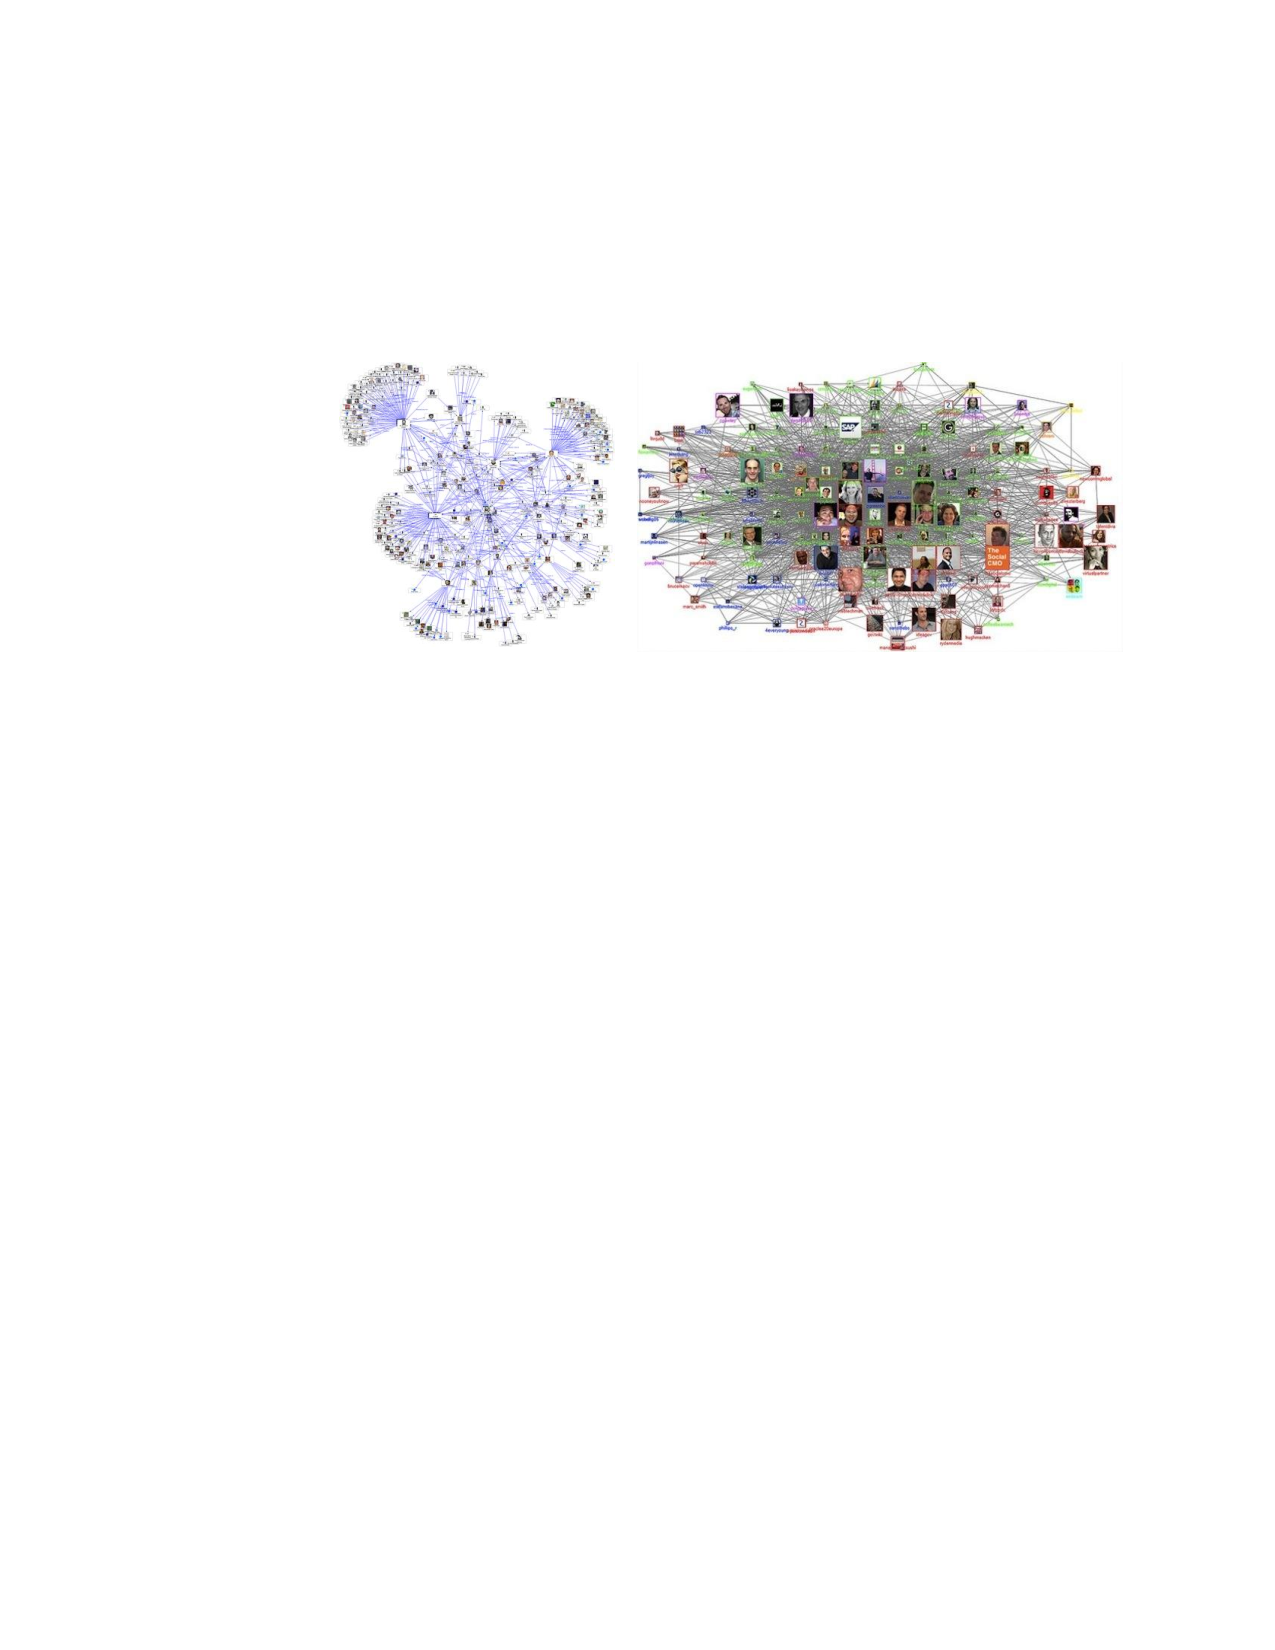
\includegraphics[width=0.7\textwidth]{Figure_1_3.pdf}
  \caption{Minh họa trực quan mạng xã hội}\label{fig:figure_1_3}
  (Nguồn: http://mashable.com/2012/09/26/graph-databases/\\
  http://www.fmsasg.com/SocialNetworkAnalysis/\\
  Truy cập lần cuối 20/01/2014)
\end{center}
\end{figure}

\subsubsection*{b) Biểu diễn mạng xã hội}
Một mạng xã hội (Social Network), ký hiệu SN, có thể được định nghĩa là một đồ thị gồm các thành phần cơ bản như sau:
\begin{equation}
SN = (V, E, L(V), L(E))
\end{equation}
Trong đó,
\begin{itemize}
\item V: tập các actor hay còn gọi là các nút trong mạng.
\item $E \subseteq V$x$V$: tập các cạnh của đồ thị hay các mối quan hệ trong mạng.
\item L(V): tập các nhãn nút.
\item L(E): tập các nhãn cạnh.
\end{itemize}

Tùy vào mỗi bài toán cụ thể, các nút, cạnh thuộc mạng có cấu trúc và ngữ nghĩa khác nhau. Tức với mỗi bài toán, chúng ta có thể dùng đơn đồ thị có hướng, vô hướng hoặc đa đồ thị để mô hình hóa các mạng xã hội tương ứng.

\subsubsection*{c) Phân tích Mạng xã hội}
Nghiên cứu về các mạng xã hội còn được gọi là phân tích mạng xã hội, viết tắt là SNA. Theo tác giả Serrat \cite{serrat2009social}, SNA tập trung vào phân tích cấu trúc của những quan hệ. SNA giả sử rằng các mối quan hệ là rất quan trọng và tìm cách tính toán, đo lường các mối quan hệ một cách hình thức và không hình thức để hiểu được những gì đã tạo điều kiện hay cản trở những luồng thông tin di chuyển, lan truyền trong mạng. SNA được sử dụng rộng rãi trong khoa học xã hội và khoa học hành vi, trong kinh tế, tiếp thị cũng như công nghệ và được xem như một kỹ thuật chính trong khoa học xã hội hiện đại \cite{Wasserman1994}. 

Ngành xã hội học đã nghiên cứu và đưa ra một số nguyên tắc có thể ứng dụng trong quá trình phân tích các mạng xã hội. Trong đó homophily, proximity là những nguyên tắc cơ bản và được quan tâm.
\begin{itemize}
\item \textbf{Nguyên tắc `homophily'}. Những nhà xã hội học đã đưa ra nguyên tắc: "Sự tương tự tạo ra những kết nối", đó chính là nguyên tắc `homophily' trong khoa học xã hội và hành vi. Nguyên tắc này đã hình thành nên những kết nối và cấu trúc xã hội với nhiều kiểu quan quan hệ khác nhau như: bạn bè, vợ chồng, đồng nghiệp, đồng thành viên và nhiều kiểu quan hệ khác. `Homophily' đã tạo ra những phân chia mạnh mẽ nhất trong môi trường cá nhân của chúng ta với tuổi tác, tôn giáo, nghề nghiệp, giới tính \cite{mcpherson2001birds}. \label{concept:homophily}
\item \textbf{Nguyên tắc `proximity'}. Trong lĩnh vực tâm lý xã hội, nguyên tắc `proximity' cho biết các cá nhân có xu hướng hình thành những mối quan hệ với những người ở gần. Tức những người gặp nhau thường xuyên, sống và làm việc gần nhau thì dễ hình thành và phát triển quan hệ.\label{concept:proximity}
%\item \textbf{Nguyên tắc `elaboration'.}
%\item \textbf{Nguyên tắc `Similarity'.}
%\item \textbf{Nguyên tắc `Complementarity'.}
%\item \textbf{Nguyên tắc `Reciprocity'.}
%\item \textbf{Nguyên tắc `Minimax'.}
%http://nber.org/papers/w11530
\end{itemize}

\subsubsection{Khuyến nghị xã hội (Social Recommendation)}
Hệ khuyến nghị truyền thống giả sử những người dùng trong hệ thống độc lập với nhau, chưa xem xét những tương tác cũng như quan hệ xã hội của họ. Trong khi, các mối quan hệ xã hội có vai trò rất quan trọng, ảnh hưởng đến sở thích, hành vi và quyết định của con người. Chẳng hạn, chúng ta thường xin ý kiến tư vấn, đề xuất của người thân, bạn bè, thầy cô, đồng nghiệp để thực hiện một quyết định như: mua một sản phẩm, xem một cuốn phim, tìm kiếm nhà hàng, chọn một công việc, đọc một cuốn sách, tìm một bài báo, chọn một đối tác. Thật ra, đó là quá trình yêu cầu các khuyến nghị dựa trên các mối quan hệ xã hội, gọi tắt là khuyến nghị xã hội.

Việc nghiên cứu phát triển các phương pháp khuyến nghị xã hội đã thu hút nhiều quan tâm nghiên cứu của cộng đồng từ khi các mạng xã hội ra đời và phát triển. Tiếp cận khuyến nghị xã hội bổ sung việc xem xét sở thích của người dùng dựa trên việc phân tích, khai thác các thông tin từ các mạng xã hội như: đánh giá của người dùng từ các trang mạng xã hội, mức độ ảnh hưởng của các mối quan hệ xã hội đến sở thích của người dùng. Với khuyến nghị xã hội, bên cạnh ma trận đánh giá của người dùng, thông tin đầu vào còn có ma trận thể hiện mối quan hệ giữa những người dùng (hình \ref{fig:figure_1_4}).

\begin{figure}[ht]
\begin{center}
  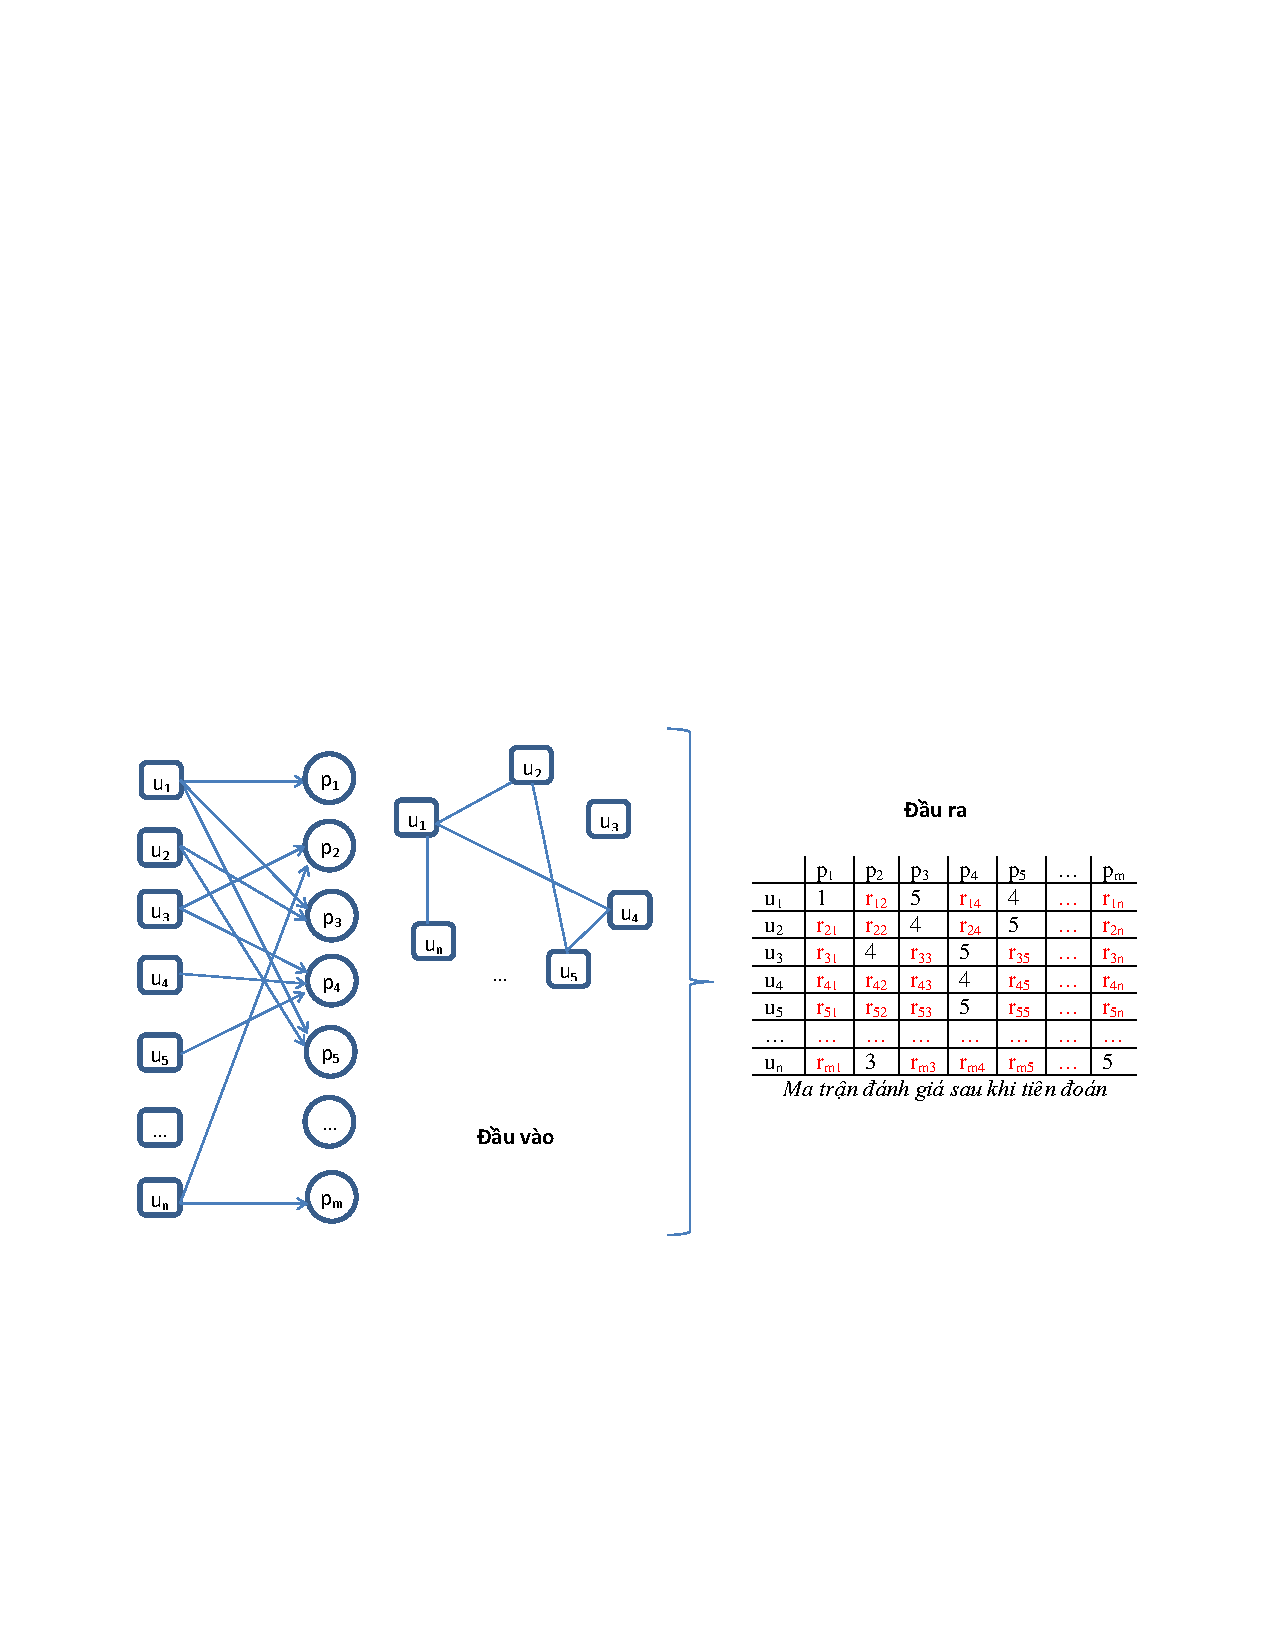
\includegraphics[width=0.75\textwidth]{Figure_1_4.pdf}
  \caption{Minh họa khuyến nghị xã hội}\label{fig:figure_1_4}
\end{center}
\end{figure}

Tác giả Tang và cộng sự đã khảo sát và hệ thống lại những tiếp cận khuyến nghị truyền thống, thảo luận một số hướng nghiên cứu mới cho hệ khuyến nghị và đã tập trung vào hướng phân tích mạng xã hội cho khuyến nghị hay khuyến nghị xã hội (Social Recommendation) \cite{JiliangTang:2013SocialRecommendation}. Tác giả cũng đã phát biểu một cách hình thức bài toán khuyến nghị xã hội và xác định khuyến nghị xã hội vẫn đang ở giai đoạn của những bước đi đầu tiên cần đầu tư nghiên cứu phát triển. Tác giả cũng đã chỉ ra một số hướng nghiên cứu tiềm năng nhằm cải tiến các khuyến nghị xã hội như: khai thác tính không đồng nhất của các mạng xã hội và những liên kết phụ thuộc yếu, khai thác các mối quan hệ tiềm ẩn, quan hệ lòng tin, xem xét thông tin thời gian của các đánh giá. 

Tác giả Aranda và cộng sự đã trình bày một hệ thống khuyến nghị dựa trên mạng xã hội. Hệ thống được hiện thực dùng dữ liệu thu thập từ trang web trò chơi BGG.\footnote{http://boardgamegeek.com/} Mục đích của hệ thống là giới thiệu các trò chơi mới cho các thành viên của BGG thông qua quá khứ đánh giá và các mối quan hệ của họ \cite{aranda2007online}.

Tác giả Ma và cộng sự đã dựa trên quan điểm "mạng xã hội của người dùng sẽ ảnh hưởng đến hành vi của họ trên web" để đề xuất phương pháp khuyến nghị xã hội mới. Phương pháp đề xuất hợp nhất ma trận đánh giá với mạng xã hội người dùng bằng cách thừa số hóa ma trận đánh giá. Kết quả thực nghiệm của họ đã cho thấy phương pháp khuyến nghị xã hội đề xuất cho kết quả tốt hơn những thuật toán CF phổ biến, và nó có thể mở rộng cho những tập dữ liệu lớn \cite{Ma:2008:SSR}. 

Tác giả Esslimani và cộng sự đã đề xuất một tiếp cận lọc cộng tác mới dựa trên mạng hành vi (Behavioral Network Collaborative Filtering - BNCF) dùng những mẫu định liên quan đến định hướng để mô hình quan hệ giữa những người dùng và áp dụng kỹ thuật lan truyền trong mạng xã hội để khai thác thêm những liên kết tiềm ẩn thông qua mạng hành vi. Mục đích của BNCF là kết hợp cả những liên kết mới, tiềm ẩn để thực hiện tiên đoán, cải tiến chất lượng khuyến nghị. Độ chính xác tiên đoán dùng BNCF được đánh giá thông qua các tập dữ liệu thực. Kết quả thực nghiệm của họ cho thấy lợi ích của việc khai thác các liên kết mới, tiềm ẩn để tính toán tiên đoán. Các tác giả đã cho thấy BNCF cải tiến độ chính xác tiên đoán dựa trên phân tích lỗi trung bình MAE (Mean Absolute Error) và HMAE (High MAE) \cite{Esslimani:2009:BehavioralNetwork}.

Tác giả Davoodi và cộng sự đã đề xuất một phương pháp lai, kết hợp những đặc điểm của các thuật toán dựa trên nội dung vào hệ thống lọc CF dựa trên mạng xã hội để khuyến nghị chuyên gia \cite{Davoodi:2012:SNA}. Phương pháp của họ nhằm cải tiến độ chính xác tiên đoán dựa trên việc xem xét khía cạnh xã hội, hành vi của chuyên gia. Phương pháp của họ bao gồm một số bước chính như: xác định những cộng đồng xã hội của những chuyên gia, chỉ định những thành viên đại diện trong mỗi cộng đồng dùng các độ đo trung tâm (centrality measure) (\citet{LarsKirchhoff:2008:SNAEnhanceIR}), và cuối cùng là khuyến nghị những chuyên gia đại diện cộng đồng liên quan nhiều nhất với người dùng đang có nhu cầu tìm kếm chuyên gia. Độ chính xác tiên đoán trong thực nghiệm của họ cho thấy, việc dùng thông tin mạng xã hội đã có cải thiện so với phương pháp không dùng thông tin mạng xã hội. Kết quả tiên đoán là 78.4\% so với 75.6\% với độ đo Precision cho Top-5 (P@5) \cite{Davoodi:2012:SNA}.

Các tác giả Abbasi và Altmann đã đề xuất hệ thống AcaSoNet dùng để xác định và quản lý mạng xã hội của những người nghiên cứu \cite{Abbasi:2009:SocialNet}. AcaSoNet được dùng để phân tích, đánh giá hoạt động của những người nghiên cứu. AcaSoNet đã rút trích và thu thập dữ liệu của những người nghiên cứu từ www, đồng thời cho phép người dùng cập nhật dữ liệu của họ. Mạng xã hội của những người nghiên cứu được xác định dựa trên kho dữ liệu bài báo thu thập. Hiện nay AcaSoNet chỉ cung cấp giao diện và dữ liệu phục vụ cho phân tích mạng xã hội. Sắp đến, họ dự định sẽ cung cấp thêm các dịch vụ khác như khuyến nghị bài báo, gom cụm cộng đồng nghiên cứu, v.v...

Tác giả Tang và cộng sự đã đề xuất hệ thống ArnetMiner nhằm rút trích và khai thác những mạng xã hội học thuật \cite{Tang:2008:ArnetMinner}. ArnetMiner bao gồm các môđun chính như: (1) Rút trích hồ sơ người nghiên cứu từ www; (2) Tích hợp dữ liệu bài báo từ các thư viện số hiện có; (3) Mô hình hóa các mạng xã hội học thuật, chủ yếu là mạng đồng tác giả và mạng trích dẫn; (4) Cung cấp các dịch vụ tìm kiếm trựa trên các mạng xã hội học thuật. Vào thời điểm công bố, ArnetMiner có 448.470 hồ sơ nghiên cứu viên, hệ thống cũng đã tích hợp hơn 1.000.000 bài báo khoa học.

Tác giả Brandao và cộng sự đã xem xét hai nguyên tắc xã hội là `homophily' (mục \ref{concept:homophily}) và `proximity' (mục \ref{concept:proximity}) để đề xuất hai độ đo mới cho khuyến nghị cộng tác trong mạng xã hội học thuật \cite{Brandao:2013:ULS}. Hai độ đo đề xuất lần lượt xem xét yếu tố cơ quan công tác và thông tin vị trí địa lý của nghiên cứu viên. Đồng thời nhóm tác giả cũng dựa trên những khái niệm xã hội như: tính mới, tính đa dạng, tính bao phủ, để đề xuất các độ đo mới nhằm đánh giá kết quả khuyến nghị. Kết quả thực nghiệm của họ cho thấy các phương pháp đề xuất cho kết quả tốt hơn những phương pháp phổ biến hiện nay.

Năm 2008, Ijad Madisch và cộng sự đã xây dựng và phát triển hệ thống mạng xã hội trong lĩnh vực học thuật, đặt tên là ResearchGate\footnote{https://www.researchgate.net/about}. ResearchGate là một trang mạng xã hội học thuật, giúp các nhà khoa học, nghiên cứu viên chia sẻ bài báo khoa học, kiến thức và kinh nghiệm nghiên cứu thông qua việc cập nhật danh sách bài báo công bố, thảo luận, hỏi đáp. Bên cạnh đó ResearchGate giúp các nghiên cứu viên tìm kiếm việc làm phù hợp với kinh nghiệm và năng lực nghiên cứu, hỗ trợ tìm kiếm chuyên gia để hợp tác nghiên cứu. ResearchGate thực hiện khá hiệu quả việc chia sẻ thông tin học thuật. Thông tin bài báo trên ResearchGate được chia sẻ, khuyến nghị cho người dùng thông qua các mối quan hệ tường minh (quan hệ follow) do người dùng chủ động cập nhật. ResearchGate chứa rất nhiều thông tin học thuật liên quan các nhà khoa học, nghiên cứu viên, bài báo, các trường, viện. Tuy nhiên, theo hiểu biết của nghiên cứu sinh thì dữ liệu của ResearchGate hiện không chia sẻ, cho phép tải về để thực hiện các nghiên cứu. Bên cạnh đó, chức năng khuyến nghị của ResearchGate còn khá đơn giản, chỉ xem xét mỗi quan hệ tường minh, chưa xem xét các quan hệ tiềm ẩn, trung gian, cũng như các quan hệ học thuật khác như quan hệ trích dẫn, quan hệ hợp tác giữa các cơ quan và những đặc trưng khác của nghiên cứu viên. 

Một vấn đề khá quan trọng khác cần xem xét khi đề cập đến các mối quan hệ xã hội đó là khái niệm lòng tin (trust). Lòng tin có thể xem là thuộc tính của quan hệ xã hội. Theo Touhid Bhuiyan, 2013 \cite{Bhuiyan:2013:TIR:2469991}, có nhiều định nghĩa khác nhau cho khái niệm lòng tin, nhưng định nghĩa được đa số cộng đồng trích dẫn và sử dụng là định nghĩa của nhà xã hội học Dasgupta. Lòng tin là sự mong đợi của một người về những hành động của người khác mà có ảnh hưởng đến quyết định, lựa chọn của họ \cite{Dasgupta1988-DASTAA}. Theo Piotr Sztompka, 1999 \cite{Sztompka1999}, lòng tin gồm hai thành phần chính là tin tưởng (belief) và cam kết (commitment). Tức một người sẽ tin tưởng rằng một người khác sẽ hành động theo một cách nhất định và đặt lòng tin vào họ, nhưng sự tin tưởng không thôi thì chưa đủ để có lòng tin. Lòng tin được đặt vào một ai đó khi sự tin tưởng đạt tới mức độ làm nền tảng cho một cam kết thực hiện một hành động cụ thể. Gần đây, lòng tin đã trở thành một chủ đề nghiên cứu quan trọng trong nhiều lĩnh vực như: xã hội học, tâm lý học, và cả tin học.

Stephen Marsh là một trong những người đi tiên phong trong việc khai thác lòng tin trong tính toán khoa học \cite{Marsh:1994}. Gần đây, lòng tin đã thu hút nhiều quan tâm nghiên cứu của cộng đồng trong việc phát triển các hệ thống khuyến nghị trực tuyến. Người dùng thường sẽ tin tưởng và dễ dàng chấp nhận các khuyến nghị từ bạn bè, người thân hơn là những người lạ khác, ngay cả khi hệ khuyến nghị có những đề xuất hữu ích và chất lượng. Bên cạnh đó, lòng tin được sử dụng để cải tiến các phương pháp khuyến nghị truyền thống. Việc sử dụng quan hệ lòng tin giúp các hệ khuyến nghị có thể đương đầu với những khó khăn, thách thức như: ma trận đánh giá thưa, khởi động lạnh (cold-start).

Paolo Massa và Paolo Avesani đã đề xuất thay thế bước tính toán tương tự người dùng trên ma trận đánh giá bằng độ đo lòng tin giữa những người. Họ đề xuất thuật toán lan truyền lòng tin trên mạng và tính mức độ lòng tin giữa những người dùng. Kết quả thực nghiệm trên tập dữ liệu Epinions cho thấy việc khai thác lòng tin cải tiến độ chính xác khuyến nghị \cite{Massa:2007:TRS:1297231.1297235}. Hao Ma và cộng sự đã nghiên cứu đề xuất phương pháp tối ưu dựa trên kết hợp cả các mối quan hệ lòng tin và không tin (distrust) nhằm cung cấp các khuyến nghị chính xác và thực tế cho người dùng. Nhóm tác giả cũng đã thực nghiệm trên tập dữ liệu Epinions và cho thấy hương pháp của họ tốt hơn hẳn các phương pháp hiện có trên tập dữ liệu này \cite{Ma:2009:LRT:1639714.1639746}. Lahiru S. Gallege và cộng sự đã nghiên cứu khai thác lòng tin để hướng đến phát triển hệ khuyến nghị cho các dịch phần mềm trực tuyến \cite{Gallege:2014:TTR:2602087.2602118}.

Trong lĩnh vực học thuật, theo hiểu biết của nghiên cứu sinh thì khái niệm lòng tin, những mối quan hệ tiềm ẩn, yếu tố xu hướng sở thích nghiên cứu, xu hướng quan hệ chưa được đề cập và khai thác để phát triển các phương pháp khuyến nghị thông tin cho nghiên cứu viên. 

Nhìn chung các phương pháp khuyến nghị xã hội có những thuận lợi và khó khăn như sau:

\begin{itemize}
	\item \textbf{Thuận lợi}: độc lập lĩnh vực, không phụ thuộc vào đối tượng khuyến nghị. Có thể đương đầu với vấn đề ma trận đánh giá thưa, người dùng mới. Kết hợp thông tin quan hệ xã hội với các thông tin khác có thể cải tiến độ chính xác tiên đoán, chất lượng khuyến nghị.
\end{itemize}
\begin{itemize}
	\item \textbf{Khó khăn, thách thức}: Việc xác định các mối quan hệ xã hội (rõ ràng và tiềm ẩn). Làm thế nào để lượng hóa được mức độ ảnh hưởng của các mối quan hệ xã hội đến sở thích, hành vi và quyết định của người dùng. Làm thế nào để kết hợp thông tin về các mối quan hệ xã hội với những thông tin khác để phát triển các phương pháp lai.
\end{itemize}

Đây là hướng tiếp cận chính của luận án nhằm phát triển các phương pháp khuyến nghị mới để hỗ trợ nghiên cứu viên đương đầu với tình trạng quá tải thông tin trong lĩnh vực học thuật. Luận án chọn tiếp cận phân tích mạng xã hội nhằm giải quyết những khó khăn, thách thức mà các phương pháp truyền thống đang đương đầu, đó là: vấn đề người dùng mới, đối tượng khuyến nghị mới (khởi động lạnh); ma trận đánh giá thưa, thiếu hoặc không có thông tin đánh giá của người dùng; vấn đề chất lượng tiên đoán, khuyến nghị. 

\section{Các phương pháp đánh giá hệ khuyến nghị}
\subsection{Phương pháp thiết lập thực nghiệm}
Các tác giả Gunawardana và Shani đã chỉ ra rằng, thông thường sẽ có hai cách thiết lập thực nghiệm để đánh giá hệ khuyến nghị. Đó là thiết lập đánh giá online và thiết lập đánh giá off-line, gọi tắt là đánh giá online và đánh giá off-line \cite{GunawardanaS09}. 
\begin{itemize}
\item \textbf{Đánh giá Online}: Mục đích của đánh giá online là đo lường sự thay đổi hành vi người dùng khi họ tương tác với hệ khuyến nghị. Hay nói cách khác, chúng ta cần xem xét hệ khuyến nghị đã ảnh hưởng như thế nào đến việc thay đổi hành vi người dùng, khi họ tương tác với nó. Ưu điểm của đánh giá online là phản ánh đúng hiệu năng thật sự của hệ khuyến nghị khi người dùng tương tác với nó. 

Với đánh giá online thì hệ khuyến nghị cần được triển khai sử dụng thật sự. Nhưng khó khăn là chúng ta cần thực nghiệm và kiểm tra một loạt nhiều thuật toán khuyến nghị xem cái nào là phù hợp trước khi đưa vào sử dụng. Đây giống như trường hợp "Quả trứng và con gà". Bên cạnh đó, việc đánh giá online cần phải xem xét vấn đề đánh giá ở nhiều góc độ khác nhau như: cố định giao diện, thay đổi thuật toán và ngược lại. Như vậy, để thực hiện đánh giá online sẽ tốn nhiều chi phí. Vì vậy hầu hết các nghiên cứu hiện nay đều sử dụng phương pháp đánh giá off-line.
\item \textbf{Đánh giá off-line}: Với đánh giá off-line, các nghiên cứu cần đưa ra giả thuyết "Giả sử kết quả thực nghiệm off-line là tương quan với hành vi người dùng online". Tức chúng ta mong đợi và giả sử rằng nếu như đánh giá off-line đạt hiệu quả tốt thì khi triển khai Online cũng vậy. 

Để thực hiện đánh giá off-line, cần thiết phải giả lập hay mô phỏng tốt quá trình online khi hệ thống thực hiện khuyến nghị và người dùng sử dụng các kết quả khuyến nghị. Thông thường, các nghiên cứu phải lưu lại dữ liệu lịch sử người dùng. Sau đó ẩn đi những tương tác của người dùng để xem người dùng sẽ quan tâm, hay hành động như thế nào với các đối tượng sẽ được khuyến nghị thông qua việc áp dụng những phương pháp khuyến khác nhau.
\end{itemize}

\subsection{Độ đo đánh giá}
Các độ đo đánh giá hệ khuyến nghị có nguồn gốc từ các phương pháp đánh giá trong lĩnh vực học máy và truy vấn thông tin. Cùng với việc chọn lựa cách thiết lập đánh giá, là online hay off-line, các tác giả Gunawardana và Shani đã phân loại hệ khuyến nghị thành 3 nhóm chính dựa trên công việc thực hiện khuyến nghị và chỉ ra những độ đo đánh giá phù hợp với mỗi nhóm \cite{GunawardanaS09}.

\subsubsection{Tiên đoán đánh giá}
Tiên đoán đánh giá tức hệ thống yêu cầu tiên đoán những đánh giá của người dùng dựa trên tập hợp các đối tượng khuyến nghị cho trước. Những ứng dụng phổ biến thường thấy với tiên đoán đánh giá là các website thương mại điện tử như Netflix\footnote{www.netflix.com}, CNET\footnote{www.cnet.com}. Chẳng hạn với Netflix, khi người dùng duyệt danh sách các phim mới thì hệ thống sẽ gán một giá trị tiên đoán đánh giá cho mỗi phim này. Những phim có giá trị tiên đoán đánh giá cao xem như ưu tiên khuyến nghị cho người dùng.

Độ đo thường dùng cho tiên đoán đánh giá là lỗi bình phương trung bình (Root of The Mean Square Error), viết tắt là RMSE (công thức \ref{equation:RMSE}) và các biến thể của nó như MAE (Mean Average Error), NMAE (Normalized Mean Average Error) \cite{Celma:2010:EvaluationMetrics, ShaniG11}. 

\begin{equation} \label{equation:RMSE}
RMSE = \sqrt{\frac{ \sum\limits_{(u,p) \in K}^{} (r_{u,p} - v_{u,p})^2}{n}}
\end{equation}

Trong đó,
\begin{itemize}
\item $r_{u,p}$: giá trị đánh giá của người dùng $u$ trên đối tượng $p$ hệ thống tiên đoán được.
\item $v_{u,p}$: giá trị đánh giá thật sự (đúng) của người dùng $u$ trên đối tượng $p$.
\item $K = \{(u,p)\}$: tập các đánh giá của người dùng $u$ trên đối tượng $p$ cần tiên đoán.
\item $n = |K|$: kích thước tập $K$.
\end{itemize}

RMSE được đánh giá là phù hợp cho công việc tiên đoán. Tuy nhiên nó thật sự phù hợp khi chúng ta không cần phân biệt giữa các lỗi đánh giá. Chẳng hạn, giá trị đánh giá thật sự của người dùng $u$ trên đối tượng $p$ là 2, nhưng kết quả hai phương pháp khác nhau cho ra lần lượt là 1 và 3. Khi đó tính độ lệch dùng RMSE cho kết quả như nhau. Nhưng thật ra ý nghĩa khuyến nghị sẽ khác nhau. Hay nói rõ hơn, phương pháp cho ra giá trị tiên đoán là 3 sẽ ưu tiên khuyến nghị đối tượng $p$ cho $u$, trong khi phương pháp cho ra giá trị đánh giá là 1 sẽ không mong muốn khuyến nghị $p$ cho $u$.

\subsubsection{Tối ưu tính hữu ích của hệ thống khuyến nghị}
Một nhóm các công việc khác của các hệ khuyến nghị là tối ưu tính hữu ích của hệ thống khuyến nghị. Như vậy đối với các công việc khuyến nghị dạng này là cần định nghĩa một hàm hữu ích, và xây dựng thuật toán để tối ưu hàm hữu ích này. Với mỗi bài toán khuyến nghị và mục tiêu khuyến nghị cụ thể, một hàm hữu ích sẽ được định nghĩa và tìm thuật toán để tối ưu hàm này. (\citet{GunawardanaS09}) đã phân ra hai dạng hàm hữu ích là hướng lợi nhuận và hướng người dùng.
\begin{itemize}
\item \textbf{Hướng lợi nhuận}: Nếu xét ở góc độ lợi nhuận của nhà cung cấp dịch vụ, chẳng hạn đối với một số trang web thương mại điện tử thì họ cần hệ thống khuyến nghị mà có thể cực đại hóa khả năng bán hàng, nhằm đạt được doanh số bán hàng cao nhất hoặc lợi nhuận nhiều nhất. Đối với các trang web tin tức quảng cáo thì hệ khuyến nghị cần khuyến nghị các mẫu tin dài, để giữ người dùng ở lại với trang web càng lâu càng tốt.

\item \textbf{Hướng người dùng}: Đôi khi người dùng quan tâm đến những đối tượng mới, chưa biết hơn những đối đối tượng quen thuộc, đã biết. Việc khuyến nghị các đối tượng quen thuộc đôi khi là dư thừa, không cần thiết. Vì vậy, hệ thống khuyến nghị hướng người dùng cần xem xét tính mới, tính đa dạng khi thực hiện khuyến nghị các đối tượng. Gần đây đã có một số các nghiên cứu bắt đầu xem xét tính mới, đa dạng khi thực hiện khuyến nghị. Các tác giả Zhang và Hurley đã nghiên cứu về tính mới, tính đa dạng trong khuyến nghị và đề xuất một phương pháp đánh giá cho phép phân tích hiệu năng của nhiều thuật toán khác nhau dưới góc độ khuyến nghị những đối tượng không những liên quan, nhưng phải mới \cite{ZhangH09, Hurley:2011:NDT}. Bên cạnh đó, Vargas và Castells cũng xác định những khái niệm nền tảng cho tính mới, đa dạng trong khuyến nghị và đề xuất một framework hỗ trợ phát triển các độ đo để đánh giá tính mới, đa dạng cho các thuật toán khuyến nghị \cite{Vargas:2011:RRN}.
\end{itemize} 

\subsubsection{Khuyến nghị các đối tượng tốt}
Công việc chung nhất của hầu hết các hệ khuyến nghị là đề xuất một danh sách các đối tượng được cho là phù hợp với sở thích người dùng. Kiểu khuyến nghị này thường thấy ở các trang web thương mại điện tử như: Amazon, Netflix. Khi người dùng chọn một sản phẩm nào đó, thì hệ thống sẽ khuyến nghị một danh sách các đối tượng khác được cho là liên quan đến nhu cầu, sở thích của người dùng. Theo tác giả Gunawardana và Shani \cite{GunawardanaS09}, các công việc khuyến nghị các đối tượng tốt có thể phân thành hai loại: (1) Một là khuyến nghị một vài đối tượng tốt (recommending some good items). Đây là các bài toán như khuyến nghị sách, phim, tin tức. Những bài toán đó, có một số lượng vô cùng lớn các phim, sách, tin tức liên quan đến người dùng cần khuyến nghị. Và hệ thống khuyến nghị chỉ nên khuyến nghị một vài đối tượng liên quan. Tránh khuyến nghị những đối tượng không liên quan sở thích hơn là phải khuyến nghị tất cả các đối tượng liên quan sở thích của người dùng; (2) Hai là tất cả các đối tượng khuyến nghị phải và nên tốt (recommending all good items). Chẳng hạn, bài toán khuyến nghị bài báo trích dẫn. Hệ thống cần tìm tất cả các bài báo tốt liên quan cần trích dẫn để khuyến nghị cho người dùng, tránh khuyến nghị các bài báo không liên quan đến công việc trích dẫn.

Để đánh giá danh sách các đối tượng khuyến nghị mà hệ thống đề xuất cho người dùng có phù hợp hay không, các nghiên cứu hiện nay thường sử dụng các độ đo có nguồn gốc truy vấn thông tin như: độ chính xác Precision (P), độ bao phủ Recall (R), và những độ đo có xem xét thứ tự xếp hạng của các đối tượng khuyến nghị trong danh sách đề xuất, đó là Mean Average Precision (MAP) \cite{Yue:2007:SVM:MAP}, NCDG \cite{Jarvelin:2000:IEM:NDCG}.

\section{Khó khăn, thách thức và xu hướng}
\subsection{Khó khăn, thách thức}
Một số khó khăn, thách thức chính đối với các phương pháp khuyến nghị truyền thống, phổ biến hiện nay có thể kể đến như sau:
\begin{itemize}
\item Dữ liệu lớn. Không gian người dùng và đối tượng khuyến nghị là rất lớn.
\item Độ chính xác, chất lượng khuyến nghị.
\item Vấn đề ma trận đánh giá thưa, tức số đánh giá quan sát được rất ít so với số đánh giá cần tiên đoán để khuyến nghị. Điều đó ảnh hưởng đến độ chính xác tiên đoán, chất lượng khuyến nghị.
\item Vấn đề khởi động lạnh (cold start). Quan sát thiếu hay không quan sát được một số thông tin về sở thích, đánh giá của người dùng, cũng như các đối tượng khuyến nghị. Hoặc làm thế nào để thực hiện khuyến nghị cho những người dùng mới hay đối tượng khuyến nghị mới.
\item Các phương pháp đánh giá kết quả khuyến nghị.

\end{itemize}
\subsection{Xu hướng mới cho hệ khuyến nghị}
Trong các nghiên cứu khảo sát về hệ khuyến nghị của Adomavicius và Tuzhilin \cite{Adomavicius:2005:TNG:1070611.1070751}, cũng như của Bobadilla và cộng sự \cite{Bobadilla2013109}, các tác giả đã chỉ ra những xu hướng mà cộng đồng đang quan tâm để phát triển các phương pháp khuyến nghị mới nhằm giải quyết những khó khăn, thách thức của các phương pháp truyền thống. Một số xu hướng khuyến nghị mới có thể kể đến như sau:
\begin{itemize}
\item Stefanidis và cộng sự cũng chỉ ra rằng, các phương pháp truyền thống chưa quan tâm xem xét sự ảnh hưởng của yếu tố thời gian, xu hướng đến kết quả khuyến nghị như thế nào \cite{StefanidisNNK12}.
\item Làm thế nào để kết hợp thông tin xã hội rõ ràng, cũng như tiềm ẩn vào các phương pháp truyền thống. 
\item Sử dụng thông tin nhận biết ngữ cảnh (context-aware) để thực hiện khuyến nghị. Liên quan đến tiếp cận khai thác thông tin ngữ cảnh, Gediminas Adomavicius và cộng sự khảo sát phân tích các nghiên cứu khác nhau \cite{AdomaviciusMRT11, AdomaviciusT11}. Thông tin ngữ cảnh giúp các hệ khuyến nghị cung cấp những khuyến nghị phù hợp với người dùng theo thời gian, địa điểm. Cùng với sự phát triển mạnh mẽ của công nghệ di động, hướng tiếp cận khai thác thông tin ngữ cảnh được đánh giá là rất tiềm năng đối với các hệ khuyến nghị trên thiết bị di động.
\item Tiếp cận lai nhằm giải quyết những hạn chế của mỗi phương pháp khác nhau \cite{Robin:2002:HybridRS_Survey, Adomavicius:2005:TNG:1070611.1070751, Bobadilla2013109}.
\item Thu thập, sử dụng thông tin tiềm ẩn của người dùng từ Internet để xác định sở thích của họ.
\item Trong các nghiên cứu \cite{GunawardanaS09, ShaniG11, ShaniG13}, nhóm tác giả Gunawardana và Shani đã chỉ ra rằng, với mỗi bài toán cần có phương pháp khuyến nghị phù hợp. Đồng thời với mỗi phương pháp khuyến nghị, cũng cần có phương pháp đánh giá phù hợp. Tức phương pháp đánh giá sẽ quyết định độ chính xác tiên đoán, kết quả của phương pháp khuyến nghị. Việc nghiên cứu phát triển các phương pháp đánh giá kết quả khuyến nghị cũng nằm trong xu hướng và quan tâm của cộng đồng.
\end{itemize}

Tóm lại, những ưu điểm, hạn chế của các cách tiếp cận phổ biến hiện nay và xu hướng có thể trình bày tóm tắt trong bảng \ref{tab:table_1_2} ở cuối chương.
\begin{table}[ht]
\centering
    \caption{Tóm tắt ưu nhược điểm những tiếp cận phổ biến và xu hướng nghiên cứu}\label{tab:table_1_2}
    \begin{tabular}{|p{5.5cm}|p{1.5cm}|p{1.5cm}|p{1.5cm}|p{1.5cm}|p{1.5cm}|}
    \hline
    \multicolumn{1}{|c|}{\multirow{3}{*}{Ưu điểm \& Hạn chế}} & \multicolumn{5}{|c|}{Tiếp cận truyền thống và xu hướng} \\ 
    \cline{2-6}
    & \multicolumn{3}{|c|}{Truyền thống} & \multicolumn{2}{c|}{Xu hướng} \\
    \cline{2-6}
    & Nội dung (CB) & Lọc cộng tác (CF) & CB kết hợp CF & Phân tích mạng xã hội & Khai thác thông tin ngữ cảnh\\
    \hline
	Phù hợp đối tượng dạng văn bản & Có & Có & Có & Có & Có \\ 
	\hline
	Đa dạng đối tượng khuyến nghị & Không & Có & Có & Có & Có \\
	& & & & & \\
	\hline
	Hạn chế về phân tích nội dung & Có & Không & Không & Không & Không \\
	& & & & & \\
	\hline
	Có thể đa dạng hóa khuyến nghị. (Ngoài lĩnh vực quan sát) & Không & Có & Có & Có & Có \\
	\hline
	Người dùng mới. (Vấn đề khởi động lạnh) & Có & Có & Có & Có & Có \\
	\hline
	Đối tượng khuyến nghị mới. (Vấn đề khởi động lạnh) & Không & Có & Có & Có & Có \\
	\hline
	Vấn đề ma trận đánh giá thưa. & Không & Có & Có & Có & Có \\
	& & & & & \\
	\hline
	Có khả năng giải quyết vấn đề ma trận thưa và khởi động lạnh & Không & Không & Có & Có & Có \\
	\hline
	\end{tabular} 
	\begin{tabular}{|p{15.2 cm}|}
	\hline
	\textbf{Khó khăn chung:} \\
	(*) Dữ liệu lớn. \\
	(*) Độ chính xác, chất lượng khuyến nghị chưa cao. \\
	(*) Dữ liệu đánh giá thưa. \\
	(*) Chưa có phương pháp tốt để đánh giá kết quả, chất lượng khuyến nghị. \\
	(*) Vấn đề khởi động lạnh. \\
	\hline
	\end{tabular}
\end{table}

\section{Kết chương}
Chương này đã trình bày tổng quan về bài toán khuyến nghị trong trường hợp tổng quát và tập trung phân tích ưu điểm, hạn chế của các phương pháp khuyến nghị truyền thống. Bên cạnh những tiếp cận truyền thống cho hệ khuyến nghị, chương này cũng trình bày về xu hướng nghiên cứu, cũng như những tiếp cận mới cho hệ khuyến nghị mà cộng đồng đang quan tâm nghiên cứu, đó chính là các phương pháp tiếp cận lai, kết hợp phân tích mạng xã hội, xu hướng sử dụng thông tin nhận biết ngữ cảnh, cũng như khai thác thông tin tiềm ẩn của cá nhân từ "Internet of Things". Trên cơ sở khảo sát các nghiên cứu liên quan, mục tiêu và phạm vi luận án là tập trung pháp triển các phương pháp khuyến nghị lai dựa trên tiếp cận khai thác quan hệ xã hội, một tiếp cận có thể cải tiến độ chính xác tiên đoán, chất lượng khuyến nghị, có thể giải quyết được vấn đề dữ liệu đánh giá thưa, trường hợp người dùng mới (chưa có thông tin lịch sử về sở thích của người dùng).

Trong lĩnh vực học thuật, những kết quả thống kê (hình \ref{fig:figure_0_1}) cho thấy thông tin bài báo khoa học bùng nổ rất nhanh chóng, gây rất nhiều khó khăn cho những người làm nghiên cứu trong việc tìm kiếm tài liệu, chuyên gia, để thực hiện các công việc nghiên cứu. Vì vậy luận án hướng đến phát triển các phương pháp khuyến nghị nhằm hỗ trợ cộng đồng học thuật. Những bài toán đặt ra trong phạm vi của luận án thuộc nhóm phát triển các phương pháp khuyến nghị các đối tượng tốt cho người dùng. Tức là, để đánh giá kết quả khuyến nghị luận án đã sử dụng các độ đo như: độ chính xác Precision (P), độ chính xác top N (P@N), Recall (R), Mean Everage Precision (MAP).

Với dữ liệu, thông tin thu thập được, luận án chọn tiếp cận khai thác các mối quan hệ xã hội kết hợp yếu tố thời gian, không gian cho khuyến nghị. Để thực hiện được việc khai thác các mối quan hệ xã hội trong học thuật, chương tiếp theo sẽ trình bày việc rút trích, mô hình hóa các mạng xã hội trong lĩnh vực học thuật từ kho dữ liệu bài báo khoa học.
